\documentclass[UTF8,a4paper,12pt]{ctexart}

\newcommand{\ReportTitle}{面向城市复杂场景的生物启发式感知技术及产业应用}
\newcommand{\ReportType}{技术报告}
\newcommand{\ReportDate}{2026年9月}
\newcommand{\ReportHeaderLeft}{清华大学深圳国际研究生院}
\newcommand{\ReportHeaderRight}{2026年鉴定材料-技术报告}
\newcommand{\ReportUnits}{%
  清华大学深圳国际研究生院\\
  清华大学\\
  浙江大学\\
  深圳市智慧城市科技发展集团有限公司\\
  深圳天珑移动技术股份有限公司\\
  深圳创维显示科技有限公司\\
  深城交科技集团股份有限公司%
}

\usepackage{technicalreportstyle}
\setcounter{tocdepth}{2}

\begin{document}

\pagenumbering{roman}
\makeTechnicalReportCover

\begingroup
  \setcounter{tocdepth}{2}
  \setstretch{1.30}
  \renewcommand{\contentsname}{目录}
  \titleformat{name=\section,numberless}[block]
    {\centering\heiti\zihao{3}}
    {}
    {0pt}
    {}
  \titlespacing*{\section}{0pt}{0pt}{18pt}
  \pagestyle{tocpage}
  \makeatletter
  \let\ps@plain\ps@tocpage
  \makeatother
  \tableofcontents
  \clearpage
\endgroup

\pagenumbering{arabic}
\setcounter{page}{1}
\pagestyle{reportpage}

\section{引言}

\subsection{国家战略与发展需求}

建设数字中国是数字时代推进中国式现代化的重要引擎，也是构筑国家竞争新优势的重要支撑。《数字中国建设整体布局规划》明确提出，要夯实数字基础设施和数据资源体系，强化数字技术创新能力，全面提升数字中国建设的整体性、系统性和协同性\footnote{政策来源：中共中央、国务院，《数字中国建设整体布局规划》，2023年2月；\href{https://www.gov.cn/zhengce/2023-02/27/content_5743484.htm}{中国政府网原文}。}。《关于深化智慧城市发展 推进城市全域数字化转型的指导意见》进一步将城市作为推进数字中国建设的综合载体，要求整合状态感知、建模分析、城市运行和应急指挥等能力，实现城市态势全面感知、趋势智能研判、协同高效处置和调度敏捷响应\footnote{政策来源：国家发展改革委、国家数据局、财政部、自然资源部，《关于深化智慧城市发展 推进城市全域数字化转型的指导意见》（发改数据〔2024〕660号），2024年5月；\href{https://www.ndrc.gov.cn/xxgk/zcfb/tz/202405/t20240520_1386326_ext.html}{国家发展改革委原文}。}。国务院《关于深入实施“人工智能+”行动的意见》则面向科技、产业、民生和治理等重点领域，提出推动人工智能与经济社会各行业各领域广泛深度融合，发展新一代智能终端和智能体，提升公共安全、防灾减灾、交通治理和生产运行等场景的智能化水平\footnote{政策来源：国务院，《关于深入实施“人工智能+”行动的意见》（国发〔2025〕11号），2025年8月；\href{https://www.cac.gov.cn/2025-08/27/c_1758018277755538.htm}{中央网信办转载的中国政府网原文}。}。上述国家战略部署表明，城市数字化转型正在从基础设施联网和数据汇聚，进一步迈向全域感知、智能理解与协同决策的新阶段。

与此同时，新型城市基础设施建设、韧性城市建设和新型工业化对感知技术提出了更具体的任务要求。国家层面的城市数字化转型部署已明确提出，推进城市公共设施数字化改造和智能化运营，统筹部署泛在、韧性的城市智能感知终端，并推动城市智能基础设施与智能网联汽车协同发展。城市道路、建筑、市政设施、工业园区和公共空间由此加快部署物联网终端、智能摄像头、雷达、无人机、移动机器人及车路协同设施，城市运行逐步由周期性人工巡查转向连续在线监测，由事后处置转向风险预测与主动干预。低空飞行、智能网联汽车、智能制造等新产业与新场景进一步拓展了感知对象的速度范围、尺度范围和空间范围：系统既要识别快速运动的车辆和飞行器，也要发现远距离细线、微小缺陷和弱小目标；既要在白天和常规天气下稳定运行，也要在暗光、雨雪、遮挡和强动态干扰下持续工作；既要支撑单一设备的实时控制，也要服务跨区域、多节点、多主体的协同行动\footnote{政策依据：发改数据〔2024〕660号第（八）项。}。

这些部署共同指向一个基础性问题：数字城市首先必须能够真实、连续、完整地感知物理城市。如果前端观测在极端条件下失真，后续算法就无法恢复已经丢失的关键状态；如果多源信息不能在有限通信资源下有效流动，再多的感知节点也难以形成全局认知；如果复杂任务只能依赖高成本模型进行集中式端到端计算，系统也难以满足城市运行所要求的低时延和高可靠性。因此，感知技术已不再只是摄像头或传感器的数据采集问题，而是贯穿物理信号获取、跨源信息组织、任务语义理解和行动决策的系统性问题。提升这一链条的极限感知能力、全域协同能力和复杂认知能力，是数字中国、智慧城市与“人工智能+”战略由基础设施建设走向实际治理效能的重要技术基础。

从数字化转型的演进过程看，城市智能化大体经历“设施数字化、数据资源化、业务智能化、决策协同化”的能力递进。设施数字化解决物理对象能否接入网络的问题，数据资源化解决不同部门、不同主体的数据能否汇聚和流通的问题，业务智能化解决数据能否支撑识别、预测与处置的问题，决策协同化则要求多个平台、多个智能体围绕共同目标形成实时联动。感知处于这条链路的起点，也决定着后续环节的能力上限：只有前端信息真实、及时且具有足够覆盖度，数据才能被有效组织，模型推理才能建立在可靠事实上，最终决策才具有可解释、可执行和可追溯的基础。

这一基础作用在典型城市应用中表现得尤为突出。在智慧交通与低空运行场景中，感知结果直接关联目标跟踪、航迹预测、冲突检测和运动控制，系统不仅要“识别到”，还要以足够高的更新频率持续输出状态；在智能制造与基础设施运维场景中，微小裂纹、细线结构和早期故障征兆往往尺度小、对比度低，需要在复杂背景下保留弱而关键的异常信息；在智能安防与应急处置场景中，暗光、烟雾、雨雪、遮挡和通信波动可能同时出现，系统还必须整合固定摄像头、移动终端、无人机与机器人等多方观测，形成对事件演化过程的整体判断。不同场景虽然任务对象各异，但共同要求感知体系由“单设备获得局部图像”升级为“多节点持续获得可信状态，并服务后续认知与行动”。

\subsection{城市复杂场景的感知需求与关键挑战}

智能感知是连接物理城市与数字城市的基础环节，也是支撑智慧交通、智能制造、智能安防和智慧应急等产业应用的共性关键技术。只有持续、准确地获取城市运行状态，并将分散、多源、异构的观测转化为可理解、可推理、可行动的信息，城市智能系统才能形成可靠的分析、决策和控制闭环。随着城市应用不断向高速动态、极端环境、广域覆盖和复杂任务延伸，感知技术所面对的需求呈现出三个显著趋势：一是需求极端化，感知对象由常规目标扩展至高速、微小和暗光目标；二是规模扩大化，感知范围由单点、单域扩展至空天地海多域以及海量节点协同；三是任务复杂化，系统能力由目标检测和几何测量扩展至复杂语义理解、空间认知与系统规划。传统感知体系在这些新需求下逐渐暴露出“看不清、看不全、看不透”的瓶颈。

上述需求变化并不是对传统感知指标的简单提高，而是带来了传感机理、信息组织方式和计算范式的共同变化。从项目所面向的典型应用看，关键挑战可以归纳为以下三个相互关联的层次。

\subsubsection{极端条件下单点感知能力不足}

在城市交通和低空飞行中，目标运动速度快、状态变化频繁，传统RGB帧相机受固定曝光和有限帧率制约，容易产生运动模糊并遗漏帧间变化，感知输出频率往往难以匹配飞行控制、避障和应急响应所需的高频状态反馈。在工业质检、基础设施巡检和安防监控中，待检测对象可能只占据少量像素，甚至小于单个像素的等效尺度；其边缘弱、纹理少，并容易与复杂背景混叠，传统基于外观纹理的识别方法难以稳定提取判别特征。在夜间安防、地下空间、雨雪天气和强明暗交替场景中，传统相机的动态范围和信噪比进一步下降，有效目标信号可能被背景噪声和环境干扰淹没。

这类问题表面上分别表现为高速目标难跟踪、微小目标难识别和暗光目标难感知，本质上则来自传统帧式成像对时间、空间和光照信息的统一采样方式。提高帧率通常会缩短曝光时间并降低单帧信噪比，提高空间分辨率又会增加数据量和计算负担，延长曝光则会加剧高速运动模糊，单纯通过堆叠像素、提高帧率或增大模型规模难以从根本上消除这些制约。因此，需要从感知机理出发，引入对亮度变化和运动信息进行异步响应的新型视觉传感方式，并针对事件信号的稀疏、异步和高时间分辨特性重新设计检测、定位与增强算法。

\subsubsection{大规模场景下全域协同观测不完备}

城市感知正在由单个摄像头、单台车辆和单架无人机，扩展到由固定设施、移动终端、边缘节点和云端平台共同组成的分布式网络。单个节点受视场、遮挡、量程和部署位置限制，只能获得局部观测；视觉、事件、雷达、惯性和点云等不同模态虽然能够提供互补信息，却具有不同的采样频率、空间坐标、数据密度与噪声规律。若缺少统一的时空表征与匹配机制，多种传感器的简单叠加不仅不能形成互补，反而可能因时间错位、空间偏差和特征冲突降低融合精度。

当节点数量和数据规模进一步增加时，信息交换本身也成为系统瓶颈。原始图像、点云和神经网络中间特征具有较高数据维度，在带宽有限、链路动态和端侧算力受限的条件下持续传输，会引发通信拥塞、处理延迟和能源消耗。与此同时，不同观测的价值和可靠性并不相同：部分节点掌握关键视角和关键时刻的信息，部分数据则高度重复；部分传感器在当前环境中可靠，另一些传感器可能因遮挡、漂移或恶劣天气产生失真。如果系统不能回答“不同信息如何互补、哪些信息值得传输、哪些观测应当采信”，就难以将多源数据真正转化为完备、实时、可信的全域观测。

\subsubsection{复杂任务中认知准确性与实时性难以兼顾}

感知系统的任务正在由目标类别、位置和轨迹等几何层信息，向事件关系、场景因果、空间语义、任务分解和协同规划等高层认知延伸。例如，城市应急系统不仅要发现烟雾、车辆和人群，还要区分正常生产与异常火情，结合道路拥堵状态规划救援路径；多无人机和无人车协同搜索不仅要识别目标，还要理解自然语言任务、维护全局空间记忆，并根据平台能力和实时观测持续调整分工。这些任务包含多步推理和长时程决策，依靠单一轻量模型往往难以获得足够的语义理解与泛化能力。

基础大模型和视觉语言模型为复杂认知提供了新的能力，但其高质量推理通常伴随较高的词元、显存、算力和时间开销。现实任务中，大量工作只是高频、局部、规则明确的感知与执行操作，并不需要每次调用大模型；若将简单任务、复杂任务、全局规划和局部控制全部集中到大模型中处理，会造成计算资源错配，并使推理延迟阻塞实时执行。另一方面，完全依靠小模型又难以处理开放语义、长链条任务和陌生环境。因此，需要明确大小模型、全局与局部规划模块以及不同智能体之间的能力边界，依据任务难度、空间尺度和信息价值进行动态认知卸载，使高阶模型集中处理真正需要复杂推理的问题。

\subsection{传统技术路线的局限与本项目的研究切入点}

面向上述需求，现有研究通常沿着提高传感器规格、扩大模型规模或增加感知节点数量三条路线提升系统性能，这些路线在常规场景中具有明确作用，但难以单独应对城市复杂环境中的多重约束。首先，提高图像分辨率和采样帧率会同步增加数据吞吐、存储和计算负担，而且固定曝光成像仍然受到运动模糊、光照变化和帧间信息缺失的制约。换言之，单纯增加数据量并不必然增加有效信息量；当真正决定任务的高速变化、弱小边缘或瞬态信号在采集阶段已经丢失时，后端模型规模的增长无法完整补回物理观测中不存在的信息。

其次，增加传感器和节点数量能够扩展覆盖范围，却也把问题由“信息不足”转化为“信息过量且质量不一”。全量上传原始数据、在云端进行集中融合的方式依赖稳定而充足的通信条件，难以适应移动平台、突发事件和大规模并发接入；对所有节点采用固定权重或静态融合规则，又无法反映遮挡、漂移、恶劣天气和任务变化造成的可靠性波动。全域感知因而不能仅以节点数量衡量，还应同时考察异构信息是否对齐、通信资源是否用在关键观测上，以及融合结果能否识别和抑制不可信信息。

再次，将复杂感知、语义理解和任务规划统一交给大型模型，虽然能够减少人工设计的中间环节，却可能把高频简单操作也纳入高成本推理过程。城市智能系统通常同时包含毫秒至秒级的状态更新、分钟级的任务调整以及更长时间尺度的全局规划，不同环节对于语义能力、计算精度和响应速度的要求并不相同。若缺少分层机制，高层推理可能阻塞底层控制，底层大量重复信息也会挤占高层模型的上下文与算力；若完全拆分，各模块之间又可能因缺少共享语义和任务反馈而形成新的信息孤岛。

基于此，本项目不把感知、通信、融合和推理视为相互独立的算法模块，而是以有效信息在系统中的产生、流动与利用为主线，从三个层面形成研究切入点：在信息产生阶段，利用动态视觉的变化触发机制提高极端场景中关键物理信号的获取效率；在信息流动阶段，利用多感官互补、选择传导和先验调节机制建立多源协同观测；在信息利用阶段，利用认知卸载机制把任务合理分配至大小模型、不同空间层级和异构智能体。三者共同解决“有限传感资源如何获得更关键的信息、有限通信资源如何传递更有价值的信息、有限计算资源如何完成更复杂的任务”这一贯穿全链路的核心矛盾。

\subsection{生物启发式感知的研究依据}

生物感知系统为突破上述瓶颈提供了重要启发。生物视觉通过不同感光与神经通路分工，实现对细节、运动和弱光信息的高效编码；生物多感官系统通过感官互补、选择传导和经验调节，在有限神经资源下形成完整而可信的环境认知；生物认知系统则通过快慢通路、记忆分层以及大脑与感觉运动系统之间的协作，将高频简单任务与低频复杂任务分开处理。借鉴这些机理，可以从传感、融合到推理重新组织机器感知过程，使有限的感知、通信和计算资源聚焦于最具任务价值的信息，从而拓展城市智能系统的感知极限与认知边界。

在视觉感知层面，生物视觉由不同类型的感光细胞和神经通路分别处理颜色、细节、亮度与运动变化。事件相机借鉴生物视网膜对变化刺激的响应方式：每个像素独立响应亮度变化，只在变化超过阈值时输出事件，从而避免重复记录静态背景，并以微秒级时间分辨率保留高速运动过程。由此，机器视觉可以由“按固定帧率完整记录场景”转向“按变化选择性记录信息”，为突破高速、微小和暗光场景中的成像限制提供新的传感基础\footnote{科学依据：G. Gallego等，``Event-based Vision: A Survey,'' IEEE TPAMI, 44(1):154--180, 2022，DOI: \href{https://doi.org/10.1109/TPAMI.2020.3008413}{10.1109/TPAMI.2020.3008413}。}。

在多源融合层面，生物体不会依赖单一感官形成对环境的全部判断。视觉能够描述空间结构和外观，听觉能够在视线受阻时提供方向和时序线索，触觉与本体感觉则能够反馈接触状态和自身运动。更重要的是，神经系统会根据任务、刺激强度和既有经验动态分配注意力：高价值刺激被优先传导，相互重复或无关的信息受到抑制，不同感官的可信程度也会随环境条件调整。这一机制提示，多传感器、多节点系统的关键并非无差别汇聚数据，而是首先形成跨模态互补，进而根据任务价值选择信息，最后结合先验知识判断信息是否可信。感官互补、选择传导与先验调节共同构成了全域协同融合的仿生依据。

在认知推理层面，人类可以通过外部动作、环境表征和工具改变任务的信息处理需求，降低内部认知负担，这一现象通常被概括为认知卸载。对应到机器系统，本项目将这一原则进一步抽象为模型与智能体之间的任务分工：将高频简单任务分配给轻量模型和局部智能体，将低频复杂任务交由基础大模型和全局规划模块，并利用分层记忆、空间分解和视觉词元筛选进一步减少冗余推理，使有限算力与任务复杂度相匹配\footnote{概念来源：E. F. Risko与S. J. Gilbert，``Cognitive Offloading,'' Trends in Cognitive Sciences, 20(9):676--688, 2016，DOI: \href{https://doi.org/10.1016/j.tics.2016.07.002}{10.1016/j.tics.2016.07.002}。}。

本项目所强调的“生物启发”并非对生物器官结构的机械复刻，而是提炼其中具有普适意义的信息处理原则：以变化触发代替均匀采样，以功能互补代替单源增强，以价值选择代替全量传输，以先验调节代替静态加权，以分层卸载代替集中计算。上述原则分别作用于感知信息的产生、传输、融合和理解过程，能够将三个看似不同的技术问题组织在统一的方法论之下。

\subsection{研究对象与总体思路}

本项目面向城市复杂场景，研究从物理信息获取、多源信息协同到复杂任务理解的生物启发式感知理论、方法与系统。研究对象不是单一传感器或单一识别算法，而是贯穿“感知接入---协同融合---认知推理”的完整信息处理链条：前端关注高速、微小和暗光目标能否被及时、清晰地观测；中端关注跨模态、跨时空和跨节点信息能否高效、可信地组织与融合；后端关注复杂语义、空间关系和系统任务能否在有限算力下准确、实时地理解与规划。

围绕上述研究对象，本项目以“让机器看得更清、看得更广、看得更透”为总体目标，以生物动态视觉、多感官协同和认知卸载机理为共同方法论，形成“单点感知能力增强---多点协同感知体系增强---复杂任务理解能力增强”的总体技术路线。其中，“看得更清”旨在突破传统成像在时间分辨率、空间分辨率和动态范围上的限制；“看得更广”旨在突破单一模态、单一节点和静态采信机制对全域观测的限制；“看得更透”旨在突破复杂任务对大模型、海量词元和集中式计算的过度依赖。三类研究相互衔接，分别回答“信息如何被有效获取”“信息如何被高效而可信地协同”“信息如何被准确而实时地理解”三个核心问题。

从基础研究角度看，本项目重点研究三类共性问题。第一，研究非均匀、异步脉冲信息在高速动态和低信噪比条件下的有效表征规律，探索时间分辨率、空间细节和环境鲁棒性之间新的协调方式；第二，研究异构模态和分布式节点之间的信息对应关系、任务价值度量与可信度演化规律，使多源观测能够在通信和计算约束下形成稳定一致的场景表达；第三，研究复杂任务在模型能力、空间层级和执行主体之间的合理分解机制，使语义理解、记忆规划和实时控制能够以不同时间尺度协同运行。这三类问题从信号表征、信息融合延伸到认知计算，构成本项目的主要研究边界。

从系统研究角度看，本项目强调算法、传感器、通信网络、边缘计算与智能体执行平台之间的协同设计。前端传感算法需要保留事件信号的高频与稀疏优势，中端融合算法需要适应真实网络中的带宽波动和节点异质性，后端推理算法需要考虑端侧设备的算力、时延和任务安全要求；各层输出既是下一层的输入，也会受到最终任务反馈的调节。通过这种端到端但非单体化的系统设计，项目力求避免局部算法指标提升与整体应用效果脱节，使研究成果能够部署到无人机、车辆、机器人、固定感知设施和城市级平台之中。

\subsection{总体研究目标与技术路线}

本项目的总体研究目标，是构建面向城市复杂场景的生物启发式智能感知技术体系，在传感条件受限、观测来源异构、通信资源有限和认知任务复杂的情况下，仍能够稳定完成环境观测、信息融合与任务推理。该目标并非追求某一个孤立指标的提升，而是强调信息完整性、处理实时性、系统可靠性与资源可承受性之间的综合协调。针对不同技术层级，项目分别设置极限场景有效感知、分布式信息高效协同和复杂任务分层推理三类目标，并通过统一的信息价值导向把三类目标连接起来。

在前端感知层，技术路线由传统帧式图像的均匀采样扩展到事件信号的异步变化采样，并结合帧图像、惯性或空间结构等互补观测，围绕高速、微小、暗光和恶劣天气条件设计时空表征方法。其关键不是简单替代传统相机，而是充分利用不同传感机制各自保留的信息：以事件流表达快速变化和精细运动边缘，以帧或结构信息提供稳定外观和全局参照，再依据目标尺度、运动状态和环境条件组织多时间尺度信息。前端输出由单一图像识别结果扩展为连续、可定位、可传递的目标与环境状态，为后续协同融合提供高质量输入。

在中端协同层，技术路线由“全量数据集中上传”转向“跨模态对齐、任务价值选择和可信先验调节”。系统首先建立事件、视觉、惯性和三维结构等异构信息之间的时空对应关系，再根据节点观测质量、任务相关性和信息新颖度确定传输与融合优先级，最后结合历史经验、语义关系、空间结构和运动规律校正失真观测。通过这一过程，多节点系统既能够利用不同视角和不同模态弥补单点盲区，又能够降低重复信息对通信和计算资源的占用，并在个别节点失效或环境变化时保持融合结果的稳定性。

在后端认知层，技术路线由单一模型集中推理转向“任务难度分流、空间层级分解和规划执行协同”。轻量模型承担频繁出现、边界明确且对时延敏感的局部感知与控制任务，基础大模型处理开放语义理解、长链条推理和全局任务规划；全局记忆维护长期目标与整体空间关系，局部模块面向当前可见区域完成即时行动；高阶模型给出任务分解和协作策略，车辆、无人机、机器人等执行主体依据自身能力并行响应。通过分层调用和闭环反馈，系统在保留大模型复杂认知能力的同时，减少不必要的高成本推理，使认知精度与执行实时性能够共同进入设计过程。

项目的技术评价也与上述跨层路线相对应。前端不仅关注检测与定位精度，还关注高速响应、弱信号保留和环境适应能力；中端除融合效果外，还考察通信开销、信息时效、节点扩展性和异常观测下的稳健性；后端则综合考察任务完成质量、推理时延、计算资源消耗和多智能体协同效率。最终通过典型城市应用验证各层方法之间的接口与反馈机制，形成从关键算法、功能模块到系统平台的递进式成果，使理论方法能够在真实设备、真实网络与真实任务约束下接受检验。

\subsection{主要研究内容}

\textbf{（1）动态视觉启发的极限场景感知。}
针对城市交通、低空飞行、工业检测、智能安防和应急处置等场景中高速目标难跟踪、微小细粒度目标难识别、弱小暗光目标难感知的问题，借鉴生物视觉对亮度变化、运动轮廓和多时间尺度刺激的敏锐响应机制，研究以事件相机为核心的极限场景感知方法。具体包括：研究事件触发的高速时空响应与目标检测定位，融合异构传感器在时间上的一致性和空间上的互补性，实现高速目标毫秒级检测、连续跟踪与三维定位；研究事件边缘空间驱动的精细表征方法，利用事件信号的时空边缘、维度扩展和短程双极性等特征，实现微小目标和细线障碍物的亚像素级检测；研究双时间尺度脉冲协同的极端环境感知增强方法，联合短时瞬态信息与长时稳定结构，抑制雨雪噪声并增强弱光目标响应。该部分从时间、空间和动态范围三个维度提升单点感知能力，使机器在极端场景中“看得更清”\footnote{公开支撑论文包括mmE-Loc、$x^2$-Fusion与PRE-Mamba等，详见“参考文献与资料来源”。}。

该研究内容内部形成由“及时发现”到“精细辨认”再到“稳定增强”的递进关系。高速响应研究首先保留传统帧式采样容易遗漏的瞬时运动过程，为目标跟踪和状态估计提供连续时间线索；精细表征研究进一步挖掘事件边缘与微弱运动之间的关联，使少像素、弱纹理目标仍能形成可分辨结构；双时间尺度研究则把短时变化与长时稳定信息结合起来，在保留敏捷响应的同时抑制偶发噪声与环境扰动。三类方法共同探索事件视觉从新型传感器走向可用感知系统所需的表示、算法与融合机制，为后续多节点协同提供更紧凑、更具时效性的前端信息。

\textbf{（2）多感官互补启发的全域协同融合。}
针对智慧城市基础设施中感知手段单一、通信带宽受限和采信判据缺失等问题，借鉴生物多感官系统的优势互补、选择传导和先验调节机制，研究多源、异构、分布式感知信息的协同融合方法。具体包括：研究多模态感官互补的异构融合方法，协同利用事件视觉的高时间分辨率、惯性信息的连续运动约束和三维空间结构的全局参考，构建跨模态时空匹配与层级融合机制；研究跨时空选择传导的多节点协同融合方法，根据感知质量、任务相关性和节点关系筛选高价值信息，并通过语义压缩和统计压缩降低传输冗余；研究先验知识调节增强的多源可信融合方法，引入可靠性以及语义、结构、运动等先验，对低可信、偏移和失真观测进行动态筛选、采信与校正。该部分沿“异构信息互补---高价值信息传导---多源信息可信调节”的路径提升全域观测的完备性、实时性和可靠性，使机器在大规模城市空间中“看得更广”\footnote{公开支撑论文包括EV-Pose、Communication-Efficient Collaborative Perception with Semantic and Statistical Compression与QUIDS，详见“参考文献与资料来源”。}。

该研究内容所解决的并不是一般意义上的数据拼接，而是多源信息从“能够对应”到“值得传输”再到“可以采信”的全过程。跨模态融合建立共同的时空参照，回答不同传感器观测是否描述同一对象、同一状态；选择传导根据任务需求压缩和分发信息，回答有限链路中应当优先传递什么；可信融合利用先验知识和动态可靠性判断信息质量，回答发生冲突时系统应当相信谁。三者相互依赖：没有对齐，信息价值无法准确比较；没有选择，规模化协同难以满足实时要求；没有可信调节，更多数据也可能放大误差。由此形成可随场景、节点和任务变化而调整的分布式协同机制。

\textbf{（3）认知卸载启发的多层次推理。}
针对交通调度、生产协同、安防预警和应急处置等任务中复杂语义理解、复杂空间认知与复杂系统规划难以兼顾准确性和实时性的问题，借鉴生物认知系统中快慢分流、分层记忆和高阶认知与灵敏执行协作的机制，研究大小模型、多层空间和异构智能体之间的任务卸载与协同推理方法。具体包括：研究快慢认知分流的复杂语义理解与按需推理，由轻量模型承担高频感知和状态判断任务，由基础大模型按需处理低频复杂语义和高阶决策任务；研究全局---局部空间分解的复杂空间认知与记忆规划，通过层级语义子目标、全局记忆与局部规划协同，降低长时程导航和探索的推理开销；研究高阶认知---灵敏执行协同的复杂系统规划，由大模型负责全局任务理解与协同规划，由异构智能体并行执行，并通过视觉词元筛选和弹性剪枝压缩冗余计算。该部分形成“任务分流---空间分解---规划执行协同”的多层次推理体系，使机器对复杂城市场景“看得更透”\footnote{公开支撑论文包括Embodied-R、CityNavAgent、MR-COGraphs与Balanced Token Pruning，详见“参考文献与资料来源”。}。

该研究内容以任务结构而不是模型大小作为资源分配依据。快慢认知分流先判断当前问题是否需要高阶语义推理，避免把所有输入无差别送入基础大模型；全局---局部空间分解把长时程任务转换为层级目标与可执行局部步骤，避免每次行动都重新处理完整环境；高阶认知与灵敏执行协同进一步把规划能力与平台执行能力匹配起来，使不同智能体围绕共享目标并行工作。分层记忆、视觉信息筛选和反馈更新贯穿其中，用于保持任务连续性、控制输入规模并根据执行结果修正规划，从而形成能够随任务复杂度动态调整的认知闭环。

\subsection{技术体系的内在联系与应用价值}

上述三项研究并非彼此孤立，而是围绕城市感知信息的生命周期形成逐层递进的技术体系：动态视觉机制首先提升极端条件下有效信息的获取能力，多感官互补机制进一步提升多源信息的覆盖范围、传导效率与融合可信度，认知卸载机制最终将融合后的信息转化为复杂任务中的语义理解、空间推理与协同决策。前一层为后一层提供更有效、更紧凑的信息输入，后一层的任务需求又可以反向调节前一层的信息筛选与资源分配，最终构成“感知---协同---认知---行动---反馈”的闭环。

这一闭环体现了本项目区别于单点算法改进的系统特征。在信息入口处，系统关注的不是尽可能采集全部数据，而是在物理约束下保留与任务相关的关键变化；在信息网络中，系统关注的不是无差别连接全部节点，而是建立跨模态、跨区域和跨主体的有效协作；在认知出口处，系统关注的不是把所有问题交给同一模型，而是使不同能力层级承担与其相匹配的任务。由此，感知、通信与计算资源可以围绕同一任务目标协调配置，局部技术进步也能够通过标准化的状态表达、价值评价和反馈接口传递到完整系统。

从应用角度看，极限场景感知可为高速交通参与者、低空飞行器、工业微小缺陷和暗光安防目标提供更及时的观测基础；全域协同融合可服务车路协同、园区巡检、多机搜索和跨区域应急等需要多节点共同覆盖的任务；多层次推理则可支撑自然语言任务理解、长时程导航、异构平台协作与动态规划。三类能力既可分别形成面向具体设备和场景的功能模块，也可组合为城市级智能感知平台，使研究成果具备从核心方法到系统集成、从实验验证到行业应用逐步转化的条件。

由此，本项目形成从单点极限感知、全域协同融合到多层次认知推理的完整技术链条，并面向智慧交通、智能制造、智能安防和智慧应急开展系统平台建设与产业应用。其预期贡献在于：以生物启发的信息处理原则突破传统均匀采样、全量传输和集中计算的局限，建立面向复杂开放环境的感知新方法；以跨层协同设计连接传感器、算法、网络、模型和智能体，提升技术在真实资源约束下的可用性；以典型城市任务牵引科研成果落地，为城市高质量发展、高效能治理和高水平安全提供关键技术支撑。

\clearpage

\section{创新点一}
创新点1：动态视觉启发的极限场景感知。
提出了面向高速目标的、面向微小目标和面向暗光目标的生物启发式算法，解决了城市交通场景中高速运动目标难以稳定跟踪、城市工厂场景中微小缺陷与细粒度作业目标难以精准识别、城市安防与城市应急场景中弱小目标和暗光目标难以可靠感知等难题，显著提升了复杂城市场景下高速微小目标的全时感知能力，检测时延最低可至3毫秒，较同类方法提升20%以上；达到亚像素级检测精度，可在55米外分辨0.33毫米细线；暗光（<5 lux）条件下重建SSIM均值>0.75，提升20%以上。

1.1 事件触发的高速时空响应与毫秒级目标定位
针对城市交通与低空飞行场景中高速运动目标易产生运动模糊、帧间状态信息缺失，导致目标难以连续跟踪、稳定定位和快速响应的问题，提出了事件触发的高速时空响应与目标检测定位方法。通过异步事件流高频运动信息提取、事件—深度协同跟踪和事件—雷达时空互补融合，连续恢复传统帧相机采样间隔内的目标位置、姿态与运动状态，实现了高速目标的毫秒级连续跟踪、三维定位，和实时避障。代表性系统目标检测时延最低可至3毫秒，较同类方法提升20%以上，并使无人机跟踪精度提升22%以上；无人机平均定位端到端时延约5ms，较同类方法提升60%以上，为高速动态目标毫秒级感知与定位提供了量化支撑。
直接支撑论文：EventPro，mmE-Loc

1.2 事件边缘空间驱动的精细表征与亚像素级识别
针对城市工业场景中微小缺陷和细粒度作业目标像素占比低、边缘特征弱，以及图像、事件和点云等异构信息难以精确对齐，导致微小目标细节难表征、空间位置难解算的问题，提出了事件边缘空间驱动的跨模态精细表征与高精度解算方法。通过将图像纹理、事件变化和点云几何信息统一编码至事件边缘空间，构建跨模态显式对齐、可靠性感知融合和二维—三维运动联合约束机制，增强微小目标的轮廓结构与细粒度运动特征，实现了复杂退化条件下的精细目标识别和高精度空间定位。代表性系统可达到亚像素级检测精度，可在55米外分辨0.33毫米细线，且检测准确率96.7%。
直接支撑论文：x²-Fusion，SkyShield

1.3 双时间尺度脉冲协同的极端环境增强与暗光感知
针对城市安防与应急场景中弱小目标有效信号稀疏、暗光目标对比度低，以及强光和复杂背景干扰导致目标信息易被噪声淹没的问题，提出了双时间尺度脉冲协同的极端环境视觉增强方法。通过短时间尺度提取目标瞬态变化、长时间尺度聚合稳定结构信息，并结合四维事件云建模、前景—背景事件分离和弱光多模态信息增强，抑制环境噪声并累积微弱目标响应，实现了强干扰和低照度条件下事件流在线净化、弱小目标增强与暗光目标可靠感知。代表性系统在低于5 lux条件下，环境重建结果的SSIM均值大于0.75，较同类方法提升>20%；复杂天气感知去噪的信号保持率达 0.95、噪声去除率达 0.91；模型仅 0.26M 参数，推理速度相比同类型方法提升约 25 倍。
直接支撑论文：PRE-Mamba

\section{创新点二\ 多感官互补启发的全域协同融合}
\subsection{问题和背景}
随着智慧城市基础设施持续向数字化、智能化和网络化方向发展，城市运行管理正逐步由局部、离散和被动的感知模式向全域、连续和智能的协同感知模式演进。在交通运行、公共安全、基础设施巡检、灾害应急以及无人系统自主作业等复杂城市场景中，感知对象具有空间分布广泛、动态变化迅速、环境干扰复杂以及信息来源多样等特点，对感知系统的覆盖范围、时空分辨率、实时响应能力和环境适应能力提出了更高要求。传统依赖单一传感器或单一感知节点的方式难以同时满足上述需求。视觉、雷达、红外、声学以及惯性等不同感知手段在观测机理和信息表达能力上存在天然差异，分别擅长捕获环境中的不同信息。例如，视觉传感器能够提供丰富的纹理、结构和语义信息，但容易受到光照变化、遮挡和运动模糊影响；雷达具有较强的全天候和远距离感知能力，但在空间分辨率和语义表达方面存在局限；惯性传感器能够提供高频、低延迟的运动信息，却难以长期避免累积误差。因此，复杂环境下的高质量感知并非依赖单一传感器能力的简单增强，而需要充分挖掘不同感知模态之间的能力互补关系，通过异构信息的协同表征与融合突破单一模态的感知边界。

进一步地，当城市感知系统从单一智能体向由大量终端、边缘节点和中心节点组成的分布式感知网络演进后，感知能力的提升又带来了新的系统性矛盾。一方面，不同空间位置的无人机、车辆、机器人、固定摄像头以及其他感知节点能够从不同视角和不同时间尺度观测同一环境，从而弥补单节点在视场范围、空间遮挡和局部感知能力上的不足；另一方面，节点数量和感知数据规模的快速增长，使原始图像、点云以及高维中间特征的大规模交换面临越来越严重的通信和计算压力。在有限带宽和有限计算资源条件下，并非所有感知信息都具有同等的传输价值：部分信息与当前任务高度相关，需要及时传递至关键节点，而大量冗余或低价值信息则无需持续传播。因此，如何从海量感知信息中识别与任务相关的高价值内容，并在跨时间、跨空间和跨节点的条件下进行有选择、高效率的信息传导，成为大规模协同感知进一步提升实时性和系统效率所必须解决的问题。

然而，即使通过多模态互补和跨节点协同获得了更加丰富的感知信息，多源观测本身仍不可避免地存在不确定性。复杂城市环境中的光照变化、遮挡、天气干扰、设备噪声、传感器漂移、通信异常以及不同传感器之间的认知偏差，都可能导致不同来源的信息存在质量差异、局部失真甚至相互冲突。在这种情况下，简单地增加感知来源并不能必然提升最终感知结果，反而可能将低质量甚至错误信息进一步传播和放大。传统融合方法通常依赖固定权重、统计一致性或特征级关联进行信息融合，对于“当前信息是否可信”“不同来源的信息应该采信多少”以及“当环境变化导致信息质量发生改变时如何动态调整”等问题缺乏充分建模。尤其当不同模态具有不同观测机理时，仅依据数据之间的一致性进行可靠性判断可能难以得到稳定结果。因此，在多源信息融合过程中，还需要进一步引入环境规律、任务知识、空间拓扑以及历史经验等先验信息，为信息可信性判断提供独立于当前观测的一致性依据，并据此实现融合过程的动态调节和持续校正。

上述问题与生物多感官系统的信息处理机制具有高度的对应关系。生物并不是通过单一感官获取完整环境信息，而是利用视觉、听觉、触觉等不同感官之间的优势互补形成更加全面的环境认知；面对持续输入的大量感知刺激，神经系统也不会对所有信息进行等价处理，而是根据当前任务和环境状态选择性地增强、抑制和传导重要信息，从而在有限神经资源下实现高效的信息处理；同时，生物感知还会结合已有经验、环境规律和先验知识，对当前观测进行解释和修正，以提高认知结果在复杂、不确定环境中的稳定性和可靠性。由此可以看到，感官互补解决的是“信息从哪里来、如何互补”的问题，选择传导解决的是“哪些信息值得传、如何高效传”的问题，而先验调节解决的是“哪些信息可信、如何动态校正”的问题。三者分别对应多源感知系统中的信息获取、信息流动和信息认知三个关键环节，为构建面向复杂城市环境的全域协同融合体系提供了重要启发。

基于此，本研究面向复杂城市场景下单一感知能力受限、分布式感知通信资源受限以及多源信息可信性不足等关键问题，借鉴生物多感官系统“优势互补—选择传导—先验调节”的信息处理机制，构建“多模态互补—跨时空传导—先验调节增强”的全域协同融合技术体系。首先，从感知源头出发，研究多模态感官之间的能力互补与异构信息融合机制，使不同传感器能够在统一感知框架下充分发挥各自优势，提升复杂环境中的感知完整性与精度；其次，从信息流动过程出发，研究面向任务价值的跨时空选择传导机制，在有限通信资源条件下识别并传递高价值感知信息，实现分布式节点之间的高效协同；最后，从融合结果出发，研究先验知识驱动的多源可信调节机制，根据环境规律和任务知识动态评估不同信息源的可靠性，对融合过程进行自适应调节和持续校正，从而提高全域感知结果的可靠性与鲁棒性。三个研究层次由底层感知信息获取逐步延伸至网络信息传导，再进一步作用于高层可信认知，形成从“感知互补”到“信息协同”再到“可信融合”的完整技术链路。

\textbf{多模态感官互补的异构融合。}在复杂城市环境中，无人机、移动机器人等智能终端需要依赖多种传感器实现连续、精准的自主定位与环境感知。然而，不同感知模态具有不同的物理观测机制和信息表达能力，单一传感器往往难以同时满足高动态、高精度和全天候感知需求。以自主定位为例，惯性测量单元（IMU）能够提供高频率、低延迟的运动状态信息，具有良好的短时动态响应能力，但其本质上属于相对运动感知，误差会随时间不断累积，难以长期提供稳定的绝对位置约束；RGB/D相机能够从环境中提取丰富的纹理、结构和语义信息，并结合视觉惯性里程计或视觉定位服务实现较高精度的定位，但在高速运动、剧烈姿态变化和复杂光照条件下，传统帧式相机容易产生运动模糊，其有限帧率也限制了对高速动态平台的高频状态更新能力；激光雷达和毫米波雷达具有较强的环境适应能力，但分别受到采样频率、空间分辨率、语义表达能力以及设备成本等因素的制约。因此，不同传感器并不存在绝对意义上的优劣，而是在时间分辨率、空间结构、语义信息和环境适应性等维度形成不同的能力优势。

现有无人机视觉定位系统通常采用“RGB相机+IMU+先验三维地图”的组合方式，由RGB相机提取环境视觉特征，IMU提供高频相对运动约束，三维地图提供绝对空间参考。这种组合能够在一般场景下获得较好的定位性能，但在高速无人机降落等高动态场景中仍面临明显瓶颈：高速运动容易造成RGB图像运动模糊，使传统视觉特征提取和匹配受到影响；视觉惯性定位通常只能维持在几十Hz量级，而二维图像与三维地图之间的特征匹配又带来较高计算开销，基于地图的绝对定位更新频率甚至可能低于1 Hz，难以满足飞控系统对高频状态反馈的需求。

事件相机为解决这一问题提供了新的感知能力。作为一种具有仿生特征的视觉传感器，事件相机以异步方式记录像素亮度变化，具有微秒级时间分辨率、低延迟和近乎无运动模糊等特点，尤其适合高速动态场景下的视觉感知。由此，事件相机、IMU和先验三维地图形成了具有明显互补性的感知组合：事件相机能够捕获高速动态视觉变化，IMU能够提供高频运动状态约束，而三维地图能够提供稳定的全局空间参考。EV-Pose正是在这一背景下，探索三类异构信息之间的协同融合机制，以充分发挥不同感知模态在时间、空间和全局参考维度上的互补优势。

然而，多模态传感器的简单叠加并不能自动形成有效的融合能力。事件流具有异步、稀疏和高时间分辨率等特征，与传统图像以及三维点云地图在数据结构和信息表达方式上存在显著差异，形成明显的2D–3D异构模态鸿沟；同时，高速运动会产生大量事件数据，如果不加选择地将全部事件输入后续计算过程，也会显著增加系统计算负担。因此，关键不在于简单增加传感器数量，而在于理解不同感知模态的能力边界与物理关联，并围绕任务需求建立深层次的协同表征与融合机制。这一问题构成了多模态感官互补异构融合研究的核心。


\subsection{研究内容与目标}

\subsection{研究方法}

\subsection{实验结果与分析}

\subsection{讨论与总结}

% 创新点二：多感官互补启发的全域协同融合。
% 针对智慧城市基础设施建设中感知手段单一、通信带宽受限、采信判据缺失等问题，借鉴生物多感官系统的感官互补、选择传导和先验调节机制，提出多模态感官互补、跨时空选择传导和先验知识调节增强的多源融合方法。通过异构模态优势互补提升观测与定位精度，通过高价值信息选择传导降低通信开销，通过先验知识调节实现多源观测的可信采信与动态校正，形成多模态互补-跨时空传导-先验调节增强的多源融合技术体系，显著提升复杂城市场景下全域感知的完备性、实时性和可靠性。

% 2.1多模态感官互补的异构融合方法
% 针对复杂城市场景中单一感知手段信息维度有限、异构模态观测特性差异显著，难以形成准确完备观测的问题，提出多模态感官互补的异构融合方法。融合事件视觉、惯性运动与三维空间结构等异构感知信息，构建跨模态时空特征匹配与运动感知层级融合机制，协同利用高时间分辨视觉、连续运动约束和三维空间结构信息，实现不同模态在时间、运动和空间维度的优势互补，增强复杂动态环境下异构观测的协同表征与融合定位能力。相关方法在真实场景定位实验中优于香港大学、美国特拉华大学、西班牙萨拉戈萨大学等团队的代表性方法，多模态融合定位误差降低30%以上，显著提升多源感知的准确性与观测完备性。
% 直接支撑论文：EV-Pose

% 2.2跨时空选择传导的多节点协同融合方法
% 针对城市大规模感知中多节点观测冗余与有限通信资源之间的矛盾，提出跨时空选择传导的多节点协同融合方法。建立感知质量驱动的节点调度与信息价值评价机制，利用节点间视角互补、空间位置关联和任务时序一致性，动态筛选高价值观测；结合事件触发、向量量化与熵编码等技术，压缩语义与统计冗余，降低低价值信息的重复传输；构建跨节点信息扩散与协同融合机制，实现关键信息在有限通信资源下的高效传导。相关方法在感知-通信权衡方面优于上海交通大学、上海人工智能实验室、北京航空航天大学等团队的代表性方法，在同等感知精度条件下通信带宽降低55%以上，显著提升大规模协同感知的实时性和通信效率。
% 直接支撑论文：Zeng Y, Li S, Li Z, et al. Communication-Efficient Collaborative Perception with Semantic and Statistical Compression[C]//Pattern Recognition and Computer Vision: 8th Chinese Conference, PRCV 2025, Proceedings, Part XI. 2025: 270-283.

% 2.3先验知识调节增强的多源可信融合方法
% 针对复杂城市场景中多源观测质量动态波动、可靠信息难判别、异常观测难校正的问题，提出先验知识调节增强的多源可信融合方法。融合感知可靠性以及语义、结构和运动等先验知识，构建多源观测的可信判别、选择采信与动态校正机制。基于可靠性评估与先验约束，动态判断不同来源观测的可信程度，对低可信、偏移和失真信息进行自适应筛选与校正，降低环境变化、域偏移和复杂运动对融合结果的干扰，实现由等权融合向可信采信、先验调节转变。相关方法在综合感知质量与空间重建性能方面优于卡内基梅隆大学、中南大学、北京航空航天大学等团队的代表性方法，空间感知误差降低39%，显著提升复杂动态环境下全域感知的准确性与可靠性。
% 直接支撑论文：Zhou N, Li Z, Man F, et al. QUIDS: Quality-Informed Incentive-Driven Multiagent Dispatching System for Mobile Crowdsensing[J]. IEEE Internet of Things Journal, 2026, 13(8): 15235-15249.

\section{创新点三}

% 创新点3：认知卸载启发的多层次推理。
% 借鉴生物认知卸载模式，明确了大模型与小模型在交通调度、生产协同、安防预警和应急处置等复杂任务中的能力边界、任务分工与协作机制，突破了现有多智能体系统在复杂场景理解中对大模型调用和海量词元消耗的过度依赖，解决了由此带来的高时延、高算力开销等瓶颈问题，使复杂城市场景下多智能体协同的空间推理准确率较OpenAI-o1提升13.9%，视觉词元压缩约78%时性能保留96.7%，导航误差与推理耗时分别降低约20%和35%。

% 3.1 快慢认知分流的复杂语义理解与按需推理
% 针对复杂场景理解中简单任务频繁调用大模型、复杂任务又难以由小模型独立完成，导致大模型调用频繁、推理时延高和算力消耗大的问题，提出了快慢认知分流的大小模型协同推理方法。通过轻量任务模型承担目标感知、状态判断等高频快速任务，基础大模型承担空间推理、语义关联和复杂决策等低频高阶任务，并依据任务难度按需触发大模型推理，实现了不同复杂度认知任务在大小模型之间的动态分配与协同求解。代表性系统在具身空间推理能力方面，相比 OpenAI-o1 提升 13.9 个百分点、相比 Gemini-2.5-Pro 提升 10.3 个百分点，推理时间降低约 35%。

% 3.2 全局—局部空间分解的复杂空间认知与记忆规划
% 针对城市复杂空间范围大、自然语言任务链条长和智能体局部观测受限，导致全局目标难分解、历史信息难复用和长时程路径规划开销高的问题，提出了全局—局部空间分解的复杂空间认知与记忆规划方法。通过将复杂自然语言指令分解为不同空间尺度的语义子目标，利用全局记忆维护历史轨迹、拓扑关系和长期任务状态，并由局部规划模块完成高频路径选择与动作执行，实现了从全局语义理解、层级任务分解到局部路径规划的协同认知卸载。代表性系统在复杂城市空中导航中，相比同类型方法导航误差降低约 20%。同时，其自主探索规划平均计算开销仅约 7.7 ms，相比现有方法降低约 86.9%，同时保持相当的环境覆盖率与探索效率；在复杂办公场景中可实现约 1727.6 m³ 的空间覆盖，完成探索仅需约 158 s，相比现有方法提升10%。

% 3.3 高阶认知—灵敏执行协同的复杂系统规划
% 针对异构空地搜索等复杂系统中智能体数量增加、平台能力差异扩大，导致大模型规划易出错、推理时延阻塞任务分配，以及海量视觉词元无差别参与推理造成计算量和显存开销过高的问题，提出了高阶认知—灵敏执行协同的复杂系统规划方法。通过构建集中规划—异步推理执行机制，由大模型承担全局任务理解、任务生成与协同规划，异构空地智能体并行执行搜索任务，并利用要素相关性匹配生成任务、加权图匹配完成跨平台任务分配；同时通过视觉词元重要性筛选与弹性剪枝减少冗余计算，实现了高阶认知规划、异构智能体协同执行与计算资源动态压缩的统一。代表性方法在平均裁减78%的视觉词元的同时，保留原模型96.7%的平均性能，将大模型的推理成功率提升了93.4%，同时将规划延迟降低了99%，能够在集成大模型的空地物理系统中完成异构无人机—无人车协同搜索。



章节摘要：本章面向城市复杂场景中的复杂语义理解、复杂空间认知与复杂系统规划问题，借鉴生物认知系统中“内部推理与外部工具协同”的认知卸载机制，建立大模型与轻量模型、全局语义规划与局部执行、语言认知与物理约束求解之间的分层协作方法。其基本思想不是单纯压缩模型规模，也不是把若干模块并列拼接，而是根据不同认知过程的结构化程度、调用频率、可验证性和计算代价，重新划分模型与算法之间的职责边界：需要开放语义理解、跨模态关联和高层意图解释的过程由基础大模型承担；具有明确几何结构、物理约束、图关系或组合优化形式的过程则交由专用模块执行；高频、局部、可重复验证的过程尽量脱离大模型的长推理链路。

在这一思路下，本章把“认知卸载”落实到三个相互衔接的层次。第一，在复杂语义理解层面，将连续视觉感知和空间语言推理解耦，由大规模视觉语言模型承担语义抽取，由经过强化学习的小规模语言模型承担慢思考式空间推理，并通过关键帧和结构化语义降低长视频输入负担。第二，在复杂空间认知层面，将城市级长时程导航和未知空间探索分解为全局低频决策与局部高频规划：自然语言目标被转化为地标、物体和运动三级子目标，历史轨迹被外化为可检索的拓扑记忆，未知空间则通过骨架图和隐式区域进行紧凑表达。第三，在复杂系统规划层面，将异构空地系统中的语义判断、物理可行性和任务分配进一步分离，通过认知感知单元与结构化图优化实现可验证的行为生成，同时通过分阶段视觉词元剪枝在模型内部动态分配计算预算。

上述方法覆盖从单体具身推理、城市空中导航和自主探索，到异构空地协同搜索以及视觉语言模型加速等不同任务，但共享同一条技术主线：不要求一个大模型在每个周期内重新“理解一切、计算一切、决定一切”，而是把稳定、结构化、可复用的认知过程显式外化，并仅在真正需要高阶语义能力时调用大模型。实验结果从准确率、路径效率、规划时延、输入规模、显存开销和真实系统闭环等方面验证了这一机制，使“认知卸载”从概念性的系统设计原则转化为能够被测量、消融和部署的具体技术体系。

\subsection*{问题和背景}
城市交通调度、生产协同、安防预警、灾害搜索和应急处置等任务具有开放环境、长时程决策、异构执行主体和资源约束并存的特点。与封闭数据集上的单步识别不同，真实智能系统需要连续接收视觉、语言、地图和机器人状态信息，在局部观测条件下形成可执行的任务分解，并根据环境变化及时调整计划。随着任务持续时间从数秒延长到数分钟甚至更长，系统面对的不再只是“当前画面中有什么”，还包括“过去发生了什么”“目标可能位于哪里”“当前动作是否物理可行”“多个执行主体如何避免重复工作”等连续认知问题。

现有以基础大模型为中心的多智能体系统，往往把场景理解、空间关系判断、物理可行性验证和协同调度同时交由大模型完成。这种端到端范式在小规模演示中具有接口简单的优势，但随着智能体数量、观测帧数和场景范围增加，其上下文会快速膨胀。每增加一个机器人，就需要增加对应的图像、状态、历史动作和局部目标；每延长一个运行周期，又会继续积累新的观察和决策记录。大量重复视觉信息、已经确定的几何关系以及可以由规则直接判断的物理约束被反复编码成自然语言或视觉词元，最终占据大模型主要的输入和计算预算。

更关键的问题在于，不同认知过程并不具有相同的数学性质。开放场景中的对象语义、语言歧义和跨模态知识关联适合利用基础模型的大规模预训练能力，而运动学约束、障碍碰撞、拓扑连通性、最短路径和任务匹配则具有明确的几何或组合结构。若将后者也交给语言模型隐式推断，模型可能生成语言上连贯但物理上不可执行的动作。例如，一个无人车在语义上“应该接近目标”，并不意味着其当前方向存在可通行道路；一个无人机在语言上“可以飞向建筑后方”，也不意味着航迹不会穿过禁飞区域。将这些约束混入自由文本推理，会把确定性问题转化为概率性生成问题。

连续视觉输入还带来另一类资源失配。具身视频中的相邻帧通常具有很高重叠度，机器人缓慢移动时，连续几十帧可能只包含少量真正影响任务判断的新信息。如果每一帧都被编码为大量视觉词元并进入多层注意力计算，推理成本将主要消耗在重复内容上。同时，单纯粗暴减少帧数又可能遗漏遮挡解除、视角旋转和空间关系变化等关键证据。因此，复杂语义理解并不只是“选一个更小的模型”，而是需要明确什么信息应该被保留、什么信息可以被压缩，以及感知与推理之间应采用怎样的中间表示。

长距离城市导航进一步暴露了大模型工作记忆的局限。自然语言指令可能同时包含多个沿途地标、转向关系和最终目标，而机器人在任一时刻只能观察有限区域。如果每一步都要求模型重新读取完整历史并从头推断下一动作，早期轨迹和已经访问的地标会逐渐被后续上下文淹没。系统容易出现重复探索、在相似建筑之间来回切换，或者在已经经过的道路上重新搜索。这里真正需要长期保存的并不是所有原始图像，而是“关键位置在哪里、哪些位置彼此可达、某段路径曾经成功到达什么地标”等稳定关系。

未知空间自主探索中的问题具有相似结构。传统全局探索方法往往周期性收集全部前沿点，并在全局范围内求解访问顺序。地图发生微小变化后，前沿集合也随之变化，导致全局优化器频繁重新计算。对于边缘计算平台而言，这种“每一周期都做一次全局最优”的策略不仅计算昂贵，还可能使访问顺序不断振荡，进而造成无人机频繁转向和速度变化。多数时候，机器人实际上只需要选择当前位置附近一个平滑、可达且信息增益较高的目标，只有当局部区域已经缺少有效目标时，才真正需要重新考虑跨区域顺序。

在多智能体场景中，上述问题会被同步机制进一步放大。端到端大模型通常把多个机器人的观测统一收集到中心节点，等待所有主体状态更新后再进行一次联合推理。如果一台机器人运动较慢、通信延迟较高或当前任务较长，其他主体即使已经完成局部动作，也可能被迫等待下一轮集中决策。随着机器人数量增加，系统的关键路径逐渐由最慢主体决定。与此同时，大模型还需要同时处理“任务是否完成、哪个目标与任务相关、哪类机器人适合执行、动作是否可行”等不同性质的问题，使语义推理、物理推理和资源协调互相耦合。

从认知科学角度看，人类处理复杂任务时并不会把全部信息长期保留在工作记忆中，而会利用外部表征、工具和环境结构减轻内部认知负荷。例如，导航时把路线关系外化为地图，协作时把多人任务外化为清单和分工表，计算时把中间量写到纸面，视觉搜索时通过注意机制筛选真正重要的信息。这些外部表示的价值并不仅在于“存储更多内容”，而在于把不同性质的问题转化为适合对应工具处理的形式，使高层认知资源集中在无法被简单规则替代的部分。

受此启发，本研究将认知卸载从“减少模型参数”“缓存中间结果”或“把计算放到另一个设备”提升为系统级的认知过程重构原则。其核心问题是：哪些过程必须由大模型完成，哪些过程可以由轻量模型、几何算法、图搜索或优化器更可靠地完成；哪些信息需要长期保存，哪些信息只在局部周期内有效；哪些决策必须高频更新，哪些决策应该按需触发。通过回答这些问题，可以把复杂城市智能系统从单一端到端推理链改造成具有明确职责边界的多层次闭环。

这种设计还带来一个重要优势，即错误来源更容易被定位。端到端系统失败时，最终动作错误可能来自视觉遗漏、语言误解、空间关系推理错误、物理约束遗漏或任务分配不当，但这些原因在同一生成链中很难区分。分层认知卸载后，中间表示本身成为可检查证据：关键帧能够检查视觉信息是否遗漏，结构化语义能够检查对象和关系是否识别正确，拓扑图能够检查历史路径是否可达，骨架图能够检查未知区域结构是否合理，认知感知单元能够检查动作是否满足物理约束。由此，系统优化从“整体调一个大模型”转变为“根据错误类型修正对应认知过程”。

\subsection*{研究内容与目标}
本研究的总体目标是建立适用于复杂城市场景的多层次认知卸载方法，使感知、推理、规划和执行在模型能力、任务难度与计算资源之间形成可解释、可验证且可部署的对应关系。系统既要保持基础大模型处理开放语义、跨场景知识和自然语言指令的优势，又要避免将所有高频任务和物理约束无差别地送入大模型，从而降低随着场景规模和运行时间增加而产生的上下文膨胀、推理时延和不稳定性。

在复杂语义理解方面，研究重点是把连续视觉观测转化为紧凑、可追踪的语义表示，并由轻量推理模型在有限算力条件下完成空间关系判断。视觉感知与语言推理采用明确接口：感知侧负责从关键帧中提取对象、属性、动作和关系变化，推理侧只接收任务相关的结构化语义与问题。该目标既要求降低输入帧数和视觉词元规模，也要求被压缩后的信息仍然覆盖决定最终答案的关键证据，从而避免“为了效率而丢失可推理信息”。

进一步地，轻量推理模型不仅需要输出正确答案，还需要形成稳定的慢思考过程。对于相对距离、遮挡关系、视角变换和跨帧对象关系等任务，直接依据单帧印象回答容易产生局部猜测。因此，本研究通过强化学习约束模型先分析再作答，并同时优化答案正确性与推理—答案一致性，使轻量模型从一般语言生成器转化为针对具身空间关系的专用推理器。该过程将训练资源集中在较小模型上，而大型视觉语言模型可以保持冻结，降低端到端微调成本。

在复杂空间认知方面，研究重点是解决城市级空间尺度大、自然语言指令链条长、局部观测受限和历史信息难以复用的问题。一方面，把全局指令逐层分解为地标级、物体级和运动级子目标，使每一级只处理适合自身空间尺度的问题；另一方面，将成功历史轨迹外化为三维拓扑记忆，使已经验证过的空间关系能够被后续任务复用，而不是再次依赖语言模型从长上下文中恢复。

对于无先验地图的自主探索，研究目标则从“保存语义历史”转向“压缩未知空间结构”。完整未知体素无法直接被规划器高频处理，因此通过增量骨架图表达自由空间主干，并利用与前沿关联的几何探针估计尚未观测区域的潜在深度和连通性。这样，系统无需显式重建每一处未知空间，也可以获得用于跨区域排序的紧凑结构。高频近端规划器优先解决当前位置附近的动作选择，低频区域序列规划器仅在局部目标不足时启动，以降低全局优化调用次数。

在复杂系统规划方面，研究重点是解决异构空地智能体的能力差异、物理可行性、任务协调和同步等待问题。系统需要允许无人机、无人车等平台具有不同的运动方式、感知范围和可执行任务，并在任务变化时快速重分配。为此，大模型只生成少量高层语义变量，例如任务完成状态、目标要素相关性和适用机器人类型；物理约束由结构化认知感知单元验证；多个候选单元之间的选择再转化为组合优化问题，从而把开放语义判断与确定性物理求解分开。

与此同时，认知卸载不仅发生在系统外部，也发生在大模型内部。视觉语言模型通常在每一层保留大量图像词元，但不同词元对当前层输出和后续深层表示的重要性并不一致。研究因此引入局部—全局平衡的动态词元压缩机制：浅层保留更多能够支撑后续表示的多样信息，随着网络加深逐渐增加对当前问题相关性的强调，并通过校准确定适合剪枝的层级。目标是在尽量保持原模型能力的前提下，降低注意力计算、键值缓存和显存占用。

围绕上述目标，本研究形成以下相互配合的技术能力：
\begin{itemize}
\item 形成面向任务难度的大小模型动态分工机制，使大规模视觉语言模型聚焦开放语义感知，轻量语言模型聚焦结构化空间推理，避免高频简单任务长期占用大模型推理资源；
\item 形成面向连续视觉输入的关键帧与增量语义表征机制，在降低输入规模的同时保留动作变化、空间关系变化和问题相关证据；
\item 形成面向长时程任务的全局语义分解、三维拓扑记忆和局部高频规划机制，使历史成功路径可以复用，并降低重复探索；
\item 形成面向未知空间的骨架图、隐式未知区域和按需全局规划机制，把高开销的跨区域组合优化从周期性调用转变为事件触发；
\item 形成面向异构群体的语义认知、物理推理和组合协调分离机制，使每个动作在下发前具有明确的任务关联、平台能力和物理可行性依据；
\item 形成兼顾局部输出一致性与深层表示多样性的视觉词元弹性压缩机制，使系统级认知卸载与模型内部计算卸载能够共同降低实时部署成本。
\end{itemize}

这些目标之间不是互相独立的算法集合，而是围绕同一认知分工原则逐层展开。关键帧和词元剪枝解决“输入中哪些信息值得被模型计算”，语义序列和拓扑记忆解决“哪些中间知识值得被长期保留”，全局—局部规划解决“哪些决策需要高频计算”，认知感知单元与图优化解决“哪些结论不应该由语言模型自由生成”。最终希望建立一套可迁移的复杂系统设计方法，使大模型成为高阶语义认知组件，而非所有感知、规划和控制过程的唯一计算中心。

\begin{figure}[htbp]
\centering
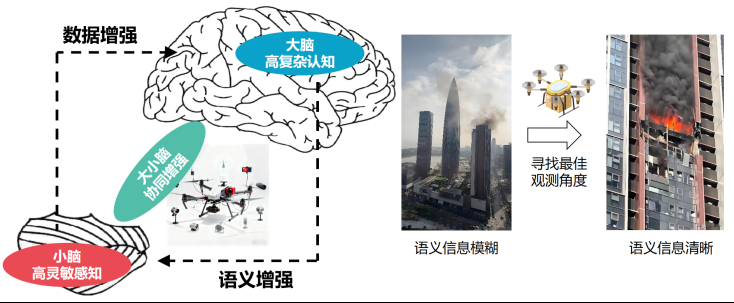
\includegraphics[width=1.00\linewidth,height=0.82\textheight,keepaspectratio]{figures/fig01_overall_framework.png}
\caption{认知卸载启发的多层次推理总体框架：大小脑协同增强语义理解，并由无人系统按需获取高质量观测}
\label{fig:report-1}
\end{figure}

\subsection*{研究方法}
本节按照三个子创新方向说明技术路线。三类方法共享同一设计逻辑：首先识别任务中不同认知过程的输入、输出、调用频率和可验证条件；其次依据模型能力和过程结构配置承担主体；最后通过显式中间表示将各模块连接起来。对于可由几何、图结构、规则或优化可靠求解的过程进行外部卸载，对于必须依赖开放语义和跨模态知识的过程保留大模型推理，并通过按需触发限制其调用范围。

这种方法与传统“级联多个网络”的区别在于，模块边界不是按照实现方便划分，而是按照认知性质划分。每个被卸载过程都应满足至少一个条件：其输入可以被结构化表达，其输出具有明确验证标准，或者其调用频率高到不适合持续使用高成本基础模型。反之，如果任务存在明显语义歧义、开放类别或需要跨场景知识，则保留基础模型的优势。下面分别从语义理解、空间认知和复杂系统规划三个层面展开。

\subsubsection*{快慢认知分流的复杂语义理解与按需推理}
\begin{figure}[htbp]
\centering
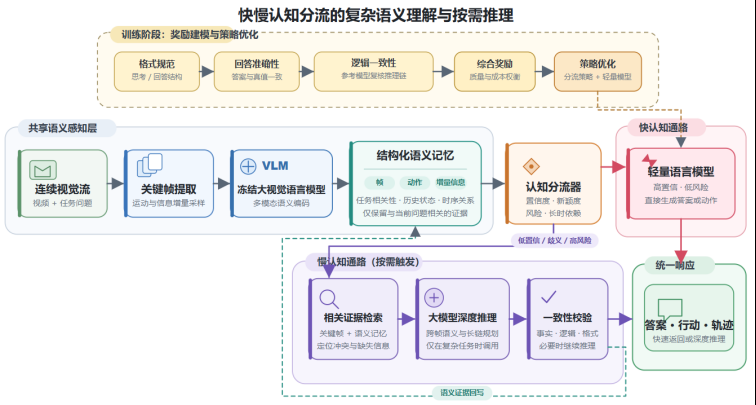
\includegraphics[width=1.00\linewidth,height=0.82\textheight,keepaspectratio]{figures/fig02_fast_slow.png}
\caption{快慢认知分流的复杂语义理解与按需推理技术路线}
\label{fig:report-2}
\end{figure}

（1）问题建模。连续具身视频同时包含大量重复帧、局部动作变化和跨帧空间关系。若直接把完整视频送入多模态大模型，不仅会造成视觉词元快速增长，而且会把“看见了什么”和“这些信息意味着什么”混合在一次端到端生成中。Embodied-R将任务拆为视觉语义感知和语言空间推理两部分：大规模视觉语言模型作为感知器，负责将视觉证据转化为语言可处理的语义；小规模语言模型作为推理器，负责基于这些语义完成关系组合、上下文整合和最终回答。

这种划分利用了两类模型不同的优势。大规模视觉语言模型具有更强的开放对象识别和跨模态描述能力，但重复调用代价高；小规模语言模型视觉能力有限，却可以在结构化文本空间中以更低成本进行多步推理。因此，系统不要求小模型重新学习通用视觉感知，也不要求大模型在每个问题上承担完整逻辑链，而是在两者之间建立稳定的语义接口。

（2）关键帧选择。视频相邻帧通常存在大面积重叠，尤其在机器人平移速度较低时，连续输入会重复编码同一墙面、道路或目标。关键帧模块首先从局部图像特征出发判断视野变化程度，通过特征点匹配和几何一致性估计相邻候选帧之间的重叠关系。当画面变化超过阈值时保留新帧，否则跳过高度重复的图像并继续向后比较。这样可以在不依赖任务标签的情况下把长视频压缩为具有代表性的视觉序列。

关键帧选择并不是固定间隔采样。固定间隔在匀速直线运动中可能足够，但在快速旋转、进入新房间或遮挡突然解除时容易遗漏决定性视角。基于视觉重叠的选择能够使采样频率随环境变化自适应：视野变化小时保留更少帧，视角旋转或新对象出现时自动提高保留密度。由此，输入压缩与空间信息变化建立直接联系，而不是简单追求最少帧数。

（3）增量语义表征。对于第一张关键帧，感知模型主要提取场景中的对象、属性及其相对空间位置；对于后续相邻关键帧，则重点描述三类增量信息：智能体发生了什么动作，前后帧之间哪些空间关系发生变化，以及有哪些新出现或与问题直接相关的对象。相比逐帧生成完整自然语言描述，这种增量表征把稳定背景信息和真正变化的信息区分开，使推理器可以更清楚地追踪“状态如何演化”。

该设计还解决了长视频中语义重复的问题。如果每一帧都重新描述全部对象，文本长度仍会随帧数线性增长；而增量描述只记录变化项，可以把连续视觉序列转换为较短的事件链。例如，模型不需要在每一帧都重复“桌子位于左侧”，只需在关系改变时记录“转向后桌子从左侧移动到后方”。这种表达更接近空间推理所需的状态转移，而非单纯图像字幕。

（4）大小模型协作。大模型的职责被限制为稳定的跨模态语义抽取，不直接参与每一步最终答案生成；小模型接收语义序列和问题，通过语言推理完成空间关系判断。这样可以冻结视觉语言感知器，把主要训练资源集中于参数规模更小的推理器。一方面保留大模型的开放词汇感知能力，另一方面避免对大规模视觉模型进行昂贵的端到端强化学习。

（5）强化学习驱动的慢思考。轻量推理器采用“先思考、后回答”的输出结构，并通过组相对策略优化学习具身空间推理。奖励由格式、答案准确性和思考—答案逻辑一致性共同构成。格式奖励保证模型显式区分分析过程与最终结论；准确性奖励保证任务目标不被形式约束取代；逻辑一致性奖励则检查分析过程是否真正支持最终答案，防止模型只猜中答案却形成与答案矛盾的推理链。

引入逻辑一致性约束具有重要意义。在只有答案奖励时，强化学习可能出现奖励投机：模型发现某些答案模式更容易得分，却没有形成稳定的空间关系推理。通过同时评价“结论是否正确”和“推理是否能推出结论”，训练目标从结果匹配扩展到过程一致。最终，小模型逐步形成对象枚举、关系分解、跨帧整合和结论复核等慢思考模式。

（6）按需触发与能力边界。快通道负责目标感知、状态判断、关键帧筛选和短程语义更新；当问题只依赖当前场景的简单事实时，可以直接利用已有语义快速回答。当问题涉及跨帧比较、遮挡关系、相对距离、视角变化或多步空间约束时，再触发慢通道执行更完整的推理。工程实现中还可以根据问题类型、语义不确定性和历史回答置信度设置触发条件，使推理深度与任务难度匹配。

（7）可检查接口。结构化语义序列不仅是压缩载体，也是错误诊断接口。当最终回答错误时，可以依次检查关键帧是否覆盖关键证据、视觉语言模型是否正确抽取对象与关系、小模型是否在关系组合阶段发生逻辑错误。与端到端视觉问答相比，这种接口使感知错误和推理错误能够被区分，为后续增加置信度估计、二次观察或回退到大模型提供明确依据。



（8）视觉变化驱动的帧级信息控制。Embodied-R中关键帧机制的核心并非简单追求更低采样率，而是以相邻观测之间的信息变化作为保留依据。机器人在连续运动时，视觉输入可以近似看作随位姿连续变化的观测流；当相邻画面具有较高重叠时，重复编码不会显著增加空间关系证据。系统通过局部特征与描述子的匹配判断视觉重叠，并在变化达到一定程度后接受新的关键帧。其作用相当于在视觉层建立事件触发机制：只有环境证据发生足够变化，才产生新的高层语义输入。

这一机制与后续语义差分形成配合。如果关键帧过密，即使语义模块只描述变化，仍会产生大量微小、无意义的状态更新；如果关键帧过稀，又可能把一次转向或遮挡解除前后的多个关系变化压缩到同一步中，增加推理困难。因此，帧级筛选的目标不是最小化帧数，而是在“证据完整性”和“输入冗余”之间寻找稳定工作点。实验中关键帧数量下降但准确率没有降低，说明筛选主要去除了重复观察，而没有系统性删除推理所需的关键变化。

（9）面向推理的语义差分。对后续关键帧同时输入前一关键帧和当前关键帧，使视觉语言模型能够直接比较两个时刻，而不是分别生成两段完整字幕再由语言模型自行寻找差异。其输出被约束为动作、空间信息变化和问题相关内容三部分。动作描述反映智能体自身运动，空间信息变化反映对象相对位置的改变或新对象出现，问题相关内容则对当前任务证据进行筛选。三类信息共同构成一个面向推理的状态转移描述。

这种表示比通用视频字幕更适合空间推理。通用字幕往往强调画面中显著对象，但不一定描述“对象从左侧变到后方”“机器人刚刚右转”“目标物首次进入视野”等对空间关系至关重要的变化。通过明确要求差分语义，感知模型的输出格式被任务结构约束，高层推理器不需要从冗长描述中重新识别状态转移。换言之，认知卸载不仅减少了输入，还改变了输入的组织方式，使每个语义片段对应一个可解释的空间事件。

（10）历史语义的递增整合。随着关键帧依次到来，系统形成语义序列，而不是一次性把所有图像送入模型。新的语义项可以与已有历史共同输入轻量推理器，因而长视频被转化为逐步扩展的结构化上下文。这种递增方式更符合机器人在线运行：系统不必等待视频结束后再进行推理，而可以在每次获得新关键证据时更新对环境的理解。对于未来实时部署，还可以进一步设置语义缓存，只保留仍与当前问题相关的历史关系，继续控制文本长度。

（11）GRPO在轻量推理器中的作用。小规模语言模型并不是通过传统监督学习简单模仿一段固定思维链，而是通过组相对策略优化在多个候选输出之间学习相对优势。对于同一个问题和语义输入，模型产生一组不同响应，再根据奖励比较这些响应的格式、答案和逻辑一致性。相对评价能够减少对额外价值模型的依赖，也更适合答案具有明确判定标准的多项选择空间推理任务。模型更新因此直接围绕“哪类推理过程更可能得到正确且一致的答案”展开。

（12）分阶段奖励调度。训练并非从第一轮就同时给予三类奖励相同权重，而是采用逐步递进策略。早期阶段首先强化“思考—答案”的输出结构，使模型稳定学会按照可解析格式组织响应；中间阶段提高答案准确性权重，防止模型只学会形式而缺少正确推理；后期再加入逻辑一致性要求，使模型在已经能够稳定回答的基础上修正思维链与结论之间的矛盾。这种课程式训练避免多个目标在训练初期相互干扰，也解释了为什么模型最终能够形成相对稳定的慢思考模式。

训练早期优先建立格式还有一个工程原因：若输出结构不稳定，自动答案提取和奖励计算本身就容易出现误判。先让模型形成固定的思考区和答案区，可以使后续准确性奖励更可靠。随后再提高准确性与一致性要求，训练信号由“是否按要求回答”逐渐转向“回答是否正确、推理是否可信”。这种顺序体现了从行为规范到任务能力再到过程质量的逐层塑造。

（13）逻辑一致性奖励对奖励投机的抑制。空间关系多项选择题的候选答案数量有限，仅使用最终答案正确性奖励时，模型可能在推理过程错误的情况下偶然猜中正确选项。若这种样本同样获得高奖励，模型会学到“答案正确即可”，而不需要保持推理链可信。逻辑一致性奖励通过额外检查思考过程与答案之间的语义关系，把偶然猜中的响应与真正能够支持结论的响应区分开。其价值因此不仅是提高可读性，更是改变强化学习优化方向。

（14）为什么不直接在小型视觉语言模型上强化学习。直接训练同规模视觉语言模型看似可以省去感知—推理接口，但实验表明其上限受到视觉感知能力约束。在相近训练条件下，直接对3B视觉语言模型进行强化学习的结果低于“强VLM感知加3B语言模型推理”的协作方式。原因是空间推理必须建立在可靠感知之上，小型视觉语言模型同时需要承担对象识别和推理，有限容量被两个能力共同占用。分工后，大型感知器保持冻结，小模型可以把参数和训练信号集中用于推理。

（15）推理长度与任务性质的适配。强化学习后模型并没有无限增长思维链，而是逐渐收敛到适合空间任务的响应长度。空间关系问题虽然需要多步整合，但通常不需要像复杂数学证明那样生成极长推导。过长响应反而可能重复已有关系或引入新的错误。训练过程中响应长度趋于稳定，说明慢思考的关键不是“写得越长越好”，而是形成足够完成对象枚举、关系组合和结论检查的紧凑推理过程。这一点对于边缘部署同样重要，因为输出词元数量也直接影响生成时延。

（16）分布外泛化。训练集主要来自室内第一视角和城市无人机视频，但进一步在不同内容和场景特征的数据上测试模型，可以判断它学到的是任务模板还是更一般的空间推理策略。实验显示，强化学习后的轻量模型在分布外任务上仍具有较好的迁移能力，而监督微调在部分数据上出现退化。这表明通过奖励学习形成的分析行为并不完全依赖训练集中固定的语言形式，对于新场景中的空间关系仍可以复用。

（17）面向在线系统的回退策略。由上述机制可以进一步得到一个适合工程部署的分层触发方案：正常情况下由关键帧提取和轻量推理器完成高频问题；当感知语义置信度不足、候选答案差异很小、推理输出格式异常或逻辑一致性低时，再调用更强的大模型重新检查。这样，大模型从默认必经路径变为困难样本的后备能力。虽然当前实验主要验证协作框架本身，但这一扩展与认知卸载原则一致，可以进一步把平均计算量与最坏情况能力分离。

（18）感知错误与推理错误的责任分解。若最终空间答案错误，可以沿接口逆向分析：首先确认决定性视觉变化是否被关键帧保留；其次检查VLM是否正确描述动作、对象关系和问题相关内容；最后检查轻量模型是否在语义条件正确时仍作出错误组合。三步分别对应数据选择、跨模态感知和语言推理。这样的诊断比直接观察端到端视频问答输出更具有操作性，也使后续实验能够针对真正薄弱环节设计，而不是通过增加模型规模笼统补偿所有错误。



（19）感知输出的任务相关裁剪。结构化语义并不是把视觉内容完整转写成文本，而是围绕当前空间问题只保留能够改变判断的证据。对于已经稳定存在且与问题无关的背景对象，不需要在每个关键帧中重复记录；对于问题涉及的地标、相对方向、遮挡关系和自身运动，则需要持续维护。这样，感知模块输出的语义序列具有“状态变量”而非“视频字幕”的性质：每一项都应当能够解释为什么后续空间判断发生变化。该设计进一步减少视觉冗余向文本侧迁移，避免出现图像帧已经压缩、但自然语言描述仍然线性增长的问题。

（20）证据链与推理链的分离。系统把视觉证据链和语言推理链保持为两个不同层次。前者记录“观察到了什么变化”，后者回答“这些变化共同意味着什么”。当模型回答相对方位、距离变化或遮挡关系时，轻量推理器只需要引用已经结构化的证据，而无需重新解释原始画面。由此，推理长度主要由关系组合复杂度决定，而不再直接由视频时长决定。对于长时程具身任务，这一点可以显著减缓上下文随时间膨胀，使模型能够把计算集中在少量真正影响答案的空间事件上。

（21）训练阶段与部署阶段的职责一致性。训练时，轻量语言模型始终接收与部署阶段同类型的结构化语义，而不是依赖训练阶段额外提供的人工标注信息。这样可以避免训练—部署接口不一致导致的性能落差。强化学习优化的是“给定感知语义后如何推理”，大规模视觉语言模型则保持相对稳定的感知职责。由于两部分可以独立更新，后续若更换更强的视觉感知器，只要保持语义接口格式一致，推理模块不需要从头训练；反之，也可以在不重新编码全部视频的情况下继续优化轻量推理器。

（22）按需推理的运行逻辑。从系统角度，快慢分流可以进一步表示为一个事件驱动的状态机。连续观测首先经过关键帧与语义变化检测；若新增信息仅更新已知对象的局部状态，系统维持快速通道；当出现新的关键对象、关系冲突、跨帧比较需求或当前答案置信度下降时，再进入慢推理。慢推理完成后，其结论被重新写入结构化状态，供后续快速周期复用。该逻辑使高成本推理从固定周期调用转变为由信息增量触发，形成“视觉变化决定是否更新语义、语义变化决定是否启动深推理”的两级触发链。

（23）错误隔离与回退。由于关键帧、视觉语义和语言推理之间存在显式接口，系统可以为每一级设置独立的异常条件。关键帧覆盖不足时可回看邻近帧，视觉语义存在冲突时可重新调用感知模型，轻量推理器输出不一致时则可提升到更强模型复核。与端到端模型只能重新运行整条链路相比，这种局部回退可以把额外计算集中在发生不确定性的环节。其工程意义在于，系统既可以维持大多数简单样本的低成本处理，又保留困难样本调用更强能力的通道。

\begin{figure}[htbp]
\centering
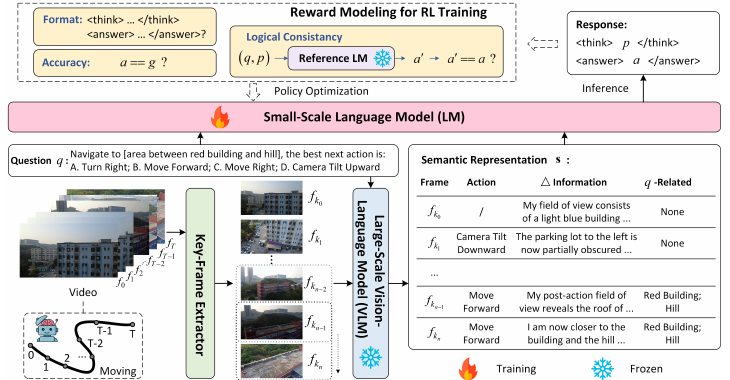
\includegraphics[width=1.00\linewidth,height=0.82\textheight,keepaspectratio]{figures/fig03_embodied_framework.png}
\caption{Embodied-R大小模型协同推理框架：视觉语言模型负责关键帧语义抽取，小规模语言模型负责强化学习驱动的空间推理}
\label{fig:report-3}
\end{figure}

总体来看，该方向的关键并不是“小模型替代大模型”，而是让两个模型分别承担适合自身的认知过程。视觉感知保持开放性，空间推理获得专门化，关键帧与增量语义控制输入规模，强化学习则让轻量模型具有更加稳定的审慎推理能力。由此形成从视觉压缩、语义抽取到语言推理的连续认知卸载链条。

\subsubsection*{全局—局部空间分解的复杂空间认知与记忆规划}
\begin{figure}[htbp]
\centering
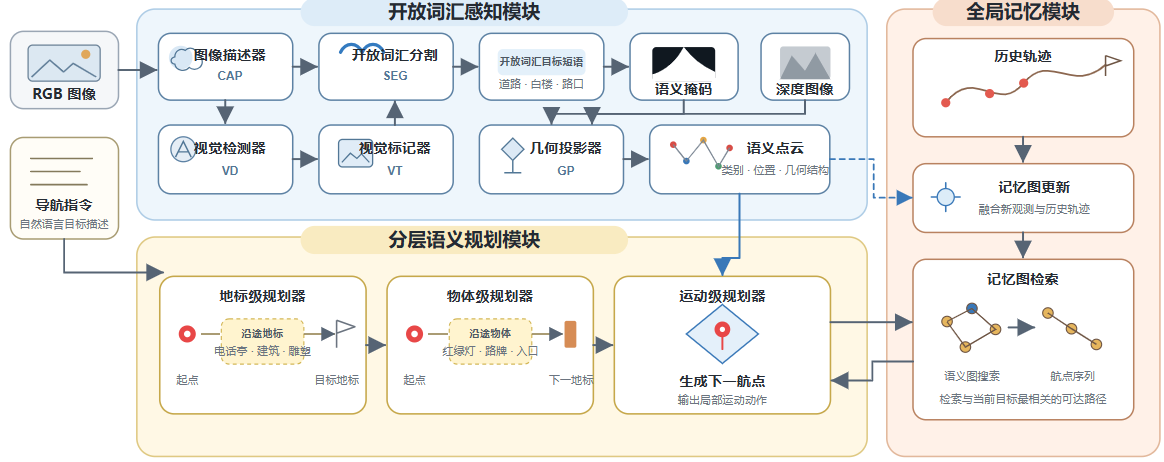
\includegraphics[width=1.00\linewidth,height=0.82\textheight,keepaspectratio]{figures/fig04_city_custom.png}
\caption{开放词汇感知、分层语义规划与全局记忆协同框架}
\label{fig:report-4}
\end{figure}

（1）城市空中导航的空间表示。CityNavAgent面向连续城市环境中的空中视觉—语言导航。与室内离散节点导航不同，城市无人机具有连续三维运动空间，单个自然语言指令可能跨越道路、建筑、交叉口和设施等多个尺度。系统首先利用开放词汇感知模块从全景RGB图像中生成对象描述，并利用开放词汇检测和分割获得对应视觉区域；再结合深度和机器人位姿，把二维对象投影到三维度量空间，形成局部语义点云。

语义点云承担从自然语言到可执行坐标的桥梁作用。仅依赖图像字幕可以知道“前方有一栋红色建筑”，但规划器仍不知道该建筑位于机器人坐标系中的具体方向和距离；仅依赖几何点云则缺少“哪一栋建筑与指令有关”的语义。将对象标签与三维坐标绑定后，高层语言规划输出的地标或对象可以直接映射为局部空间目标，使语义推理不再停留在文本层面。

（2）地标级子目标分解。系统首先由语言模型解析完整指令，提取按照任务顺序出现的地标序列。长距离目标由此被分解为若干阶段任务，例如先沿道路前进到交叉口，再接近某类建筑，最后在目标设施附近搜索。地标级规划只回答“下一阶段应该到达哪个语义区域”，不直接生成细粒度飞行动作，从而把长程语言理解与短程控制解耦。

这种分解能够降低连续动作空间的搜索难度。若无人机直接从起点预测最终航点，微小方向误差会在长距离上不断累积，且语言中间地标无法发挥约束作用。按地标推进后，每个阶段都可以利用新的局部观测校正后续目标，形成“语言指令提供全局顺序、实时视觉提供局部证据”的闭环。

（3）物体级语义推理。当目标地标尚未直接出现在视野中时，系统并不要求语言模型凭空预测其三维坐标，而是推理当前可见场景中最可能通向该目标的对象区域。例如，当任务要求寻找交通设施时，道路、路口等可见对象可以作为更合理的中间区域。物体级规划根据完整指令、当前子目标和场景描述生成一组候选对象，并按照语义相关性排序，再将最相关对象映射到语义点云。

保留候选对象而非直接产生连续动作具有两层作用。第一，高层语言推理只需判断语义关联，不承担几何计算；第二，当最优候选缺失或感知置信度不足时，系统仍可利用次级候选进行替代，而无需重新解释整个长指令。这种候选机制为后续引入不确定性和回退策略提供了天然接口。

（4）运动级规划。确定语义目标后，系统从对应语义点云中得到可度量三维位置，将其转化为下一航点并分解为无人机能够执行的局部运动。运动层只负责“如何到达已经确定的局部目标”，不再处理长程语言语义。因此，地标级、物体级和运动级三个层次分别对应战略方向、局部语义区域和即时空间动作，避免一个模型同时跨越多个空间尺度进行推理。

（5）全局拓扑记忆。仅有层次化规划仍无法解决长期历史遗忘。CityNavAgent将成功历史轨迹、关键位置和视觉观测存入三维拓扑图。节点记录航点坐标及其观察，边记录相邻节点之间的可达关系和距离。新的成功轨迹可以与已有图增量融合，使重复经过的区域逐渐形成更完整的城市级记忆。对于没有成功到达目标的路径，则不直接写入长期记忆，以降低错误路径对后续导航的污染。

该记忆与把全部视频写入上下文有本质差异。拓扑图只保留对导航具有长期价值的结构关系，例如“两个位置相连”和“某节点附近曾观察到什么”，而不是保存每一帧原始像素。当新任务进入已访问区域时，系统可以先在记忆图中检索与当前地标序列相关的节点，通过图搜索复用已有可达路径，从而把长时程记忆从大模型上下文外化为稳定的数据结构。

（6）记忆检索与裁剪。随着长期运行，拓扑图本身也会增大，因此系统并非每次都对完整图执行搜索，而是优先抽取当前位置附近的局部子图，再根据语义相关性和空间冗余进行筛选。只有与当前指令和剩余地标相关的节点进入规划范围。这样，全局记忆虽然可以长期累积，但单次决策仍保持有限规模，实现“记忆容量”和“即时计算量”的解耦。

（7）未知空间探索中的骨架图。SCOPE进一步研究没有语言目标时的自主探索。完整三维占据地图包含大量体素，而真正决定不同区域可达性的结构通常集中在自由空间主干。系统从距离场中增量提取骨架节点，并根据距离、碰撞检查和几何条件建立连边。地图更新时，只在受影响的局部包围盒内维护骨架，而不是重建整个图，从而持续获得紧凑的自由空间拓扑。

前沿点被关联到附近骨架节点，使骨架不仅表达已知空间连通性，还能够指示“哪些主干节点连接着尚未探索的区域”。这一步把数量庞大的前沿点进一步聚合到更少的结构节点上。规划器不再直接面对整个体素地图和全部前沿，而可以在骨架层面计算区域间的近似路径距离和跳数关系。

（8）隐式未知区域建模。仅知道前沿位置仍不足以判断其背后未知空间的规模。SCOPE从前沿簇附近生成几何探针，沿多个方向估计进入未知空间后的潜在延伸深度，并根据探针交叠和空间邻近关系，把相关骨架节点聚合为隐式未知区域。这里的“隐式”意味着系统不需要预先恢复未知空间的完整几何，只保留用于判断区域规模、方向和相互关系的必要信息。

这种表示特别适合探索问题，因为未知空间本身没有真实地图，过度精细建模既不可靠也昂贵。几何探针提供的是对“前方可能还有多深、多大区域”的结构估计，用于战略层选择即可；真正进入区域后，再由实时传感器更新地图。由此形成“粗粒度未知区域用于全局排序、精细局部地图用于即时避障”的双尺度表示。

（9）高频近端规划。正常运行时，近端规划器优先在当前位置附近选择可达、平滑且能够继续获取信息的目标。候选节点根据骨架跳数、传感范围和当前运动状态筛选，代价不仅考虑路径长度，还考虑速度调整、转向和高度变化等实际飞行因素。因此，局部目标并非单纯选择欧氏距离最近的前沿，而是选择能够以较低运动代价持续推进探索的视点。

近端规划的意义在于把绝大多数规划周期限制在局部范围。地图每次更新都会产生少量新前沿，但只要附近仍有合理目标，系统无需重新求解所有区域的全局访问顺序。这能够减少全局序列因前沿轻微变化而反复重排，也使无人机轨迹更连续，避免为了追求瞬时全局最优而频繁大角度转向。

（10）按需区域序列规划。只有当当前位置附近缺少有效目标时，系统才调用区域序列规划器。该规划器以隐式未知区域为节点，利用骨架图中的最短路径距离近似跨区域移动代价，并优化后续访问顺序。由于调用发生在局部探索无法继续推进的时刻，全局组合优化从“固定频率周期执行”转变为“由系统状态触发”。

在这一机制下，全局层负责决定“下一片值得转移到的区域”，局部层负责“如何连续、平滑地探索当前区域”。全局规划可以接受一定程度的粗粒度近似，因为真正的障碍和运动约束仍由局部规划处理；局部规划也无需承担长期最优性，因为当区域即将耗尽时会重新获得全局方向。两层之间形成互补，而不是互相替代。



（11）开放词汇感知的逐级落地。CityNavAgent并不是直接要求语言模型从全景图像生成一个三维航点，而是先完成对象描述、目标检测、精细分割和三维投影。图像描述器负责发现开放类别对象，检测器利用文字标签确定对象区域，分割器获得更精确掩码，最后结合深度与相机位姿恢复世界坐标。每一步都缩小从“自然语言对象”到“可执行位置”的表示差距，使高层规划可以在语义与几何对齐的地图上工作。

这种处理尤其适合城市环境。道路、建筑、交通灯、车辆和公共设施种类远多于封闭室内数据集，预先定义有限类别容易遗漏导航指令中的关键对象；另一方面，纯视觉语言描述又缺少度量坐标。开放词汇检测与三维投影结合后，系统既不需要为每一类城市对象重新训练封闭分类器，也不需要让语言模型猜测空间距离。语义开放性和几何确定性分别由不同模块提供。

（12）地标序列作为任务进度变量。长自然语言指令中不仅包含终点，还包含沿途地标及顺序关系。将其解析为地标序列后，系统能够显式记录当前已完成到哪一个阶段。任务进度不再隐含在长文本和历史动作中，而成为可更新的状态变量。当某个地标被确认到达后，规划器只需关注剩余序列；当导航发生偏离时，也可以判断偏离发生在哪个阶段。这种状态外化对长程任务尤为重要，因为它减少模型重复读取已经完成指令的需求。

（13）OROI候选与常识推理。物体级规划处理的是一个典型的“目标不可见但存在语义线索”的问题。系统没有要求模型直接预测不可见地标，而是从当前已观察对象中列出最可能与下一地标关联的若干区域，并按概率排序。例如，交通灯暂时不可见时，道路或路口比建筑立面更值得接近。这里大模型的优势被限定在常识语义关联，而不是距离计算或航迹控制。候选集合进一步提供冗余，使第一选择不可靠时仍有备选方向。

（14）语义点云中的航点生成。得到OROI后，运动级规划器在语义点云中找到具有相同语义标签的三维点，并通过其空间分布计算局部目标。高层语言输出因此不直接成为控制命令，而先经过三维地图映射。随后局部路径再分解为机器人可执行动作。通过这一过程，可以明确区分“语义上应该去道路区域”和“物理上应该到达哪个三维坐标”，避免语言模型自行完成连续空间插值。

（15）记忆图的有效性控制。CityNavAgent只将成功到达目标的历史轨迹并入全局记忆，而不是无条件保存所有走过的路径。这一设计降低了失败轨迹、错误地标和盲目探索污染长期记忆的风险。历史轨迹被表示为带坐标和视觉观测的节点以及相邻路径距离构成的边，新轨迹与已有图之间若存在足够近的节点，还会建立新的连接。随着多次任务执行，图结构逐渐从独立轨迹集合演化为可以跨任务复用的城市局部拓扑。

（16）记忆图搜索对动作空间的压缩。当机器人到达记忆图中的已知节点且剩余目标与历史路径相关时，可以直接在图上搜索到目标附近的节点序列，而不是继续随机探索或让大模型每一步重新选择方向。原本连续三维空间中的大量动作候选被缩减为一条由已验证节点构成的路径。这里的认知卸载不是降低环境复杂度本身，而是利用过去经验把“再次求解”转化为“检索并复用”，体现长期记忆的计算价值。

（17）为什么室内航点预测难以直接迁移到城市空中导航。传统连续VLN方法往往基于室内环境训练二维或近二维航点生成器，而城市无人机具有更大的空间尺度和明显高度自由度。实验对比显示，室内方法预测的航点在户外与参考航点距离显著增大。原因一是尺度差异使固定局部预测范围不足，原因二是三维运动中的高度选择不能被二维候选充分表达。CityNavAgent采用语义对象和三维投影替代直接复用室内航点网络，体现了“任务结构改变时，应重新设计外部表示，而不是强行迁移原有模型”的思想。

（18）SCOPE中的增量骨架维护。自主探索地图会持续扩大，若每次更新都重新计算完整Voronoi或全局拓扑，计算量随地图规模不断增长。SCOPE只在新观测影响的局部范围更新骨架节点和连边，并保留未受影响区域的已有结构。骨架节点位于自由空间具有代表性的主干位置，可用于近似路径距离和区域连接。增量维护使长期运行中的拓扑更新成本主要与新观测局部变化相关，而不是与全部已知地图成比例。

（19）激活节点与前沿关联。并不是所有骨架节点都同等重要，只有与当前未知区域和候选视点相关的节点才进入更高层规划。系统把前沿及其可观测候选与骨架连接，从而形成“已知自由空间主干—前沿入口—未知区域”的关系。这样，大量局部前沿点被聚合到较少的拓扑入口，区域序列规划器不需要对每个原始前沿单独排序，显著降低全局问题维度。

（20）几何探针对未知空间的近似。对于尚未真正观测的区域，系统无法知道完整形状，但可以从前沿沿可行方向发射探针，估计未知空间可能延伸的深度。多个探针共同提供区域规模和独立程度的粗略信息。该估计不追求重建未知空间，而只回答全局决策所需的问题：某个入口背后是否可能存在足够大的未探索区域、不同入口是否实际上指向同一片空间。对战略排序而言，这类近似信息已经足够。

（21）隐式区域聚类减少重复战略目标。若两个骨架入口的探针大范围重叠，它们很可能通向同一个未知区域；若直接把二者作为独立目标，全局规划器可能重复安排访问。SCOPE根据探针关系和空间邻近性聚类激活节点，把多个入口合并为一个隐式区域。规划对象由大量前沿点进一步压缩为少量区域，从而把全局序列规划的组合规模控制在较低水平。

（22）近端规划中的运动学代价。局部规划并非只考虑信息增益，还综合当前速度、转向和高度变化等运动代价。无人机如果为了追逐一个略高信息增益的前沿频繁反向或急转，实际飞行时间和能耗会增加。把运动平滑性纳入近端目标选择后，系统优先延续当前运动趋势，在局部区域持续获取新信息。全局层只给出大方向，具体如何到达由局部运动学成本决定，这使两层职责更加清晰。

（23）区域序列规划的低频重计算。只有当近邻缺乏有效目标时，才说明当前局部区域接近探索完成，此时重新比较不同隐式区域的价值才有意义。区域序列规划器利用骨架最短路径近似跨区域代价，并在区域层求访问顺序。由于这些区域空间距离较远，局部短时运动学非对称对战略排序影响相对较小，可以用更简化的全局代价模型。全局得到的下一个战略区域随后交回近端规划器执行，实现战略与控制解耦。

（24）避免拓扑振荡。传统方法若对持续变化的全部前沿频繁求全局顺序，一个前沿新增或消失就可能导致最优序列改变，使机器人在多个方向间反复切换。SCOPE通过局部连续推进和低频区域级重规划，降低这种拓扑振荡。当局部仍有可探索空间时不轻易改变战略方向，只有局部耗尽才转移区域。实验中轨迹更平滑、平均速度更稳定，与这一机制相符。

（25）两类空间认知工作的统一接口。CityNavAgent的高层状态是语言地标与历史路径，SCOPE的高层状态是隐式未知区域与骨架连接。二者虽然一个以语义为核心、一个以几何为核心，但都把大规模连续空间压缩成有限的节点或阶段状态。局部执行层不需要理解全部全局信息，只接收当前目标；全局层也不需要处理每次控制细节，只在目标失效或阶段完成时更新。该共性说明“全局低频状态—局部高频动作”可以作为不同城市机器人任务共享的空间认知架构。



（26）记忆图的在线更新与路径复用。全局记忆不是一次性离线构建的静态地图，而是随着成功导航轨迹逐步扩展。每完成一段可验证路径，系统将新的关键航点及其视觉观测写入当前轨迹图，并根据空间邻近关系寻找是否能够与历史图中的已有节点建立连接。当当前位置进入已知区域后，规划器优先在记忆图中搜索通往剩余地标的节点序列；只有记忆无法覆盖当前任务时，才重新依赖开放词汇感知与语义推理探索未知区域。这样，系统把“已经解决过的空间问题”从重复推理转化为图检索，把大模型资源留给真正陌生的场景。

（27）语义候选与几何候选的双重筛选。物体级规划产生的OROI首先表达“哪些当前可见对象在语义上可能通向目标”，随后必须在三维语义点云中找到对应空间实体，才能成为可执行候选。若语言模型生成的对象在当前地图中不存在，则该候选不会直接转化为航点；若多个实例具有相同语义标签，则进一步利用位置、前进方向和阶段目标进行筛选。这一过程把大模型输出限制在环境中真实存在的候选集合内，降低开放语言生成与连续物理空间之间的错位。

（28）阶段完成与全局重规划触发。三级语义规划并不要求每个控制周期都重新解析完整语言指令。地标级状态在阶段完成前保持稳定，物体级目标可随着局部观测更新，而运动级航点以更高频率执行。当当前地标被确认到达、目标对象长期不可见、局部航点连续失败或记忆路径与新观测冲突时，系统才回到更高层重新选择地标或候选区域。由此，不同层级具有不同的更新频率，语言推理、语义地图和局部控制之间形成与空间尺度一致的时间尺度分离。

（29）SCOPE中的局部—全局状态切换。近端规划器持续检查当前位置附近的活跃骨架节点和可观测前沿，只要局部仍存在可行且具有探索价值的候选，就保持局部推进；当近邻候选被消耗、被判定不可达或信息增益不足时，才将当前状态提升到区域序列层。区域层完成下一隐式未知区域选择后，系统重新下降到近端规划。该切换机制避免在同一局部区域内反复求解全局访问序列，使高成本组合优化真正只承担战略转移功能。

（30）地图增量与规划增量的一致性。SCOPE不仅在规划层采用按需更新，骨架结构本身也围绕局部地图变化增量维护。新传感数据只影响当前观测附近的自由空间和前沿，未变化区域的骨架节点与连边可以继续复用。因此，地图增长不会迫使系统每次从零构建全局拓扑。规划器读取的是持续演化的紧凑骨架，而不是完整体素地图，长期运行时计算量更多取决于新观测引起的局部变化，而不是全部历史空间规模。

（31）两类空间任务的统一状态表达。CityNavAgent和SCOPE虽然分别以语言地标和未知区域为高层对象，但都可以抽象为“全局状态节点、局部可执行目标和事件触发更新”三部分。语言导航中的全局节点是地标与记忆位置，自主探索中的全局节点是骨架区域；前者通过语义完成状态转移，后者通过前沿耗尽完成状态转移。统一视角说明，复杂空间认知的关键并不是某一种特定地图，而是把连续空间中长期有效的关系压缩成低频状态，把短时间内快速变化的运动问题留给局部层处理。

\begin{figure}[htbp]
\centering
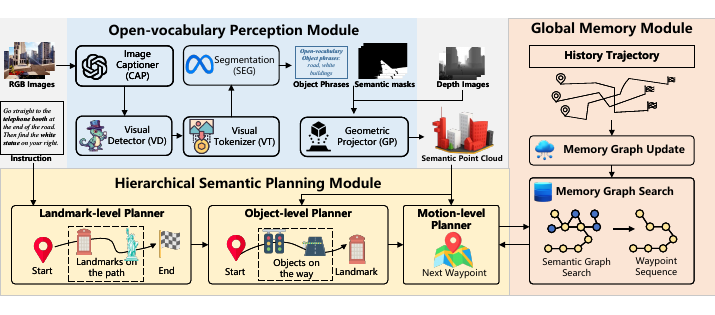
\includegraphics[width=1.00\linewidth,height=0.82\textheight,keepaspectratio]{figures/fig05_city_framework.png}
\caption{CityNavAgent三级语义规划与全局记忆框架}
\label{fig:report-5}
\end{figure}

\begin{figure}[htbp]
\centering
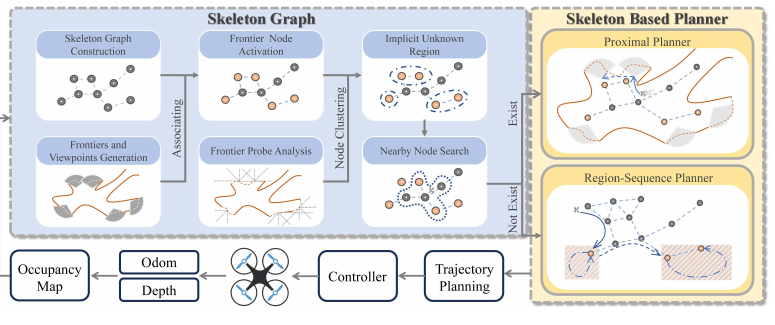
\includegraphics[width=1.00\linewidth,height=0.82\textheight,keepaspectratio]{figures/fig06_scope_framework.png}
\caption{SCOPE骨架图维护、隐式未知区域分析与按需层次规划框架}
\label{fig:report-6}
\end{figure}

CityNavAgent与SCOPE分别处理“有语言目标的城市导航”和“无先验地图的自主探索”，但二者采用一致的认知卸载逻辑。CityNavAgent把长期语言指令外化为层次化子目标，并把历史空间知识外化为拓扑记忆；SCOPE把大规模未知空间外化为骨架与隐式区域，并把高成本全局排序限制为低频事件。二者共同说明，复杂空间认知并不要求每一时刻维持完整全局推理，而可以通过紧凑的长期结构和高频局部反应实现更稳定的长时程运行。

\subsubsection*{高阶认知—灵敏执行协同的复杂系统规划}
（1）异构空地搜索中的认知拆分。在多无人机—无人车协同搜索中，端到端大模型通常需要同时解释用户意图、判断目标位置、验证飞行与地面运动约束、生成动作并分配任务。随着智能体数量增加，所有观测被拼接进同一上下文，语言模型既承担不擅长的物理推理，又成为所有智能体同步等待的中心瓶颈。该问题不是简单增加模型参数能够解决的，因为物理可行性与组合分配本身具有更适合显式求解的结构。

CAU方法首先把复杂协同任务中的认知过程区分为三类：高阶语义认知、具身物理认知和群体协调认知。高阶语义认知回答“任务是否已经完成”“哪些场景要素与任务有关”“哪类智能体更适合该子任务”；具身物理认知回答“某个平台能否执行某动作”“该目标是否可达”“路径是否违反障碍或禁飞约束”；群体协调认知则回答“多个可行行为之间应如何组合，避免不同主体重复或冲突”。

（2）认知感知单元。系统将一个可执行行为表示为由智能体、动作、目标和子任务组成的认知感知单元。四类要素分别对应“谁来做、做什么、朝哪里做、为了完成什么”。与自然语言行为描述不同，每个要素都可以与具体的物理或任务属性关联，使“无人机搜索目标区域”进一步落实为特定平台、候选动作、空间目标和任务状态之间的结构化关系。

构建单元时，系统首先检查子任务与智能体类型是否兼容，例如只有具备相应感知范围或运动能力的平台才保留为候选；随后计算任务与空间目标的语义相关性，并过滤已经充分探索或与任务无关的区域；对于智能体和动作组合，再依据障碍、禁飞区、地面可通行性和运动限制判断执行可能性；最后结合动作到目标的物理距离形成综合评价。这样，语言模型不再需要在自然语言中隐式“想象”一条动作是否可行。

（3）大模型语义职责收缩。CAU框架中的大模型只承担少量难以被固定规则替代的语义判断，例如从自然语言任务和视觉描述中识别任务完成状态、判断环境要素与目标之间的语义相关性，以及推荐更适合某类任务的平台。其余可以由距离、地图、能力表或约束函数确定的过程全部外部化。大模型输出因此从长动作序列缩减为少量结构化变量，降低输入输出词元规模，也减少生成错误传播到物理执行层的机会。

对于要素相关性判断，系统进一步采用先提取关键场景要素、再执行显式语义匹配的两阶段方式，而不是让大模型直接从长描述中自由生成相关区域。这样既保留语言模型理解“目标与环境之间弱语义关联”的能力，又用结构化候选集合限制幻觉范围。大模型负责“相关不相关”的开放语义，几何模块负责“能不能到”的确定性判断，两类证据不再混在同一输出中。

（4）CAU图协同。单个认知感知单元描述一条候选行为，多智能体协调则进一步表示为由智能体、动作、目标和任务四类节点组成的结构化图。一个满足约束的闭环对应一条完整可执行行为。候选边权综合考虑任务—目标相关性、任务—智能体兼容性、动作可执行性和物理距离，使“更相关、更适合、更可行且代价更低”的组合获得更高优先级。

系统在图上求解约束组合优化，而不是让多个语言智能体通过对话逐步达成一致。约束可以明确规定每个智能体在当前周期只选择一个动作、同一动作不能被多个主体无意义重复占用、动作必须指向有效目标且目标必须服务于具体任务。候选中的不兼容平台和不可执行动作会提前被剪枝，使组合搜索主要发生在已经具有物理意义的行为之间。

（5）异步执行机制。端到端集中式方案通常要求所有机器人完成当前动作并上传观测后再统一调用大模型，系统周期受到最慢主体限制。CAU架构把语义更新、图优化和机器人运动线程解耦，智能体完成局部动作后即可根据最新可行单元继续执行，不需要等待其他主体同步结束。中心图持续以较高频率维护候选关系，而大模型只在任务语义发生显著变化或需要重新解释环境时更新高层变量。

这种异步架构将“所有智能体等待一次大模型联合推理”的同步瓶颈转换为“各智能体只等待本地规划结果”的局部闭环。对于速度差异明显的无人机和无人车尤其重要：无人机可以快速完成大范围观察，无人车则以较低速度接近地面目标，两者无需强制共享相同动作周期。异构性由原来的系统负担转化为可以利用的能力差异。

（6）视觉词元冗余。复杂系统的另一类瓶颈来自视觉语言模型内部。以常见视觉语言架构为例，一张图像在进入语言模型后会被转换为数百甚至数千个视觉词元，这些词元在每一层参与注意力和多层感知机计算。高分辨率模型中，视觉词元数量可能远高于文本问题本身。若直接保留全部词元，即使外部系统已经减少大模型调用次数，单次视觉推理仍可能占据主要显存和时间。

（7）局部—全局平衡的词元重要性。Balanced Token Pruning指出，现有剪枝策略常只依据当前层注意力判断词元重要性。这种做法有利于保持当前层输出，却可能删除当前暂时不显著、但后续深层表示需要的互补视觉信息。另一类只强调词元多样性的策略虽然有助于保留全局覆盖，却可能忽略当前问题真正相关的局部区域。视觉词元剪枝因此被重新建模为当前层局部一致性与未来层全局表示之间的平衡问题。

具体而言，注意力相关性用于衡量某个视觉词元对当前语言输出的直接贡献，多样性则用于避免剩余词元集中在少数相似区域。两种目标在不同网络深度中的重要性并不相同。浅层被删除的词元会影响更多后续层，因此需要更谨慎地保护全局信息；随着网络加深，剩余计算层数减少，当前问题相关的注意力可以占更大权重。由此形成随层深变化的分阶段剪枝策略。

（8）校准驱动的剪枝层选择。并非所有解码层都适合执行词元删除。系统使用小规模校准集分析视觉表示和注意分配随网络深度的变化，选择信息发生明显重组且适合开始压缩的层级。校准只用于确定通用剪枝位置，不需要针对每个任务重新训练模型，也不改变原模型主体参数。这样可以避免采用固定等间隔剪枝造成的结构失配。

（9）高效词元选择。多样性计算若直接在全部词元之间进行两两比较，会产生额外二次复杂度，可能抵消剪枝节省的计算。因此，BTP利用图像词元原有的二维空间布局进行初始化，使代表性词元先覆盖不同空间区域，再结合注意力和多样性进行筛选。同时对注意力得分进行重新平衡，减轻位置编码等因素造成的系统偏置。其目标不是只减少理论FLOPs，而是让选择过程本身足够轻量，最终能够降低真实端到端时延。



（10）CAU的形式化行为链。CAU可以理解为把一次候选具身行为拆成任务、目标、智能体和动作四个相互约束的要素。一个候选只有在任务与目标具有语义关联、智能体具备执行该任务的能力、动作在当前环境中物理可行，并且动作能够把智能体有效引向目标时才具有完整意义。这种闭环结构使每条候选行为都可以逐项检查，而不是只依赖一段自然语言解释“为什么应该这样做”。

（11）语义相关性与物理可行性的分离。目标区域是否与任务有关，本质上可能依赖开放世界常识，例如“寻找受困人员”与道路、车辆、建筑入口之间存在弱语义关系；但机器人是否能到达目标，则可以由地图和运动约束判断。CAU把前者保留给大模型，把后者交给专用算法。即使语义模型给出一个看似合理的候选，只要几何验证失败，该候选也不会进入最终执行。这样可以阻断大模型错误直接传播为物理动作。

（12）两阶段语义匹配。面对复杂场景描述时，若直接要求大模型从全部视觉文本中输出唯一目标，容易受到无关对象和长上下文干扰。CAU相关流程先抽取任务可能关注的环境要素，再对有限候选进行相关性判断，相当于把开放生成问题转化为候选匹配问题。实验中两阶段方法的要素相关性准确性接近人工判断，说明减少搜索空间能够显著提高大模型在结构化任务中的稳定性。

（13）能力兼容约束。异构机器人最基础的差异是不同平台能够执行的任务和动作不同。CAU以显式兼容关系表达这种差异，而不是每次通过提示词提醒大模型“无人车不能飞、无人机不适合某些近地操作”。平台能力被写成可复用约束后，新任务到来时只需检查任务类型与能力关系；新增机器人时，也主要更新其能力和动作集合。系统因此获得比自然语言规则更稳定的可扩展接口。

（14）环境相关动作可行性。即使某个平台理论上拥有某个动作，该动作在当前环境中也可能不可执行。地面路径可能被障碍阻断，空中航迹可能穿过限制区域，目标也可能位于当前传感或运动范围之外。CAU将这些环境依赖因素纳入物理验证，使“平台有能力”与“此刻可以执行”成为两个不同判断。前者较稳定，后者随地图和状态在线更新，这使候选行为能够适应动态环境变化。

（15）距离与代价的定量化。候选行为完成语义和可行性过滤后，还需要比较哪个方案更值得执行。空间距离为不同候选提供可量化代价，使任务分配不只判断“能不能做”，还考虑“由谁做更合适”。对于无人机和无人车，由于运动方式不同，距离或运动代价可以采用平台对应的度量方式。大模型因此无需在语言中估计“哪个机器人更近”，而由可计算的物理量直接参与权重。

（16）CAU图从行为验证到群体组合。单个CAU保证一条行为链内部自洽，但多个机器人同时选择行为时还可能发生冲突，例如多个主体重复追踪同一目标，或者一个主体被分配多个互斥动作。CAU图把所有有效候选组织为智能体、动作、目标和任务构成的循环四部图，在图上选择满足全局约束的CAU组合。群体协调由此从多轮语言协商转化为确定性的组合优化。

（17）候选剪枝与规模控制。图优化理论上会随节点数量增加，但许多组合在进入求解器前就可以根据能力不兼容、动作不可行或低目标权重删除。任务一旦完成，相应节点和候选关系也可以动态移除。实验中的规模分析表明，在常见节点密度范围内规划延迟保持较低，说明结构化预筛选能够把实际求解问题限制在有效候选集合，而不是对全部可能组合暴力枚举。

（18）异步认知与异步运动。CAU系统并不是简单把同步规划器换成更快算法，而是重新组织多个线程的时序。机器人可以继续执行已经获得的局部任务，语义模块在需要时更新任务变量，CAU图则独立维护和求解当前候选。某个机器人完成动作后无需等待其他机器人，只要自身获得新的有效分配即可继续。这样，群体时钟从“所有机器人共同一步”转变为“每个机器人根据自身事件推进”，显著降低异构速度差异造成的空等。

（19）大模型输入的结构化压缩。端到端方案常把场景图像、每个机器人的位置、历史动作、路径约束和任务文本全部串入提示词，希望模型同时理解和计算。CAU框架只向大模型提供完成语义判断所需的信息，距离、可达性、平台能力和任务组合由外部模块维护。输入词元大幅减少的本质并不是文本摘要，而是把一整类不需要语言推理的数据从上下文中删除。系统越复杂，这种职责压缩带来的收益越明显。

（20）BTP对“删除一个词元”的双重影响。视觉词元在某一层被删除后，不仅当前层输出发生变化，该词元也不会继续参与后续所有层计算。因此，剪枝决策具有时间延迟效应：一个当前注意力较低的词元可能在后续与文本交互后变得重要。如果只优化当前层局部误差，就会低估这种未来影响。BTP把当前层输出一致性与后续层表示质量同时考虑，正是为了处理剪枝的跨层传播问题。

（21）注意力重要性与视觉多样性的互补。注意力得分反映文本查询此刻更关注哪些图像区域，适合保留直接相关的局部证据；多样性则鼓励剩余词元覆盖不同视觉内容，防止全部保留在一个显著区域。二者单独使用都有偏差：只看注意力可能过早丢掉背景关系，只看多样性又可能保留很多与当前任务无关的区域。平衡策略通过网络深度改变两者权重，使不同阶段的保留目标与后续计算需求匹配。

（22）浅层保护全局信息。靠近视觉输入的浅层距离最终输出较远，被删除的信息会缺席更多后续变换，因此剪枝应更保守。此时保留不同空间区域和不同语义特征的代表性词元，比单纯集中在当前最高注意力区域更重要。BTP在早期阶段强调全局影响，相当于为后续推理保留更广的信息基础；进入深层后，模型已经完成多轮跨模态融合，再逐渐把计算集中到任务相关区域。

（23）深层强化局部一致性。随着层数增加，剩余网络深度缩短，当前词元对最终输出的直接贡献更突出。此时过度追求覆盖所有视觉区域会浪费有限预算，因此可以提高注意力相关性权重，让与当前文本问题最相关的词元留下。浅层和深层采用不同原则，说明视觉压缩率不应只由一个固定阈值决定，而应与网络阶段共同设计。

（24）校准集的角色。BTP不依赖重新训练整个模型，而是用少量校准样本观察不同层的表示变化和剪枝敏感性，据此划分多个压缩阶段。校准过程相当于离线确定“哪些层更适合开始减少视觉信息”和“不同阶段应采用怎样的平衡倾向”。部署时直接应用这些策略，不需要为每一张图像运行昂贵的搜索，因此保持即插即用特性。

（25）空间初始化降低选择成本。若为了最大化多样性而对所有词元计算两两距离，选择过程本身可能接近甚至超过被节省的注意力计算。图像词元天然具有二维网格布局，可以先从空间上分散的位置初始化代表性候选，再执行更精细选择。该技巧把“多样性”与图像空间先验结合，减少复杂比较次数，使剪枝真正带来实际时间收益，而不仅是理论FLOPs下降。

（26）系统级与模型级卸载的可叠加性。CAU减少一次任务中必须调用大模型的次数和输入规模，BTP减少每次视觉大模型调用内部需要处理的词元。二者针对不同层级，因此并不冲突。未来一个完整的异构搜索系统可以先通过事件触发减少视觉语言模型调用，再在必须调用时使用BTP压缩视觉计算；外部CAU仍负责验证物理动作。这样，高层调用频率、单次输入规模和模型内部计算量可以同时被管理。



（27）CAU的在线生命周期。每个候选行为并非永久存在，而会随任务状态、机器人位姿和环境观测动态创建、更新与失效。新目标被发现时生成与之相关的目标节点，机器人移动后重新计算距离与可达性，任务完成后对应任务节点及其候选关系被移除。由于语义变量和物理变量采用不同更新频率，大模型无需随着每一次位姿变化重新生成判断；只有任务语义或环境要素发生实质变化时才更新高层关系，而几何与距离可以由快速模块持续刷新。

（28）约束前置的错误阻断。CAU图求解之前已经完成能力兼容、动作可行性和目标有效性过滤，因此优化器面对的是一组“基本合法”的候选，而不是所有可能动作。这样的前置约束具有安全屏障作用：即使语义相关性判断出现偏差，只要对应行为违反硬物理约束，就不会进入最终执行。反之，如果物理候选很多而语义信息不足，也可以保留多个合法选项等待进一步观测，而不是迫使大模型一次给出不可撤销的单一动作。

（29）任务分配与执行反馈闭环。图优化得到的分配不是一次性计划，而是当前时刻的最优候选组合。机器人执行后产生新的观测、位置和任务完成信息，这些反馈继续更新CAU图。若某个目标被另一平台提前发现，相关任务权重可以降低或直接结束；若地面路线受阻，原有动作边失效，系统重新从剩余可行候选中选择。因而群体协同表现为连续的“候选生成—约束筛选—组合分配—执行反馈”循环，而不是大模型生成一条固定长计划后完全照单执行。

（30）BTP中的阶段化预算分配。视觉词元数量可以看作模型内部随层深递减的计算预算。浅层保留较多词元，为后续跨模态融合提供充分的空间覆盖；进入中间层后逐渐删除冗余区域；深层则把剩余预算集中到与当前语言问题直接相关的局部证据。与一次性把576个词元直接压到固定数量相比，阶段化策略让模型在早期仍有机会建立全局视觉关系，在信息已经融合后再进行更强压缩，从机制上减小不可逆信息丢失。

（31）词元压缩与缓存压缩的联动。视觉词元一旦在某层被删除，后续注意力中的键和值都不再需要为这些词元保留，因此收益不仅体现在一次矩阵乘法减少，还会持续作用于后续层的键值缓存、显存访问和计算。对于长上下文视觉语言推理，显存带宽和缓存占用往往与算术运算同样重要。BTP将剪枝位置放在解码过程内部，使被删除词元在后续层持续产生资源收益，从而解释其对真实推理时间和显存占用的同时改善。

（32）系统级认知预算的统一管理。CAU控制“何时调用大模型、给大模型多少结构化语义”，BTP控制“调用后模型内部保留多少视觉词元”，二者可以形成统一的计算预算接口。当任务环境稳定时，可以降低高层语义更新频率并采用更高压缩率；当发现新目标、语义冲突或任务切换时，则临时增加高层调用与视觉保留比例。这样，认知资源不再由固定模型配置决定，而是根据任务不确定性在系统外部调用频率和模型内部词元数量两个层面共同调节。

\begin{figure}[htbp]
\centering
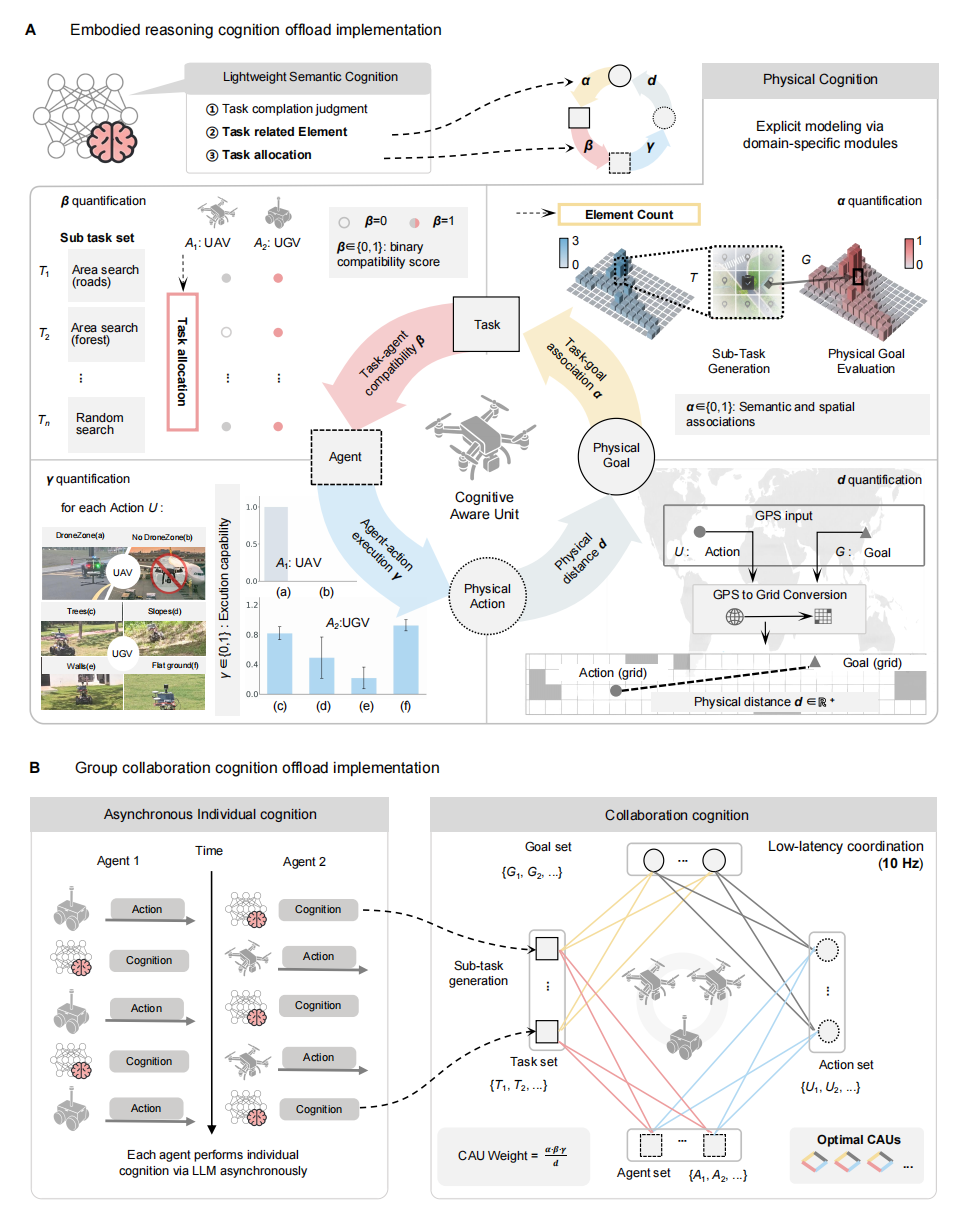
\includegraphics[width=0.88\linewidth,height=0.82\textheight,keepaspectratio]{figures/fig07_cau_custom.png}
\caption{异构多智能体搜索中的认知卸载实现：由CAU承担具身物理推理，由CAU图承担群体协同优化}
\label{fig:report-7}
\end{figure}

\begin{figure}[htbp]
\centering
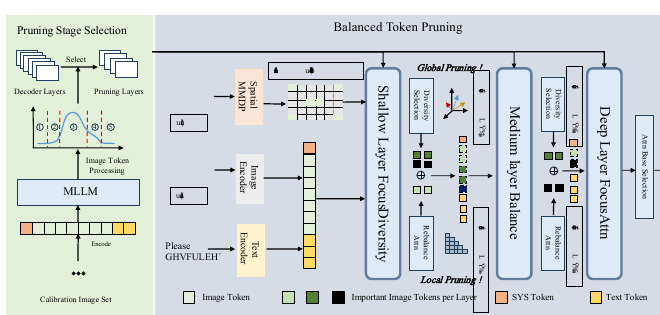
\includegraphics[width=1.00\linewidth,height=0.82\textheight,keepaspectratio]{figures/fig08_btp_framework.png}
\caption{Balanced Token Pruning分阶段视觉词元剪枝框架}
\label{fig:report-8}
\end{figure}

CAU与BTP分别作用于系统外部和模型内部。前者把语言模型之外可验证的物理与协同过程结构化，降低“大模型承担一切认知”的系统负担；后者根据网络深度动态分配视觉计算预算，降低“大量视觉词元在所有层等价计算”的模型负担。二者共同构成“高阶认知集中、物理执行分散、计算资源动态调整”的复杂系统规划机制，也说明认知卸载既可以改变模块职责，也可以改变同一模型内部的信息流。

\subsection*{实验结果与分析}
实验围绕准确性、路径效率、计算开销、推理时延、资源压缩率和真实系统闭环能力展开。由于五项工作分别针对具身视频推理、城市空中导航、自主探索、视觉语言模型加速和异构空地协同搜索，不同任务的指标定义并不一致，因此不对绝对数值进行简单横向排名，而是重点分析每种方法相对于其对应基线的变化，并判断性能改进是否与所提出的认知卸载机制一致。

实验分析同时关注“效果是否提高”和“为什么提高”。如果一个方法仅依赖更大的模型、更强的GPU或更多训练数据获得更好结果，并不能直接证明认知卸载有效。因此，本章优先使用模块消融、输入规模变化、调用时延、路径行为和真实系统执行现象解释改进来源，特别关注关键帧、强化学习、记忆图、近端规划器、区域序列规划器、词元平衡策略和CAU结构分别带来的作用。

\subsubsection*{快慢认知分流的复杂语义理解与按需推理}
Embodied-R在公开具身视频空间推理任务上验证大小模型协作机制。系统使用大规模视觉语言模型将关键帧转换为结构化语义序列，再训练3B规模语言模型执行空间推理。训练数据规模约为5千条具身视频样本，说明该方法并非依靠大规模重新训练视觉基础模型，而是把训练重点集中在较小的推理模块上。最终总体平均准确率达到51.1\%，较OpenAI-o1高13.9个百分点，较Gemini-2.5-Pro高10.3个百分点。

这一结果的意义首先在于证明了“感知能力最强的模型不一定需要直接输出答案”。大规模视觉语言模型已经能够稳定识别对象和场景，但在长视频空间关系推理中，直接端到端回答会同时受到视觉冗余和推理链不稳定的影响。将视觉证据先转化为语义，再交给专门训练的小模型后，任务接口变得更明确，推理器可以把容量集中在跨帧关系组合，而不是重复学习视觉编码。

关键帧实验直接验证了输入卸载的有效性。筛选前平均输入约32帧，筛选后降低至20.7帧，减少约三分之一视觉帧的同时，总体准确率由49.5\%提高到51.1\%。这表明原始视频中存在大量对最终空间推理贡献有限的重复观测，适当去除这些帧不会必然损失信息，反而能够减少无关视觉内容对后续语义和推理的干扰。

效率指标与这一机制一致。采用关键帧后，训练时间由约127.87小时降低到111.70小时，推理时间由约243.68秒降低到157.55秒，后者下降约35\%。时延降低不仅来自帧数减少，也来自最终推理由较小语言模型完成。与单纯缩小视觉模型不同，该框架保留大模型作为冻结感知器，因此效率优化没有以完全放弃开放视觉能力为代价。

协作消融进一步说明性能收益来自“感知—推理分工”，而非某个基础模型本身。在使用相同关键帧和相同视觉语言模型的情况下，协同推理框架的整体准确率约为视觉语言模型直接作答方案的1.5倍。也就是说，同一套视觉感知证据经过结构化中间表示并交由专门推理器处理后，可以产生明显不同的最终效果，这支持了显式认知接口的必要性。

强化学习消融揭示了慢思考能力的来源。去除强化学习后，模型在UrbanVideo-Bench上的性能下降约27.9\%，在VSI-Bench上的性能下降约20.6\%。直接对较小视觉语言模型进行强化学习的结果仍明显低于“强视觉感知器加轻量语言推理器”的分工路径，说明困难并不只是缺少某一种训练算法，而在于需要先把视觉感知和空间推理的任务边界划清。

逻辑一致性奖励也表现出明确作用。训练前，模型的思考过程与最终答案保持逻辑一致的比例约为46.01\%；加入对应奖励后提升至99.43\%。这说明只评价最终答案容易允许模型通过猜测或模式偏置获得奖励，而过程一致性能够迫使模型形成可以支持最终结论的推理链。案例中逐渐出现对象关系分解、系统分析、上下文整合和答案复核等稳定模式，与“慢思考”设计目标一致。

在跨数据集测试中，强化学习得到的推理策略也表现出比监督微调更稳定的迁移能力。其原因在于强化学习并非要求模型复述固定推理模板，而是围绕任务正确性和逻辑一致性优化行为。对于新的视角、对象组合或空间关系，模型仍可以利用相同的分析过程进行组合。这也提示复杂具身任务中，推理过程的结构学习可能比扩大固定格式训练样本更有价值。

\begin{figure}[htbp]
\centering
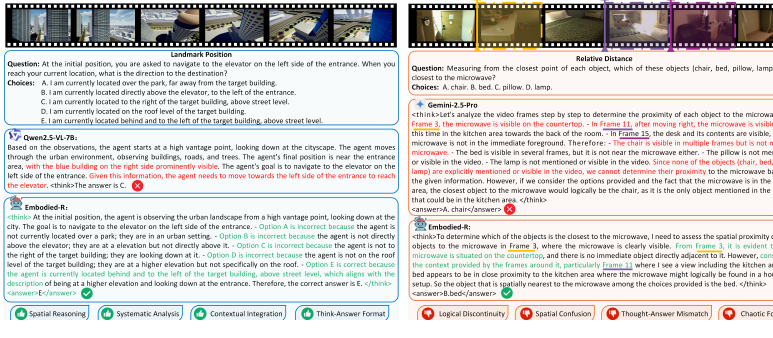
\includegraphics[width=1.00\linewidth,height=0.82\textheight,keepaspectratio]{figures/fig09_embodied_results.png}
\caption{Embodied-R案例与强化学习消融结果：模型形成系统分析和上下文整合的慢思考模式}
\label{fig:report-9}
\end{figure}

训练过程本身进一步揭示了慢思考能力形成的时间结构。准确性奖励在训练早期逐步上升，说明模型并非通过少量步数立即记住答案模式，而是在持续采样和相对比较中逐渐学会更稳定的空间关系组合；格式奖励很快趋近稳定，表明“先思考、后回答”的输出规范较容易建立；逻辑一致性奖励在后续阶段加入后迅速提高，并与准确率保持较高比值，说明模型开始从“给出正确选项”转向“让分析过程真正支持正确选项”。响应长度则从早期较长且波动的状态逐步收敛到更紧凑区间，反映训练没有简单鼓励无限延长思维链，而是形成适合该类空间任务的推理长度。

直接对同规模视觉语言模型进行强化学习的对照还说明，推理训练不能弥补感知上限。视觉语言模型同时承担画面理解和关系推理时，其有限容量需要在两个任务之间分配；而协作框架将高质量感知固定在大模型侧，小模型只需学习如何消费结构化语义，因此同等训练资源能够更集中地改善推理能力。这个结果与前述协作消融共同表明，性能提升来自“强感知基础＋专门推理训练”的组合，而不是单纯把强化学习应用到任意模型即可获得。

分布外测试提供了另一层证据。强化学习模型在EgoSchema和MVBench上的表现相对监督微调更加稳定，尤其在训练数据分布明显变化时仍保持竞争力。其原因可以从推理过程理解：监督微调更容易拟合训练集中固定表述，而奖励优化更强调最终关系判断是否正确、推理与答案是否一致。模型因此更倾向于形成可重复使用的分析步骤，例如先确认运动方向、再更新对象相对位置、最后结合问题进行判断。这些步骤对具体物体类别依赖较弱，更容易迁移到新的视觉内容。

\begin{figure}[htbp]
\centering
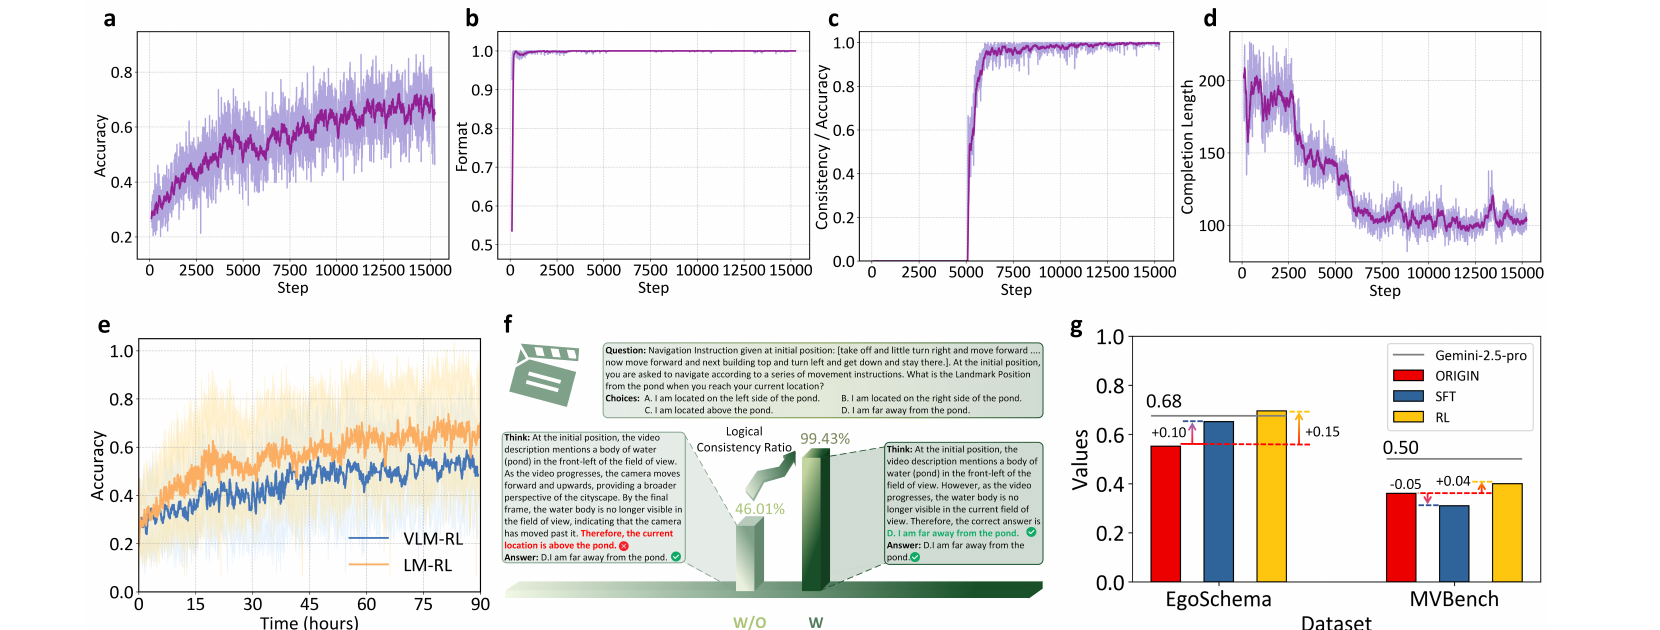
\includegraphics[width=1.00\linewidth,height=0.80\textheight,keepaspectratio]{figures/fig14_embodied_training_dynamics.png}
\caption{强化学习训练动态、逻辑一致性改进及分布外泛化结果}
\label{fig:report-14}
\end{figure}


同时，该方法仍存在明确边界。关键帧筛选若遗漏决定性视角，后续小模型无法从不存在的语义中恢复证据；大型感知模型若错误识别对象或相对关系，小模型可能在错误前提上得到逻辑上自洽但实际错误的结论；当任务需要极强开放世界知识时，3B推理器的知识范围仍可能成为限制。因此，后续系统更适合在接口处加入语义置信度和回退机制，而不是把所有问题永久固定到轻量通道。

总体而言，该组实验验证了三层因果关系：关键帧减少冗余输入，结构化语义把感知与推理解耦，强化学习使轻量模型形成专门化慢思考。准确率提升和时延下降同时出现，说明认知卸载并非单纯以性能换效率，而是在重新分配模型职责后获得更合理的计算—能力匹配。

\subsubsection*{全局—局部空间分解的复杂空间认知与记忆规划}
CityNavAgent在连续城市空中视觉—语言导航任务上验证层次化语义规划和全局记忆。其主要实验包含25个城市级场景，覆盖城区、工厂、公园和村落等不同环境，并包含大量开放类别城市对象。在更细粒度的指令数据中，自然语言被分解为多个具有阶段关系的子指令，使方法能够检验从长语言目标到连续三维航点的层次化映射能力。

在主要对比中，CityNavAgent的成功率达到28.3，SPL达到23.5，导航误差为95.1。作为对照，LM-Nav的成功率为23.6、SPL为19.2、导航误差为119.4。换言之，CityNavAgent不仅更容易最终到达目标，其成功轨迹的路径效率也更高，同时终点与目标之间的残余距离更小。原材料中概括的导航误差降低约20\%与这一量级一致。

层次化规划对结果的贡献可以从连续动作空间理解。城市无人机直接预测远距离最终目标时，语言与空间之间缺少中间锚点；而地标级规划先把指令分成有顺序的阶段目标，物体级规划再从当前可见对象中寻找最有可能通向阶段目标的区域，运动级规划最后产生局部航点。每一层只解决自身尺度的问题，使错误不会一次跨越整个长距离航程。

语义地图消融验证了“开放语义必须落到度量空间”这一点。去除语义地图后，成功率由28.3降至23.6，SPL由23.5降至19.2，导航误差由95.1增加到119.4。仅有语言描述而缺少对象与三维位置之间的明确映射时，高层模型即使正确理解了“应该去哪里”，也更难把结论稳定转换为连续空间中的可执行目标。

全局记忆的作用更加显著。去除记忆图后，成功率下降至11.7，SPL下降至9.1，导航误差上升至206.1。长距离城市环境中，相似道路和建筑容易导致机器人重复进入已经探索过的区域；拓扑记忆保存成功轨迹后，历史可达关系可以直接被图搜索复用，使模型不必在每次遇到熟悉区域时重新依赖当前视觉和长上下文推断。这说明长期空间知识更适合作为外部图结构持续积累。

不同语言模型的消融还反映了高层语义能力的边界。较弱模型在物体级规划中更容易出现幻觉或非结构化输出，导致候选对象不能可靠映射到语义地图；更强语言模型在复杂指令和弱语义关联中表现更稳定。然而，即便更换高层语言模型，语义地图和拓扑记忆仍然承担同样职责，说明系统性能不是完全依赖单一模型规模，而是由语言推理与空间结构共同决定。

案例分析揭示三类典型失效。第一类来自指令本身的歧义，例如多个相似建筑都可能对应同一语言描述；第二类来自开放词汇感知错误，例如反光、远距离小目标或外观相似设施造成误识别；第三类来自物体级语义推理错误，即模型虽然正确识别了场景对象，却错误判断哪一个对象最可能通向不可见地标。这三类错误分别对应语言目标、视觉证据和高层选择，层次化架构使其能够被逐层定位。

\begin{figure}[htbp]
\centering
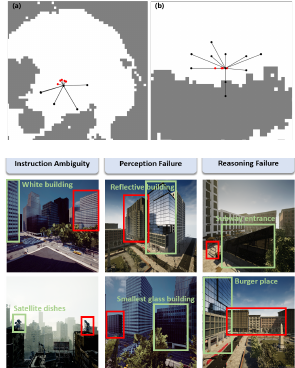
\includegraphics[width=0.52\linewidth,height=0.82\textheight,keepaspectratio]{figures/fig10_city_cases.png}
\caption{CityNavAgent航点预测与典型失败案例：红色为预测或误识别目标，黑色为参考位置}
\label{fig:report-10}
\end{figure}

从不同难度子集进一步观察，方法的优势并非在所有指标上机械一致，而是与长程语义和记忆需求相关。简单任务中，CityNavAgent的成功率和路径效率已经明显高于主要对照，且导航误差显著减小；正常难度下，成功率和SPL继续保持领先，说明三级语义分解能够在指令更长、候选更多时稳定缩小动作搜索空间。在困难子集中，部分对照方法在单一SPL或终点误差上仍可能接近甚至略优，这说明层次化语义规划并不能保证每条成功轨迹都达到最短，但其总体平均成功率、路径效率和误差组合更稳定。该现象也提示，城市导航的评价不能只观察某一个指标，而应同时考虑能否到达、到达路径是否高效以及最终残余误差。

导航过程的逐步可视化进一步说明了记忆与常识推理如何参与实际决策。对照方法在遇到不可直接观察的下一地标时容易继续沿当前方向探索，或者在视觉相似的街区中逐渐偏离；CityNavAgent则先从当前场景识别可见对象，再利用常识判断哪些对象与下一地标具有语义联系。当系统到达已记录的记忆节点后，可以直接在历史图中检索后续路径，而不再重复执行开放探索。由此，视觉感知、语义关联和记忆检索并不是并列模块，而是在不同导航阶段接替主导作用。

\begin{figure}[htbp]
\centering
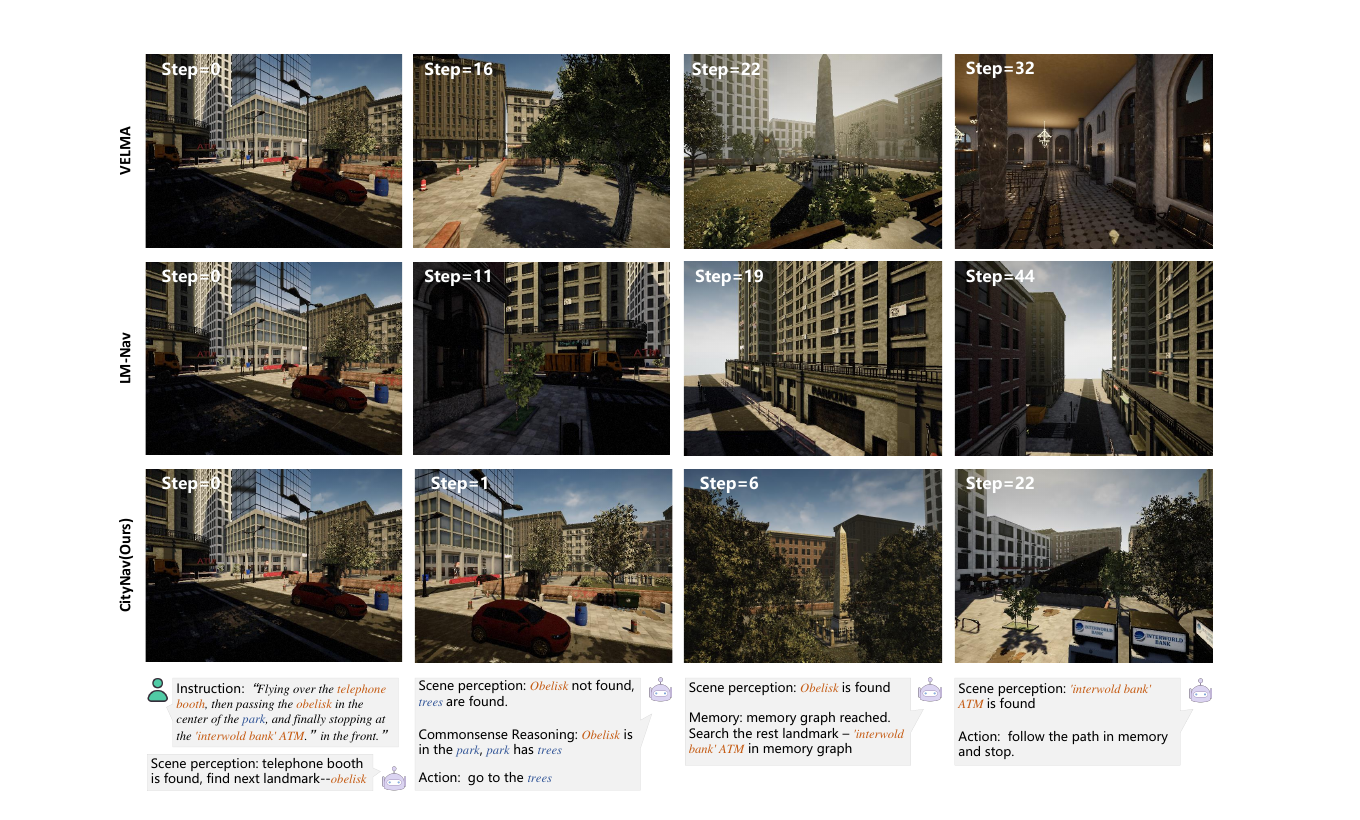
\includegraphics[width=0.96\linewidth,height=0.80\textheight,keepaspectratio]{figures/fig15_city_navigation_process.png}
\caption{不同导航方法的连续执行过程及层次化语义推理与记忆复用示例}
\label{fig:report-15}
\end{figure}


SCOPE则在多类仿真环境和真实无人机平台上验证骨架图与按需规划。仿真比较覆盖复杂办公区、迷宫、隧道和多层办公环境，并同时记录探索完成时间、单周期规划计算量、飞行速度、路径长度和覆盖体积。与只看“找到多少未知空间”相比，这组指标能够更完整地反映一个探索算法是否适合边缘无人机长期运行。

综合多个场景，SCOPE的平均规划计算开销相比现有方法降低约86.9\%。在复杂办公环境中，其探索时间约158.24秒，单次平均计算开销约7.71 ms，路径长度约297.92 m，覆盖体积约1727.61~m$^3$。这表明低频全局规划并没有使机器人失去主要覆盖能力，反而通过局部高频规划维持了较平滑的探索推进。

与FALCON等方法比较时，SCOPE在复杂办公环境中的探索时间可缩短约7.98\%，同时其计算负担显著更低。不同场景中路径长度并不始终最短，例如在部分多层环境中，引入层次规划可能产生约6\%的额外路径，但对应计算负载可降低约93.2\%。这揭示了方法的真实工程取舍：它不追求每个场景的绝对全局最短路径，而优先保证低计算开销、轨迹连续性和可实时更新。

消融实验进一步区分近端规划和区域序列规划的作用。去除近端规划器后，探索时间增加约14.5\%，计算开销增加约303.2\%，因为系统不得不更加频繁地调用全局规划。去除区域序列规划器后，虽然节省了一部分计算，但整体探索效率下降约17.7\%，说明纯局部策略容易在区域之间缺乏战略顺序。两者组合恰好体现“局部高频、全局低频”的职责互补。

骨架表示本身也对效率具有决定作用。若将紧凑增量骨架替换为更传统的Voronoi类结构，计算开销可显著增加，而探索收益并不成比例。SCOPE的骨架维护占总规划计算的一部分，但单次维护仍保持毫秒级；核心近端规划更轻量，而区域序列规划虽然单次开销较高，却只在需要跨区域决策时偶尔触发。总体平均成本因此能够保持在边缘平台可接受范围。

真实平台实验验证了这一结构不依赖高端桌面GPU。系统可部署于Jetson Orin NX等机载计算平台，结合深度相机、视觉惯性定位和飞控进行在线探索。在实验室与杂乱办公场景中，平均规划开销保持约5.8--5.9 ms量级，并完成数百立方米空间覆盖。真实实验说明“减少全局规划调用”不仅是仿真中的时间统计，也能够转化为机载系统的实时余量。



不同环境中的单周期计算分布进一步验证了SCOPE的效率优势并非来自某一个特定场景。无论在经典办公区、复杂办公区、迷宫还是隧道环境中，所提出方法的每次规划计算时间都整体位于更低区间，而且波动范围相对受控。相比需要频繁执行全局前沿分解或全局目标优化的方法，其计算量对前沿数量和地图复杂度的敏感性更低。特别是在复杂办公和迷宫场景中，基线方法的计算分布明显向高时延区域扩展，而分层规划仍保持较低中位数，说明局部高频与全局低频的结构能够抑制地图规模增长带来的在线负担。

这一结果与消融表中的模块时间分布相互印证。骨架维护虽然占据单周期计算的较大比例，但其绝对时间仍处于毫秒级；近端规划器本身更加轻量，而区域序列规划的单次成本较高，却通过低频触发被摊薄。因而总平均时间并不是由最慢模块决定，而由“每个模块一次运行多快”和“它在整个任务中多久运行一次”共同决定。该结论对于认知卸载尤其重要，因为高成本模块只要从固定周期调用转变为条件触发，即使单次计算不变，也可以显著降低长期平均负担。

\begin{figure}[htbp]
\centering
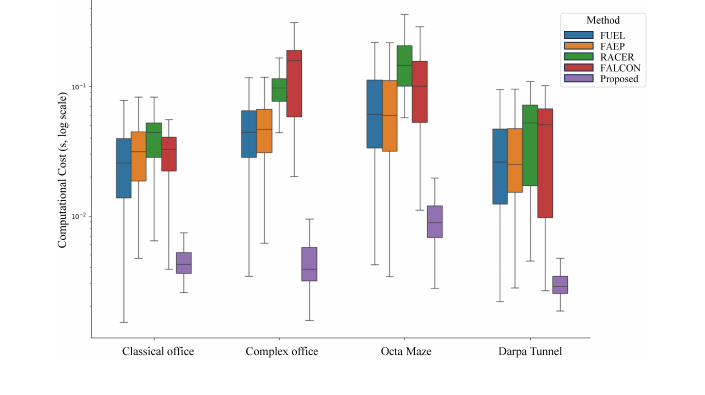
\includegraphics[width=0.78\linewidth,height=0.70\textheight,keepaspectratio]{figures/fig16_scope_computation_boxplot.png}
\caption{不同探索环境下单次规划计算时间分布对比}
\label{fig:report-16}
\end{figure}

\begin{figure}[htbp]
\centering
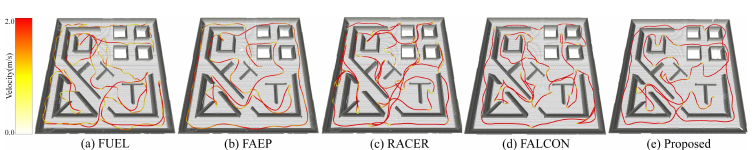
\includegraphics[width=1.00\linewidth,height=0.82\textheight,keepaspectratio]{figures/fig11_scope_results.png}
\caption{SCOPE多环境探索结果与复杂办公场景轨迹对比}
\label{fig:report-11}
\end{figure}

综合CityNavAgent与SCOPE可见，全局—局部空间分解在两种不同任务中呈现出一致机制。语言导航通过语义层级和拓扑记忆压缩长时程目标及历史状态，自主探索通过骨架和隐式区域压缩大规模未知空间；两者都让全局模块承担低频方向选择，让局部模块承担高频连续动作。实验中的成功率、路径效率和毫秒级规划开销共同表明，大空间任务并不需要在每一个周期都执行完整全局推理。

这类方法仍存在边界。CityNavAgent的实验主要建立在连续城市仿真环境中，真实飞行中的通信、控制误差和动态障碍尚需进一步验证；SCOPE的隐式区域依赖当前地图与几何探针，当环境快速变化或大范围户外感知稀疏时，区域估计可能过期。因此，后续可在全局层加入置信度、地图时效性和动态触发条件，使“何时重新进行全局认知”本身也成为可学习或可适应的变量。

\subsubsection*{高阶认知—灵敏执行协同的复杂系统规划}
Balanced Token Pruning首先从模型内部验证视觉计算卸载。视觉语言模型中并非所有图像词元在全部网络层都同等重要。实验跨多种视觉语言模型和基准任务进行，在平均裁减约78\%视觉词元的情况下，仍可保留原模型约96.7\%的平均性能。这说明大量视觉计算存在结构性冗余，关键不在于“是否可以剪”，而在于“在哪一层、依据什么标准剪”。

在LLaVA-1.5-7B上，原始视觉输入包含576个词元。当词元压缩至128个时，BTP仍可保持约98\%的原模型性能。相比只依据当前层注意力的策略，平衡方法在后续深层表示上更稳定；相比只追求多样性的策略，其当前问题相关输出又具有更好保持。这与方法提出的局部—全局双目标一致：注意力保证当前层相关性，多样性避免删除后续仍可能需要的视觉信息。

真实时延结果也说明剪枝算法本身必须足够轻。以同一模型为例，未剪枝单步相关计算约为0.145秒，BTP在128词元配置下约为0.134秒，在64词元配置下约为0.120秒。某些需要复杂两两多样性计算的方法虽然理论上减少了后续词元，却可能因选择开销使端到端时间反而增加。BTP通过空间初始化降低多样性筛选成本，使理论计算量下降能够真正转化为运行时间收益。

资源占用同样得到降低。在部分LLaVA配置中，视觉相关键值缓存可从约0.34 GB降低到约0.11 GB；对于使用更多高分辨率视觉词元的模型，缓存下降幅度更为明显。这对于机器人边缘部署尤其重要，因为显存不仅要容纳语言模型，还要同时服务感知、地图、规划和控制线程。视觉词元压缩释放出的资源可以用于更高分辨率输入、更长文本上下文或其他实时模块。

校准层选择和分阶段权重的消融进一步表明，均匀地在任意层删除相同数量词元并非最优。浅层信息会影响更多后续层，因此应更重视代表性和多样性；深层距离最终输出更近，可以更强调当前文本问题的注意力相关性。通过少量校准样本确定剪枝阶段后，不需要针对每个下游任务重新训练主体模型，提升了方法迁移到不同视觉语言模型的可用性。

\begin{figure}[htbp]
\centering
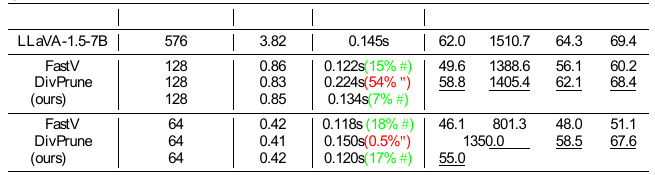
\includegraphics[width=1.00\linewidth,height=0.82\textheight,keepaspectratio]{figures/fig12_btp_results.png}
\caption{Balanced Token Pruning在不同压缩率下的性能与实际推理时间对比}
\label{fig:report-12}
\end{figure}

CAU方法则从系统外部验证认知过程卸载。实验首先分析端到端大模型在异构搜索任务中的不同能力。语义相关的识别和判断通常保持较高水平，但涉及具身物理和上下文组合时性能明显下降。例如，部分物理感知子任务可达到80\%--90\%以上，而上下文推理整体仅约21.5\%；当多个物理条件必须同时满足并最终产生有效动作时，端到端系统整体成功率可下降到约0.9\%。这说明单个子问题“看起来都能回答”并不意味着完整动作链能够可靠闭环。

CAU将物理认知卸载后，高层大模型只完成任务状态、要素相关性和平台推荐等语义判断，整体语义认知准确率达到约94.3\%。其中任务完成判断约99.1\%，要素相关性约95.1\%，后者接近人工判断水平。由于动作可行性由地图、平台能力和几何约束验证，语言模型不再需要通过自由生成承担“是否会碰撞”“是否能通过”“是否违反禁飞”等确定性问题。

输入规模的变化非常显著。相对于端到端方案，结构化认知卸载可减少约97.7\%的大模型输入词元，同时总体任务级认知准确性提高约93.4个百分点。两者同时发生说明系统不是通过给大模型更多上下文获得性能，而是通过删除原本不应由语言模型处理的物理信息，让输入只保留真正需要语义理解的部分。更短上下文还直接降低首词元等待和生成延迟。

异步执行进一步改善多智能体等待时间。在端到端同步方案中，无人机平均可能等待约17.29秒以完成一轮集中式推理与同步；采用认知卸载和异步规划后，等待时间可降低到约0.04秒量级。总体规划时延相对端到端基线降低99\%以上，实验进一步报告可达到约99.9\%的量级。这里的收益不仅来自单次优化器求解快，更来自系统关键路径被重新设计：不同智能体不再为一次全局语言推理互相阻塞。

真实系统由3架微型无人机和1辆无人车组成。无人机具有较大的俯视搜索范围，适合快速发现道路、目标或大尺度场景关系；无人车具有近地移动和细粒度接近能力，能够处理更贴近地面的任务。系统通过无线通信连接中心规划节点，CAU图持续维护候选行为并进行任务分配，使两类平台根据自身能力承担不同搜索阶段。

在约88 m乘64 m的真实方形区域中，系统在无先验目标地图条件下执行自然语言搜索，并在约159秒总时间内完成目标定位，其中包含初始化时间；在约44 m乘32 m的十字路口场景中，系统同样能够根据自然语言要求协调空地平台完成行人搜索。多次真实测试中，环境要素识别准确率保持约95.3\%，表明高层语义变量能够在真实感知噪声下保持较高稳定性。

真实结果还体现了CAU图的可解释性。无人机观察到具有任务相关性的候选区域后，并不是直接让大模型输出“让某机器人去那里”，而是先把区域映射为目标节点，再结合平台能力、动作可执行性和距离生成候选单元。若某个候选违反禁飞、地面障碍或平台任务类型约束，会在进入最终分配前被拒绝。最终分配因此能够追溯到明确的语义、能力和物理证据。

从规模扩展角度看，CAU图的候选组合在理论上仍随智能体、动作、目标和任务数量增加，但大量不兼容和不可行动作可以通过结构化约束提前剪枝。实际常见规模下规划保持百毫秒以内，并可按约10 Hz更新。与把所有原始图像和历史动作重新送入大模型相比，其计算增长主要与当前有效候选关系相关，而不是直接与全部历史词元长度绑定。

\begin{figure}[htbp]
\centering
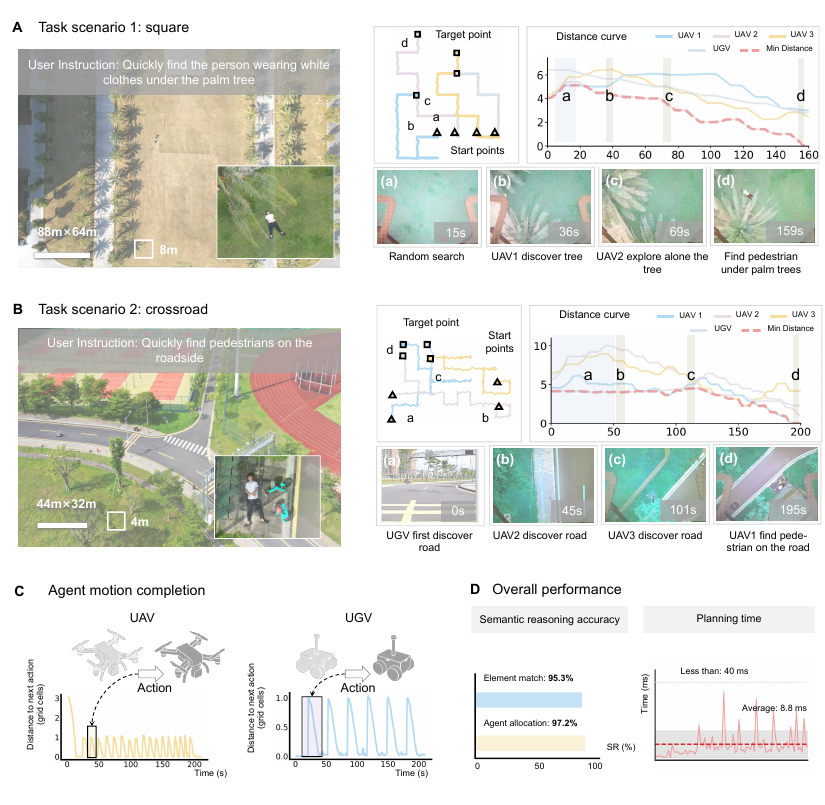
\includegraphics[width=0.96\linewidth,height=0.82\textheight,keepaspectratio]{figures/fig13_cau_results.png}
\caption{CAU异构空地系统真实场景验证及总体性能}
\label{fig:report-13}
\end{figure}

从BTP的结果还可以看到，压缩率与收益并不是线性关系。随着视觉词元减少，后续层的注意力和缓存开销持续下降，但当保留数量过低时，关键视觉证据被删除的风险会迅速增加。因此，128词元附近能够在部分模型上保持接近完整性能，而进一步压缩到64词元虽然获得更明显的时延下降，却需要接受更大的任务性能波动。分阶段平衡策略的价值就在于把性能下降推迟到更高压缩区间，使系统可以根据实时资源选择不同工作点，而不是只有“完整模型”和“极端压缩”两种状态。

实际运行时间也表明，剪枝方法必须把选择开销纳入总成本。若某种算法为了判断词元重要性需要复杂的两两比较，即使后续注意力计算减少，前置筛选本身也可能抵消收益。BTP的空间初始化利用图像词元原有布局降低选择复杂度，因此在不同保留数量下能够看到更稳定的端到端加速。这种结果说明，模型级认知卸载不能只报告理论FLOPs，还应把剪枝算法本身、缓存访问和实际硬件执行时间共同计入。

CAU的仿真实验则展示了任务完成过程随时间的差异。对于大尺度、小尺度和异构配置，多种基线在最近智能体到目标的距离曲线上往往出现较慢下降或长时间停滞，而结构化方法能够更快将有效智能体分配到具有任务价值的目标区域。不同任务中的总完成时间、平均路径长度、重复访问和成功率并不完全同步，但整体趋势表明，只要高层语义相关性与物理可行性被分开处理，系统就更容易避免“语义上合理但执行无效”的动作消耗。

更值得关注的是失败模式的变化。端到端方案中的失败通常发生在完整动作链末端，很难判断是语义、物理还是协同哪个环节导致；CAU中，很多不可行动作在候选生成阶段已经被拒绝，因此进入真实执行的错误更集中在语义误判或未建模约束。也就是说，认知卸载不仅提高最终成功率，还把错误从“不可解释的端到端失败”转化为“能够定位到具体约束或语义变量的局部失败”。这种错误结构变化对于后续系统调试和安全验证具有直接价值。

从规模增长趋势看，结构化候选数量仍会随着机器人和目标增加，但增长发生在经过能力与可行性筛选之后。无效组合被提前删除，使求解器实际面对的图规模远小于理论笛卡尔积。与此同时，各智能体采用异步执行，群体规模增加并不会自动要求所有主体在同一时刻重新调用大模型。因而系统扩展性来自两方面：空间上减少无效候选，时间上减少同步等待。二者共同解释了规划延迟在多主体实验中仍能够维持较低水平。


CAU实验也说明认知卸载并非否定大模型。高层语义判断仍是整个系统理解开放自然语言任务的入口，尤其是任务要素与场景对象之间存在非固定语义关系时，纯规则难以覆盖。方法真正改变的是大模型输出的粒度：它不再直接产生一条不可检查的完整动作链，而只更新结构化语义变量，随后由确定性模块把语义转化为物理可执行行为。大模型从“系统控制器”转变为“高阶认知服务”。

与此同时，现有真实验证仍主要集中在3架无人机与1辆无人车、相对稳定通信和静态或低动态目标场景。更大规模群体、快速动态障碍、通信间歇和任务持续变化会对CAU图更新、目标时效性和局部自治提出更高要求。因此，后续需要在保持结构化可验证性的同时，引入分布式候选维护、动态目标预测以及通信失效下的本地回退机制。



从训练资源角度进一步看，Embodied-R的结果说明“将学习预算投入哪一部分”与“总模型规模”同样重要。大型VLM主要承担已经具备较强能力的视觉感知，保持冻结可以避免昂贵的多模态强化学习；训练集中约5千级样本则用于激活3B语言模型的空间推理能力。该安排把有限训练资源集中在真正的能力短板上。实验中直接强化学习同规模VLM的上限低于协作框架，也说明如果基础感知本身不足，强化学习很难仅靠奖励把缺失视觉能力补出来。

三阶段训练曲线还能够解释为什么逻辑一致性奖励需要后置。训练初期模型尚未稳定遵循输出格式，此时直接强调思维链质量会使奖励稀疏且噪声较大；当格式与答案能力逐渐形成后，再要求推理与结论一致，模型才有稳定基础进行过程优化。最终逻辑一致性由约46.01\%提升到99.43\%，说明后期奖励并非只是润色文本，而是显著改变了“正确答案是否具有正确理由”这一内部行为特征。

分布外结果进一步提供了对训练方式的比较。监督微调容易学习训练集中常见的回答形式和语义模式，在场景分布变化后可能出现迁移不稳定；强化学习则围绕任务结果和过程一致性选择策略，使模型有机会形成更通用的分析步骤。对于具身空间任务，这类步骤包括确认自身动作、更新对象相对关系、识别新增证据、再根据问题进行组合。它们与具体对象类别关系较弱，因此更容易迁移到不同室内外场景。

CityNavAgent的消融结果可以进一步从误差累积角度理解。没有语义地图时，每次高层推理与物理位置之间都缺少稳定映射，单步航点偏差会逐渐累积；没有记忆图时，机器人即使此前已经成功经过某一区域，也无法利用历史路径快速恢复，容易重新进入探索状态。两种模块的作用不同：语义地图提高“当前一步往哪里走”的正确性，记忆图提高“长期运行是否反复走错或遗忘”的稳定性。因此，记忆消融造成的长程性能下降更明显。

对不同LLM的比较也表明，结构化外部表示并不能完全消除语言模型能力差异。较弱模型在OROI推理中仍可能产生幻觉或不符合格式的输出，更强模型对弱语义联系处理更稳定。但由于候选必须落到已检测对象和三维语义地图中，即使模型能力不同，其错误范围也受到接口限制。这说明认知卸载并不是让模型质量变得无关，而是减少模型错误可以影响系统的自由度。

SCOPE的消融则提供了调用频率与计算负担之间的直接证据。去掉近端规划器后，全局规划不得不更频繁介入，平均计算显著增加；去掉区域序列规划器后，单步计算可能降低，但机器人缺少跨区域战略，整体探索效率下降。真正有效的不是“只用局部”或“只用全局”，而是根据局部目标是否耗尽决定何时切换。该实验支持把触发条件视为算法组成部分，而不是简单的工程调参。

SCOPE在部分场景中接受轻微路径增长却获得大幅计算下降，也揭示了机器人系统评价中容易忽略的一点：全局最短路径并不是唯一目标。机载计算资源还要同时运行定位、建图、避障、通信和感知，规划线程长期占用过多资源可能影响整个系统稳定性。若增加少量航程能够换取数量级更低的规划负担，并减少轨迹振荡，对资源受限平台往往是更合理的总体最优。

真实平台毫秒级规划结果尤其重要，因为仿真中的算法速度并不一定能转化到机载部署。地图更新、传感噪声和实际控制都会增加计算与状态不确定性。SCOPE在真实环境中仍保持低毫秒级平均规划开销，说明增量骨架、近端规划和低频区域序列并非依赖理想仿真条件。该结果也为认知卸载提供工程证据：被外化的拓扑结构确实能够在有限边缘算力上持续维护。

BTP的实验则表明理论压缩率必须与真实运行时间联合分析。一个方法即使减少更多视觉词元，如果选择这些词元需要复杂矩阵运算，整体时延可能并不下降。BTP通过空间初始化和分阶段选择控制附加开销，因此在较高压缩率下仍能够获得实际加速。对于机器人应用，端到端延迟比理论FLOPs更关键，因为控制系统只能利用真实释放出来的时间预算，而不能利用纸面计算量下降。

在不同视觉语言模型上保持较稳定收益还说明，BTP利用的是视觉词元冗余和网络层次的普遍结构，而不是某一个模型中特定的权重模式。不同模型的图像词元数量、视觉编码器和语言骨干可以不同，但“浅层删除影响更多后续层、深层更接近当前输出”的基本关系保持一致。因此，通过小校准集确定阶段后，方法能够以较低改造成本迁移，为模型级认知卸载提供了较强通用性。

CAU实验最关键的现象是端到端系统在单项能力与完整闭环之间存在巨大落差。某些物理感知或语义判断单独测试时并非完全失效，但当任务要求连续完成场景理解、上下文推理、动作可行性判断并最终给出有效行为时，错误会逐级相乘，使任务级成功率降到很低。CAU把其中可验证的物理过程拆出后，大模型只保留语义判断，整体准确性大幅恢复。这说明复杂系统中的主要问题往往不是某一步完全不会，而是多个概率步骤串联后的误差累积。

输入词元减少约97.7\%与准确率提升同时出现，更能说明“上下文越多越好”并不成立。端到端提示词中大量物理状态虽然看似为模型提供更多信息，却要求模型自行理解坐标、距离、可达性和平台差异，增加了认知负担。结构化模块直接消费这些数据后，大模型看到的信息更少但更聚焦，语义判断反而更稳定。这与Embodied-R删除重复视觉帧后准确率不降反升形成呼应：关键是有效信息比例，而非绝对输入量。

从时序结果看，异步机制带来的收益也不能简单归因于求解器更快。端到端同步框架中，一轮联合推理包含机器人运动完成、状态收集和语言生成等多个串行步骤，最快机器人会被最慢机器人拖住；CAU框架中，语义更新、图求解和运动并行推进，机器人等待时间接近局部规划时间。系统级99\%以上时延下降因此来自架构关键路径变化，而不仅是把某个函数优化了若干毫秒。

真实方形区域和十字路口实验进一步验证了结构化任务分配的行为合理性。空中平台凭借视野优势更适合快速获得大尺度目标线索，地面平台则能够完成近地接近与局部搜索。CAU图不需要在提示词中写出固定的“先无人机后无人车”规则，而是根据任务语义、目标位置、平台能力和距离动态计算候选。不同场景下形成的分工因此具有任务依赖性，而不是预设脚本。

从可解释性角度，CAU实验中的约束拒绝同样具有价值。一个候选被舍弃时，可以知道是任务不匹配、平台能力不足、动作不可行还是代价过高；最终被选择的行为也具有明确权重来源。相比端到端模型只输出一个动作文本，这种结构允许研究者统计不同错误类型和拒绝比例，进一步判断系统瓶颈来自语义、地图还是执行约束。可解释性由此成为可以量化的系统属性，而不是仅依赖语言模型生成解释。

综合五项实验还可以观察到一个共同规律：认知卸载收益通常在任务规模扩大或运行时间变长时更加重要。短视频中全部帧尚可一次处理，小地图中频繁全局规划也许仍能运行，少量机器人时同步等待问题不突出，低分辨率图像中词元冗余也较小；但当帧数、空间范围、智能体数量和视觉分辨率增长时，这些成本都会非线性放大。因此，认知卸载不仅是当前算力受限条件下的加速技巧，也是面向更大规模系统保持可扩展性的结构准备。

从实验方法论上，未来还可以在统一平台中同时记录五类指标：高层模型调用次数、单次输入输出词元、外部结构大小、局部与全局规划时间、最终任务性能。这样可以进一步分析不同卸载策略之间的耦合，例如关键帧减少是否同时降低BTP所需视觉词元，拓扑记忆是否减少大模型重新解释历史的次数，CAU任务重分配是否因更高质量空间记忆而减少。当前五项工作分别验证了这些机制，下一步可以把它们置于同一长时程多机器人平台中研究联合收益。



从跨模块误差传播角度看，五组实验还形成了一条较清晰的共同证据链。Embodied-R表明，如果前端保留的是高价值关键帧并将变化显式描述，后端推理模型面对的噪声会减少；CityNavAgent表明，如果语言目标能够落到三维语义位置并由记忆图保存历史可达关系，长时程误差不会完全依赖上下文累积；SCOPE进一步说明，如果全局结构只在必要时更新，局部地图的小变化不会持续放大为全局规划抖动；CAU则通过物理约束过滤阻断语义误差直接传到底层动作；BTP在模型内部利用分阶段剪枝减少冗余，同时尽量避免浅层误删对后续表示产生持续影响。五种机制分别在输入、状态、规划、动作和网络内部建立误差隔离层，使系统不再依赖单一模型一次性保持所有环节正确。

这种结果还说明，复杂系统的效率提升不能简单等价为“每个模块都更快”。有些模块甚至可以保持原有计算复杂度，只要它们的调用时机和输入规模发生变化，长期平均负担就会显著下降。例如区域序列规划器仍然是相对高成本的全局过程，但低频触发使其平均开销可控；大规模视觉语言模型本身并没有被替换，但关键帧、结构化语义和词元剪枝减少了进入模型的信息量与重复计算；大模型在CAU中仍然执行开放语义判断，但不再承担每个控制周期的物理推理。由此，实验评价应同时观察单次时延、调用频率、输入规模和最终任务性能，才能完整反映认知卸载对真实系统的贡献。

因此，后续在统一平台上的联合验证应优先记录这些跨层指标，以判断不同卸载机制能否形成稳定叠加收益，而不是仅比较单一模块的离线性能。

\subsubsection*{综合指标与机制对应关系}
三类创新方向的实验结果虽然来自不同任务，但可以按照“信息卸载、状态卸载、物理过程卸载和计算卸载”建立统一解释。Embodied-R首先减少连续视频中的重复帧，再把视觉内容转化为增量语义；CityNavAgent把长期空间状态外化为拓扑记忆；SCOPE把完整未知空间压缩为骨架和隐式区域；CAU把物理推理和群体协调外化为结构化单元与图优化；BTP则进一步删除模型内部不必要的视觉词元计算。

在准确性维度，认知卸载的作用不是简单减少信息，而是提高“有效信息占比”。关键帧筛选后输入减少但准确率反而提高，说明重复帧并非有效证据；语义地图与记忆图消融导致导航性能明显下降，说明结构化空间信息比单纯扩大语言历史更重要；CAU使任务级认知从接近失效的端到端动作链提升到较高语义准确率，说明将物理约束从语言推理中剥离能够减少错误级联。

在时延维度，五项工作分别缩短了不同关键路径。Embodied-R减少视觉输入并使用轻量推理器；SCOPE减少高成本全局序列规划的调用频率；CAU消除多智能体之间的同步等待；BTP降低单次视觉语言模型内部的词元计算。这些机制可以叠加，因为它们针对的是不同层次的时间消耗，而不是互相排斥的替代方案。

在资源维度，关键帧和BTP分别从“帧级”和“词元级”压缩视觉输入，拓扑记忆和骨架图从“状态表示级”压缩长期空间信息，CAU从“任务描述级”压缩需要送入大模型的上下文。由此可见，复杂系统的资源优化不能只看参数量。即使模型参数保持不变，通过减少输入、缩短上下文、减少调用频率和降低并发等待，也能够显著改变真实部署成本。

在可验证性维度，每种方法都产生了能够被人工或算法检查的中间结果。Embodied-R可以检查关键帧和语义变化，CityNavAgent可以检查地标序列、语义点云和记忆路径，SCOPE可以检查骨架连通与未知区域，CAU可以检查任务兼容、动作可行和最终分配，BTP可以检查不同阶段的词元保留比例。中间表示使系统失败后能够回答“哪一步错了”，而不仅是观察最终成功或失败。

在实时性与最优性的权衡上，多项实验也表现出一致趋势。SCOPE允许部分场景路径略长，以换取大幅计算下降和更平滑飞行；BTP允许在高压缩率下保留略低于完整模型的性能，以换取显存和时延收益；轻量推理器在适用任务范围内承担更多工作，而在开放语义不足时仍可回退大模型。这说明认知卸载不是无条件追求某个单一最优指标，而是根据任务闭环需求重新配置资源。

因此，本章所提出的总体机制可以概括为：让高成本、高泛化能力的模型处理低频但语义复杂的问题，让低成本、结构明确的模块处理高频且可验证的问题；让全局结构提供方向和长期记忆，让局部模块提供连续快速反应；让模型内部有限计算集中到真正重要的视觉信息。实验中准确性、效率和可解释性同时改善，支持了这一能力边界划分的合理性。

\subsection*{讨论与总结}
本章提出的多层次推理方法以认知卸载为主线，把复杂城市场景中的语义、空间和协同认知过程分解为不同层级。快慢认知分流解决“所有视觉问题都直接调用大型多模态模型”的资源失配；全局—局部空间分解解决长时程任务中历史信息难复用和高频全局规划开销过高的问题；高阶认知—灵敏执行协同则解决大模型物理推理不可靠、异构主体同步等待以及视觉计算冗余问题。

从方法层面看，认知卸载首先是一种职责划分原则，而不是某个固定模块。Embodied-R中的卸载对象是连续视觉冗余和最终空间推理，CityNavAgent中的卸载对象是长时程空间记忆，SCOPE中的卸载对象是完整未知空间和周期性全局优化，CAU中的卸载对象是物理可行性与群体组合决策，BTP中的卸载对象则是模型内部冗余视觉计算。不同任务的具体实现不同，但都要求被卸载过程具有明确输入输出和可验证条件。

这一原则进一步给出了大模型在复杂机器人系统中的合理定位。基础大模型最有价值的部分是开放词汇、语言歧义处理、跨模态关联和非封闭知识，而不是替代几何、地图、优化和控制。只要某个问题可以稳定表达为距离、碰撞、图连通、能力匹配或约束优化，就应该优先使用对应结构化工具；只有当结构化工具无法直接决定语义含义时，再调用大模型。这样既不会削弱大模型优势，也能够减少其在非优势领域产生的概率性错误。

从信息流角度看，系统需要建立比“自然语言文本”更丰富的中间接口。语义序列适合表达跨帧变化，三维语义点云适合连接语言对象与度量位置，拓扑图适合长期保存可达关系，骨架图适合表达自由空间主干，CAU适合表达任务—平台—动作—目标之间的物理行为关系。不同接口对应不同认知过程，避免所有模块都通过长文本互相通信。

从调用频率角度看，高层能力不应等同于高频调用。CityNavAgent只在需要阶段目标时利用高层语义，SCOPE只在局部目标不足时启动区域序列规划，CAU只在语义变量变化时需要大模型更新。高频循环由局部几何和结构化算法承担后，系统的控制周期不再与大模型生成时间直接绑定。这是认知卸载能够从离线算法走向真实机器人闭环的关键条件。

从方法边界看，认知卸载并不等同于用固定规则替代学习模型。外部模块的有效性取决于其表示是否覆盖任务关键约束。关键帧若遗漏决定性动作，轻量推理器无法恢复证据；语义地图若包含误检，全局规划可能沿错误地标推进；骨架图若在快速变化环境中更新不及时，会形成过期空间先验；CAU若未编码关键动力学约束，也可能输出形式可验但实际不可执行的计划；词元剪枝若过早删除关键区域，则后续网络层无法重新生成已经丢失的视觉信息。

因此，下一阶段需要把“不确定性”和“回退”纳入认知卸载框架。对于低置信度视觉语义，可以保留多个候选并触发补充观测；对于轻量推理器无法稳定回答的问题，可以回退到更强模型；对于局部规划连续失败，可以提升到全局层重新分解任务；对于任务分配冲突，可以重新计算CAU图并限制大模型只修改相关语义变量；对于词元剪枝，可以依据任务类型、层间表示变化和剩余计算预算动态调整压缩率。

另一个值得强调的方向是长期运行中的知识时效性。拓扑记忆、骨架图和任务图都属于外部长期表示，但真实城市环境并非静态。道路可能暂时封闭，障碍可能移动，目标可能改变位置，通信状态也会变化。因此，未来系统不仅需要“记住什么”，还需要判断“什么时候旧记忆失效”。可以为图节点和边增加时间戳、置信度和更新次数，使历史知识在被复用前重新接受局部观测验证。

在多智能体扩展方面，结构化图优化为规模增长提供了比端到端语言协商更清晰的路径，但大规模群体仍会带来候选组合增加和通信负担。后续可以利用任务区域分区、局部子图和分布式协商进一步限制每个机器人需要处理的候选范围，使中心高层只维护跨区域或跨能力的关键冲突。这样可以延续“高阶低频、局部高频”的原则，从单中心异步架构进一步扩展到分层分布式架构。

在工程部署中，还应建立统一运行监测指标，包括大模型触发率、平均输入词元数、关键帧保留率、语义候选数量、全局规划触发率、单周期规划时延、任务重分配次数、物理约束拒绝率、词元压缩率和任务完成率。只有同步记录这些指标，才能判断性能提升究竟来自认知过程优化、模型规模变化还是硬件差异，并为不同城市应用选择合适的资源预算。


从统一系统视角看，这些监测量还可以进一步构成“认知预算”。传统机器人系统通常只分配CPU、GPU、显存和通信带宽，而在大模型参与闭环后，还需要显式管理高层推理次数、视觉输入规模、历史上下文长度以及全局重规划频率。不同任务阶段可以使用不同预算：环境稳定、目标明确时降低大模型触发率并提高局部自治；观测出现冲突、任务发生变化或局部规划连续失败时，再临时提高高层认知预算。这样，计算资源分配能够随任务不确定性变化，而不是始终按照最坏情况配置。

认知预算还可以与系统安全性建立联系。对于能够由确定性模块验证的动作，高层模型可以只提供候选而不直接控制执行；对于无法完全验证的开放语义判断，则可以要求更高置信度、更多候选或附加观测后再下发。换言之，卸载并不是简单地把“难问题给大模型、简单问题给小模型”，而是根据错误后果和验证能力安排不同的决策权限。越接近物理执行层，越需要明确的约束和可检查条件；越接近任务意图层，越可以保留模型的开放生成能力。

从训练与部署关系看，该框架也减少了“所有模块必须联合重训”的依赖。Embodied-R可以冻结强视觉感知器而主要训练轻量推理器；BTP不改变原视觉语言模型主体参数，通过校准和推理期选择实现压缩；CityNavAgent、SCOPE和CAU中的地图、图结构与优化器均可以独立替换或升级。这意味着系统可以在不推翻整体架构的情况下迭代某一个认知过程。例如，更换新的开放词汇感知模型并不要求重新设计拓扑记忆，增加新的机器人平台也主要体现为能力约束和动作集合变化，而不是重新训练完整端到端策略。

这种模块可替换性对于长期科研平台尤其重要。城市自主系统涉及感知、定位、规划、语言模型、通信和控制等多个快速演进的技术栈，若所有能力都耦合在单一端到端模型中，任一组件升级都可能引起整体重新验证。认知卸载通过稳定的结构化接口限定模块输入输出，使不同算法能够在同一任务闭环中进行独立对比。它不仅提高运行效率，也提高实验可复现性：研究者可以明确记录某次性能变化来自感知器、推理器、记忆结构、规划器还是任务协调机制。

此外，五项工作的组合还提示了一条从单智能体到多智能体的连续扩展路径。单智能体阶段首先压缩视觉输入并建立可靠语义接口；长时程运行阶段再引入拓扑记忆和按需全局规划；多智能体阶段进一步把平台能力和任务约束写入结构化图；当视觉模型本身成为瓶颈时，再通过词元级压缩释放内部计算。按照这一顺序，系统复杂度可以逐层增加，每一层都具有可单独验证的收益，而无需一开始就构造一个难以分析的大规模端到端多智能体模型。

从实验结果看，各方法已经给出相互补充的证据。具身空间推理中，大小模型协作使平均准确率达到51.1\%，较OpenAI-o1提高13.9个百分点、较Gemini-2.5-Pro提高10.3个百分点，同时推理时间下降约35\%；城市导航中，层次化语义规划与记忆机制提高成功率和SPL，并使导航误差相对主要对照明显降低；自主探索中，平均规划开销相比现有方法降低约86.9\%，复杂办公场景保持约7.7 ms级规划；视觉词元平均裁减约78\%时仍保留约96.7\%原模型性能；异构空地搜索中，大模型输入词元减少约97.7\%，任务级认知准确性显著提升，规划等待降低到接近实时闭环所需的量级。

这些数据共同表明，复杂系统性能的提升并不只能通过更大的模型、更长的上下文或更频繁的全局规划获得。相反，当任务被分解为合适的认知过程后，删除冗余信息、降低高层调用频率、显式保存长期结构、把物理问题交给专用求解器，反而可以同时获得更好的准确性和实时性。其本质是将计算资源与任务结构重新匹配。

总体而言，本项目明确了大模型与小模型、全局规划与局部执行、语言认知与物理求解之间的能力边界和协作机制，并从模型输入、空间记忆、规划调用、群体协同和内部词元计算五个层次实现认知卸载。相关结果说明，面向复杂城市场景的智能系统不应追求由单一基础模型包办全部认知，而应形成“大模型负责开放高阶语义、结构化模块负责可靠物理闭环、全局模块负责低频战略、局部模块负责高频执行”的分层体系。该体系为后续更大规模异构机器人、长期城市自主运行以及资源受限边缘部署提供了统一的设计基础。

\section{应用推广情况和经济社会效益}

\subsection{成果形态与应用范围}

本项目围绕城市复杂场景感知形成了软件、平台和系统等多种成果形态，将动态视觉极限感知、多源协同融合和复杂任务智能理解等技术转化为可部署、可集成的行业解决方案。相关成果已面向智慧交通、智能制造、智能安防和智慧应急等领域开展规模化应用，覆盖交通基础设施运行监测、电子制造智能质检、车辆充电安全监管、城市消防安全感知等典型业务。通过与行业用户既有设备、数据平台和业务流程相结合，项目成果实现了从关键算法、功能模块到综合平台的逐级落地。

项目技术的应用对象既包括城市道路、桥梁、隧道、边坡和交通枢纽等大范围基础设施，也包括工业生产线上的锡膏、印制电路板和电子屏幕等精细检测对象，还包括电动车、充电桩、消防设施等数量庞大的物联网终端。上述场景在目标尺度、采样频率、运行环境和实时性要求上差异显著，验证了项目技术面向多行业、多设备和多任务进行适配的能力，并为后续跨区域复制推广奠定了应用基础。

从部署形态看，项目成果并非以单一算法原型进入应用，而是根据用户业务基础形成不同层级的交付方式。对于已经具备传感器、生产设备或物联网终端的用户，项目以感知算法、智能质检模块和风险识别模块等软件能力嵌入既有系统；对于需要统一管理大量设施和节点的用户，项目进一步建设数据接入、状态展示、异常预警与业务联动平台；对于交通基础设施监测和智慧消防等跨区域任务，则将前端设备、通信接入、融合分析与指挥处置组织为完整系统。软件、平台和系统三类成果相互衔接，使同一技术体系能够适配不同建设基础和投资规模。

从技术供给与行业需求的对应关系看，动态视觉和精细目标感知能力主要解决高速目标、微小缺陷与弱小异常能否被及时发现的问题，多源协同融合能力主要解决跨设备、跨区域信息能否统一接入和可信汇聚的问题，多层次认知与推理能力则服务于风险研判、任务规划和协同处置。三类能力在行业应用中不再作为彼此独立的研究模块出现，而是围绕用户的质量、安全、效率和管理目标进行组合，由此形成面向交通、制造、安防和应急的差异化解决方案。

\subsection{成果转化与产业化路径}

项目成果遵循“关键技术研发---产品功能封装---行业平台集成---典型场景验证---规模化推广”的转化路径。首先，将极限感知、协同融合和认知推理方法封装为可调用的软件模块和算法组件；其次，根据生产线、道路设施、物联网终端和消防设备等对象建立数据接口与业务接口；再次，在行业平台中完成状态监测、异常识别、风险预警和任务处置等功能集成；最后，通过实际用户的长期运行验证技术效果，并将成熟模块复制到同类设备、生产线或区域平台。

这一转化路径兼顾了技术先进性与工程可实施性。一方面，核心算法可以随研究进展独立升级，使产品持续获得新的感知和理解能力；另一方面，平台保留与既有设施、终端和业务系统的连接关系，避免每次算法更新都重新建设完整系统。在智能制造场景中，算法能力可以嵌入不同检测工位；在智慧交通、智能安防和智慧应急场景中，平台可以通过扩展接入节点和业务模块扩大覆盖范围，从而降低成果由单点示范走向规模化应用的组织成本。

项目现有应用已经覆盖企业生产、城市基础设施运行和公共安全治理等不同类型业务，说明成果转化并不依赖单一行业的市场需求。制造业应用通过提高检测能力和产品良率形成较为直接的经营收益；交通、安防和应急应用则通过平台建设、运行服务、风险预警和损失避免形成综合效益。多种效益实现方式共同构成项目产业化基础，也增强了成果面对行业周期和场景变化时的持续推广能力。

\subsection{总体经济效益}

项目成果已在多家完成单位实现产业化应用。按照项目应用单位汇总口径，累计形成销售收入1379.52亿元、直接经济效益72.29亿元。其中，创维、天珑、深城交和深智城分别依托智能制造、城市交通和智慧城市等相关业务推动成果转化，形成了从技术研发、产品集成到行业应用的产业化链条。具体情况见表\ref{tab:economic-benefits}。

\begin{table}[htbp]
  \centering
  \caption{四家完成单位累计经济效益（金额单位：亿元）}
  \label{tab:economic-benefits}
  \renewcommand{\arraystretch}{1.25}
  \begin{tabular}{|c|c|r|r|}
    \hline
    \textbf{应用单位} & \textbf{统计周期} & \textbf{销售收入} & \textbf{直接经济效益} \\
    \hline
    创维   & 2023--2025年 & 684.74  & 8.90  \\
    \hline
    天珑   & 2022--2025年 & 633.04  & 58.02 \\
    \hline
    深城交 & 2023--2025年 & 39.40   & 1.85  \\
    \hline
    深智城 & 2023--2025年 & 22.34   & 3.52  \\
    \hline
    累计   & ---           & 1379.52 & 72.29 \\
    \hline
  \end{tabular}
\end{table}

表中销售收入体现应用单位相关业务的市场规模，直接经济效益体现项目技术应用所形成的新增价值。两类指标的统计含义不同，不作简单相加。表中分项数据按展示精度保留两位小数，累计值采用项目材料的统一汇总口径。

创维的应用证明显示，在2023--2025年统计周期内，企业累计建设集自动化、数字化和人工智能质检于一体的高科技生产线27条，产线良品率提升1.3\%，形成直接经济效益约8.90亿元。相关成果说明，项目技术不仅完成了实验室条件下的缺陷识别验证，而且进入了连续运行的生产过程，并通过减少缺陷漏检、稳定质量控制和支撑产线自动化形成可量化收益。对应汇总口径下，创维形成销售收入684.74亿元、直接经济效益8.90亿元。

天珑的应用证明显示，在2022--2025年统计周期内，企业依托人工智能算法与生物启发式智能感知技术新建自动化产线16条，相关产线对应的销售增量占比达到80\%，直接经济效益约58.02亿元。与创维的27条产线合计，项目相关智能制造技术共应用于43条生产线，形成了从智能终端制造到智能家电制造的多类型产线应用。对应汇总口径下，天珑形成销售收入633.04亿元、直接经济效益58.02亿元。

深城交主要承担项目成果在城市交通基础设施监测和交通运行服务中的转化应用，在2023--2025年统计周期内形成销售收入39.40亿元、直接经济效益1.85亿元。与制造企业以生产线质检和产品经营收益为主的效益模式不同，交通领域的价值更多通过平台建设、设施运行监测、数据服务和安全管养支撑实现。

深智城主要推动项目成果在智慧城市平台和城市运行服务中的转化应用，在2023--2025年统计周期内形成销售收入22.34亿元、直接经济效益3.52亿元。四家单位分别代表智能制造产品化、城市交通平台化和智慧城市服务化等主要转化路径，共同构成项目72.29亿元直接经济效益的应用基础。

从效益构成看，智能制造是直接经济效益的主要来源之一。相关技术进入全球领先的智能终端全栈服务商和国内智能家电领军企业的生产环节，应用于43条生产线，覆盖锡膏三维智能检测、PCB装配缺陷智能检测和电子屏幕划痕检测等任务，在提升产品良率的同时形成直接经济效益超过66亿元。智慧交通、智能安防和智慧应急等应用则通过平台建设、设施监测、风险预警与运维服务形成经济效益，并进一步体现为基础设施安全运行、事故风险降低和城市治理效率提升。

\subsection{主要用户与推广范围}

项目成果面向不同层级的政府部门、行业龙头企业和基层业务单位形成了较为广泛的用户基础。在智慧交通领域，主要用户包括广东、福建、甘肃、四川等省级交通运输主管部门及相关市级交通运输部门；在智能制造领域，成果服务于智能终端全栈服务商和国内智能家电领军企业；在智能安防领域，技术已应用于港口、机场等海关单位以及深圳市内10余个街道办事处；在智慧应急领域，成果已在广东省内10余个市级消防救援支队及基层消防单位推广，并面向卫生健康等相关部门形成应用。

上述用户覆盖省、市、街道等不同管理层级，也涵盖交通、制造、海关、消防和医疗卫生等不同业务体系。一方面，跨区域应用说明项目技术能够适应不同地区的设施条件与管理需求；另一方面，政府部门、行业企业和基层单位的共同参与，使项目成果能够贯通设施接入、状态监测、风险研判和业务处置等环节，形成面向实际业务闭环的推广模式。

从地域分布看，智慧交通成果已由深圳本地应用拓展至广东、福建、甘肃、四川等省份，智慧应急成果覆盖广东省内多个市级消防救援支队和基层消防单位，智能安防成果延伸至深圳市内10余个街道办事处。不同地区在基础设施规模、存量设备类型和业务管理流程上存在差异，跨区域部署要求项目平台具备多类型设备接入、异构数据融合和功能模块扩展能力。现有应用范围表明，项目成果已经由单个示范点逐步形成面向区域和行业的推广网络。

从用户性质看，项目同时服务政府管理部门、公共安全单位和市场化企业。政府及公共安全用户重点关注设施覆盖、运行可靠、风险预警和协同处置，制造企业重点关注检测精度、生产节拍、产品良率和经营收益。项目以统一的智能感知技术为基础，根据不同用户的评价目标调整系统形态和功能组合，使科研成果既能够支撑公共治理，也能够形成产业收益。这种多主体应用结构有利于形成需求反馈、技术迭代和规模推广之间的正向循环。

\subsection{典型应用成效}

\subsubsection{智慧交通基础设施运行监测}

在智慧交通领域，项目建成了接入设施体量全国最大的城市级交通基础设施运行监测平台，形成了覆盖多种典型场景和设施类型的应用示范。平台面向道路、桥梁、隧道、边坡和交通枢纽等设施开展持续监测，已实现道路8455公里、桥梁4180座、隧道170条、边坡3590座、交通枢纽8座的规模化监测应用。相关成果将分散的设施感知数据汇聚到统一平台，为设施状态识别、风险分析、安全管养和运行决策提供支撑，推动交通基础设施管理由人工巡检和分散处置向在线监测与综合研判转变。

交通基础设施具有数量多、分布广、类型复杂和运行连续等特点，单靠人工巡查难以持续获得全部设施状态。项目平台将道路、桥梁、隧道、边坡及枢纽等不同对象纳入统一监测体系，使管理人员能够从城市或区域尺度掌握设施运行情况，并针对异常状态开展进一步核查和处置。平台的价值不仅体现在接入数量上，还体现在对不同设施数据的统一组织，以及监测、分析和管养业务之间的衔接。

相关应用获得交通运输管理部门出具的应用证明，表明平台已用于实际交通基础设施养护与运行管理。大规模设施接入为项目带来平台建设和技术服务收益，同时能够减少重复建设和分散管理带来的资源浪费。随着接入设施类型增加，既有平台的数据接口、分析能力和管理流程可以继续复用，为其他城市或区域开展同类基础设施数字化监测提供可参照的实施路径。

\subsubsection{智能制造质量检测}

在智能制造领域，项目技术应用于智能终端和智能家电制造过程，形成锡膏三维智能检测、PCB装配缺陷智能检测和电子屏幕划痕检测等解决方案。相关技术已应用于43条生产线，通过对细微结构、装配缺陷和表面弱小异常进行自动识别，提升生产环节的检测一致性与缺陷发现能力，产品良率得到显著提升，并实现直接经济效益超过66亿元。该应用表明，项目在微小目标、精细结构和复杂背景条件下形成的感知能力，能够直接服务于制造过程质量控制和生产效率提升。

三类检测任务对应不同的质量控制难点。锡膏三维检测需要从细微几何形态中判断印刷质量，PCB装配检测需要在元器件密集、结构复杂的图像中发现装配异常，电子屏幕划痕检测则需要识别低对比度、弱纹理的表面缺陷。项目将极限场景感知与多源信息处理方法转化为生产线可用的检测功能，使原本依赖人工经验的细粒度判断能够进入自动化质量控制流程。

从产业化结果看，创维建设27条相关高科技生产线，天珑新建16条自动化产线，两类应用共同构成43条生产线的规模化部署。创维产线良品率提升1.3\%，说明智能检测不仅增加了缺陷发现手段，也对生产过程优化和最终产品质量产生了实际作用；天珑相关产线形成显著销售增量，说明技术应用能够与企业产能建设和市场经营形成联动。制造业场景由此成为项目科研成果转化为直接经济效益的核心载体。

\subsubsection{城市智能安防}

在智能安防领域，项目建设深圳市域级三维多模态感知平台，并形成电动车监管平台和充电桩管理平台等应用。相关平台已接入物联网设备超过300万台，在1年内发现违规行为2.3万次，有效预警火灾约150次，挽回经济损失超过1亿元。通过对分布式设备状态、空间信息和风险事件进行统一接入与综合分析，项目技术提高了城市安全风险的主动发现能力，为街道和相关管理部门开展电动车监管、充电安全管理及火灾隐患处置提供了技术支撑。

超过300万台物联网设备形成了高并发、持续更新的城市级感知网络。项目平台需要同时处理设备状态、位置关系、告警信息和历史记录，并从大量常规数据中识别少量但具有较高风险的异常事件。多源协同融合和可信采信方法在这一场景中体现为对不同终端信息的统一接入、关联分析与风险筛选，使管理人员能够把注意力集中到需要核查和处置的事件上。

违规行为发现、火灾预警和经济损失挽回分别反映了平台从过程监管到风险阻断的不同层次价值。发现2.3万次违规行为说明系统能够形成常态化监管能力；约150次有效火灾预警说明感知结果能够进一步服务安全事件识别；挽回经济损失超过1亿元则体现了提前发现与及时处置产生的风险避免效益。该类效益虽然不同于产品销售形成的直接收入，却是城市公共安全应用经济价值的重要组成部分。

\subsubsection{智慧消防与应急管理}

在智慧应急领域，项目成果已规模化应用于广东省多地消防救援支队和基层消防单位，形成深圳市消防救援支队智慧平台、石岩街道水田新村智慧消防系统等典型应用。平台累计接入设备终端超过5万台，上线半年内发现约230起报警，故障切换时间小于1秒，累计接入感知数据24亿条。相关应用通过设备感知、报警汇聚、异常识别和快速切换，增强了消防安全状态的连续监测与应急响应能力，为市级消防平台与基层消防单位之间的信息协同提供了支撑。

智慧消防应用同时覆盖市级指挥平台和基层社区系统。市级平台承担大范围消防信息汇聚、综合展示和协同管理，基层系统则直接连接具体设备与现场风险，两类系统通过统一的数据接入和报警机制形成上下联动。超过5万台终端和24亿条感知数据说明平台已经经历较大规模、较长时间的数据运行检验，而半年内发现约230起报警则反映了平台从设备接入走向业务应用的实际成效。

对于消防应急系统而言，设备或链路故障可能影响告警信息的及时传递，因此故障切换时间小于1秒具有直接的业务意义。该指标与报警发现数量共同说明，项目应用不仅关注感知准确性，也将平台连续运行和异常情况下的快速恢复纳入系统建设。相关消防救援支队和基层消防单位出具的应用材料进一步证明，成果已经进入真实消防安全管理流程，而非停留在演示性部署阶段。

\subsection{规模化推广基础与可复制性}

项目成果具备规模化推广的首要基础，是已经形成覆盖不同数据规模和业务层级的应用验证。智能制造以单条产线和检测工位为基本单元，可以通过复制算法模块和设备接口扩展到更多生产线；智慧交通以道路、桥梁、隧道、边坡和枢纽为管理对象，可以在统一平台上持续增加设施类型和覆盖区域；智能安防与智慧应急则以物联网终端和业务单位为扩展单元，可以在保留核心平台的基础上增加设备、街道或消防单位。不同场景均已呈现出由单点接入向多节点、由局部业务向综合平台扩展的特征。

第二项基础是项目技术具有分层组合的产品结构。感知算法可以作为独立模块嵌入既有设备，多源融合和数据治理能力可以作为平台中间层连接不同终端，高层认知和任务协同能力可以根据业务需要配置在管理与决策端。这种结构允许用户从最迫切的检测或监测需求开始建设，再逐步扩展到跨设备融合和综合业务协同，既降低初始部署门槛，也为后续系统升级保留空间。

第三项基础是项目已经形成跨行业用户和应用证明。交通运输管理部门、消防救援支队、街道基层单位以及制造企业从不同角度验证了成果的可用性：交通用户验证大范围基础设施监测能力，制造企业验证精细质检和经营收益，安防与消防用户验证海量终端接入、异常预警和连续运行能力。这些应用结果为项目向同类型地区和企业推广提供了事实依据，也有助于将用户需求进一步转化为产品规范、实施流程和运维经验。

从后续推广方式看，可以形成以行业标杆应用带动同类场景复制、以平台能力复用带动区域扩展、以算法模块升级带动存量系统增值的多层次模式。对制造企业，可围绕不同缺陷类型和工艺环节增加检测模块；对交通管理部门，可在既有平台上扩展设施覆盖和风险分析功能；对安防与应急用户，可进一步增加终端类型、预警规则和协同处置流程。上述推广方式不需要改变项目技术主线，能够延续现有成果的工程积累和应用基础。

\subsection{综合经济与社会效益}

项目成果的经济效益不仅体现为产品销售、平台建设和技术服务带来的直接收益，也体现为智能检测降低质量损失、设施监测减少运维风险、灾害预警避免财产损失等间接价值。智能制造应用形成了超过66亿元的直接经济效益，智能安防应用挽回经济损失超过1亿元；与此同时，交通监测和智慧消防等平台通过提高风险发现的及时性与处置效率，为用户降低潜在事故和设备故障带来的运营成本。

从直接经济效益看，项目通过智能制造生产线建设、检测系统部署、城市感知平台建设和相关技术服务，将科研成果转化为应用单位的销售收入与新增效益。制造场景中的效益可以通过产线数量、产品良率、销售增量和直接经济效益进行量化，交通平台建设也形成了明确的销售收入和直接经济效益。这部分价值说明项目成果已经形成可交易、可交付和可持续运行的产品或服务，而不是一次性的科研演示。

从间接经济效益看，交通设施的在线监测有助于减少重复巡查和分散管理成本，智能质检有助于降低漏检、返工和质量波动造成的损失，安防与消防预警有助于在风险扩大前启动处置。现有材料已量化的挽回经济损失超过1亿元，是间接效益的代表性结果；其他安全运行、运维优化和处置提效价值由于缺少统一货币化口径，本报告不再作额外金额推算。通过区分已经统计的直接收益与尚未货币化的风险避免价值，可以避免重复计算，同时更加完整地呈现成果的实际贡献。

在社会效益方面，项目成果服务于交通基础设施安全、制造业质量提升、城市基层治理和消防应急保障等公共需求。大规模交通设施监测提升了道路、桥梁、隧道和边坡的数字化管养能力；数百万级物联网设备接入增强了城市安防覆盖范围；多地消防救援支队和基层消防单位的应用推动了消防信息的实时汇聚与协同处置。项目由此形成了“技术研发---平台建设---行业应用---治理增效”的转化路径，在创造直接经济效益的同时，为城市安全运行、产业数字化升级和公共服务能力提升提供了支撑。

具体而言，智慧交通应用把分散设施纳入城市级运行监测，提升了基础设施状态的可见性和管理协同性；智能制造应用推动精细质量检测由人工经验向自动化、数字化和智能化转变，服务制造业质量升级；智能安防应用通过常态化发现违规行为和预警火灾，增强基层治理的主动性；智慧应急应用连接市级消防平台与基层消防单位，提高报警信息汇聚和系统故障恢复能力。这些社会效益共同指向更安全、更高效和更具韧性的城市运行体系。

总体来看，项目已经实现从核心技术突破到规模化产业应用的跨越：在产业端形成1379.52亿元销售收入和72.29亿元直接经济效益，在应用端覆盖43条生产线、大规模交通基础设施、300万台以上安防物联网设备和5万台以上消防设备终端，在治理端形成交通设施监测、违规行为发现、火灾预警与消防协同等实际能力。上述结果从经营收益、应用规模和公共价值三个维度证明了项目成果的转化成效，并为进一步扩大行业覆盖和区域推广提供了基础。
\clearpage


\section{结论与展望}

\subsection{项目总体结论}

本项目面向城市复杂场景中高速动态、微小目标、极端环境、多源异构、网络受限和任务认知复杂等共性问题，围绕“信息如何被有效获取、如何被高效而可信地协同、如何被准确而实时地理解”开展系统研究。项目从生物动态视觉、多感官协同和认知卸载三类机理中提炼可计算、可实现的信息处理原则，形成了动态视觉启发的极限场景感知、多感官互补启发的全域协同融合、认知卸载启发的多层次推理三项相互衔接的创新成果，并将相关方法转化为软件、平台和系统，在智慧交通、智能制造、智能安防和智慧应急等场景中开展应用。

研究结果表明，复杂城市场景感知能力的提升不能仅依靠提高单一传感器分辨率、扩大模型规模或集中汇聚更多数据。传统均匀采样会在静态背景上消耗大量感知资源，全量传输会使分布式节点受到通信带宽和时延约束，单一大模型集中推理则容易把开放语义、空间计算、物理约束和实时控制混合在同一概率过程之中。针对这些问题，本项目以任务价值为主线重组信息处理过程：前端以变化触发保留关键动态，中端以互补、选择和可信调节组织多源信息，后端以任务分流、空间分解和异构协作安排计算资源。由此，项目建立了从“看得更清”到“看得更广”再到“看得更透”的完整技术路径。

三项创新并非简单并列。极限场景感知为系统提供高时效、低冗余且具有明确物理含义的前端观测；全域协同融合将不同模态和不同节点的局部观测组织为完整、及时、可信的场景状态；多层次推理进一步把融合结果转化为语义理解、空间规划和多智能体行动。与此同时，后端任务需求能够反向调节前端采样、信息选择和模型调用，从而形成“感知---协同---认知---行动---反馈”的闭环。这一闭环构成了本项目区别于单点算法改进的主要系统特征。

\subsection{主要技术结论}

\subsubsection{动态视觉机制拓展了极限场景的有效感知边界}

针对高速目标难以连续观测、微小目标难以形成稳定空间结构以及雨雪、暗光条件下有效信号易被噪声淹没的问题，项目利用事件相机异步、稀疏、变化触发的成像特点，研究了高速时空响应、事件边缘精细表征和双时间尺度脉冲协同方法。研究证明，事件视觉的价值不只是提高采样频率，而是改变信息被记录和组织的方式：静态背景不再被重复采集，快速变化能够以微秒级时间线索被保留，低像素占比目标可以在时间维度形成可辨识结构，短时瞬态信息也可以与长时稳定规律联合用于区分有效事件和环境噪声。

在高速检测与定位方面，事件相机与毫米波雷达的时间一致性和空间互补性使系统在室内外条件下均可保持约5毫秒的端到端处理延迟，并通过联合优化改善定位精度与轨迹一致性。在精细目标感知方面，项目利用事件边缘的时空积累和短程双极性特征，在55米距离实现对0.33毫米线状障碍物96.7\%的检测准确率，说明时间维度能够对传统空间分辨率限制形成有效补偿。在极端环境增强方面，双时间尺度方法在去除雨噪声的同时保留场景运动结构，并在低于5勒克斯的极低照度条件下保持较好的重建质量。上述结果共同说明，以变化触发和多时间尺度协同为核心的动态视觉方法能够从时间、空间和动态范围三个维度拓展机器感知边界。

\subsubsection{多感官协同实现了由数据汇聚向价值驱动融合的转变}

针对城市级感知系统中模态差异大、节点分布广、链路资源有限和观测可靠性动态变化等问题，项目研究了多模态互补、跨时空选择传导和先验知识调节增强的多源可信融合方法。相关研究表明，多源协同的关键并不是增加输入数量，而是依次解决“能否对齐、是否值得传、应该相信多少”三个问题。跨模态时空对应关系是互补融合的基础，任务相关性和信息新颖度决定有限链路中的传输优先级，环境语义、空间结构、运动规律和历史可靠性则为冲突信息的采信与校正提供依据。

通过把事件视觉、惯性信息、三维结构以及分布式节点观测置于统一任务链条中，项目形成了“感知互补---选择传导---可信调节”的协同融合闭环。多模态互补改善单一传感器退化时的状态估计，选择传导减少低价值和重复数据对通信资源的占用，可信调节则限制异常观测在系统中的传播。项目材料所列对比结果显示，相关技术在多模态融合定位误差、同等精度下通信带宽和空间感知误差等方面均取得明显改善。这说明面向大规模城市感知网络，价值驱动的信息组织比无差别的数据集中更有利于同时满足覆盖范围、实时性和可靠性要求。

\subsubsection{认知卸载为复杂任务提供了可扩展的分层推理机制}

针对复杂语义理解、长时程空间认知和异构系统规划难以兼顾准确性、实时性与资源消耗的问题，项目研究了快慢认知分流、全局---局部空间分解以及高阶认知---灵敏执行协同方法。研究结果表明，基础大模型最适合处理开放词汇、语言歧义和高阶任务关系，几何计算、地图维护、物理可行性判断和高频控制则更适合由结构化模块、轻量模型和局部智能体承担。将不同问题交给与其能力边界相匹配的模块，可以减少冗余上下文和不必要的大模型调用，并阻断概率性语义误差直接传递到底层执行。

相关实验从不同层次验证了这一原则：大小模型协作提高了具身空间推理准确率并降低推理时间；层次语义目标、三维语义地图和全局记忆提升了城市导航的长期一致性；低频全局规划与高频局部执行的组合降低了自主探索的平均规划开销；结构化任务图把开放语义判断与可验证的物理约束分离；视觉词元分阶段剪枝在保留主要模型性能的同时减少了冗余计算。由此形成的不是某一种固定模型结构，而是一套“高阶低频、局部高频，语义开放、物理可验”的系统设计原则，为资源受限平台和多智能体系统中的复杂任务推理提供了可扩展路径。

\subsection{技术体系与应用价值}

从技术体系看，项目贯通了感知接入、信息融合、任务认知和行动执行四个层级。动态视觉机制提高前端输入的时效性与有效信息比例，多源协同机制提高分布式场景状态的完备性与可信度，认知卸载机制则提高复杂任务中的资源匹配效率与执行可验证性。三个层级通过统一的时空状态、任务价值和可靠性信息相互连接，使算法性能能够在传感器、网络、边缘计算平台和智能体之间传递，而不是停留在孤立的离线指标上。

从工程转化看，项目已经形成算法模块、行业平台和综合系统等不同成果形态。智能制造应用将微小目标与弱缺陷感知能力嵌入生产线质量检测，相关技术应用于43条生产线；智慧交通应用将多源设施状态接入城市级运行监测平台，覆盖道路、桥梁、隧道、边坡和交通枢纽等对象；智能安防平台接入超过300万台物联网设备，用于违规行为发现和火灾风险预警；智慧消防应用连接超过5万台设备终端，支撑报警汇聚与快速故障切换。这些应用分别从精细感知、大范围协同和复杂业务闭环角度验证了项目技术的工程适用性。

从综合效益看，项目应用单位汇总形成销售收入约1319.63亿元、税收贡献约4.39亿元和新增直接经济效益约68.78亿元。上述三类指标统计含义不同，本报告不作简单相加。除已量化的经营收益外，项目还通过提升产品良率、支持基础设施在线监测、提前发现安全风险和增强应急协同形成社会效益。现有成果说明，本项目已经完成从关键方法、原型验证到行业部署和规模化应用的跨越，并具备继续向同类地区、设备和业务复制推广的基础。

\subsection{现阶段边界与需要进一步解决的问题}

尽管项目已在多个典型场景中完成验证，城市开放环境的长期运行仍存在需要持续研究的问题。首先，事件相机对亮度变化敏感，其输出规模会随平台运动、场景纹理和环境扰动显著变化；在极端事件率、复杂自运动以及多种天气噪声叠加时，前端表征与实时处理仍需在信号保持、去噪强度和计算负担之间动态权衡。毫米波雷达、激光雷达、惯性器件和视觉传感器也具有不同的物理误差边界，融合方法不能替代传感器标定、时钟同步和失效检测等基础工程条件。

其次，分布式协同效果依赖通信状态、节点覆盖和任务目标。在网络带宽快速波动、部分节点长期失联或多个节点同时产生冲突观测时，既有选择与可信融合机制仍需更明确地给出不确定性传播、降级运行和恢复策略。城市级系统还会持续接入新的设备类型和业务规则，统一表示需要兼顾接口兼容性与任务特异性，避免为了形式统一而损失各模态的关键物理信息。

再次，认知卸载依赖结构化模块与高层模型之间清晰、稳定的接口。关键帧遗漏、语义地图误检、长期记忆过期、任务图约束不完整以及词元剪枝过早，都可能使后续模块无法恢复已经丢失的信息。基础大模型在分布外环境中仍可能出现语义误判或格式不稳定，因而不能直接取代安全关键系统中的确定性约束、验证机制和人工接管流程。未来系统评价应同时报告任务效果、端到端时延、通信开销、模型调用频率、不确定性和故障恢复能力，避免以单一离线准确率代表完整系统性能。

最后，现有应用覆盖交通、制造、安防和应急等典型行业，但不同地区和单位在设备基础、数据规范、网络条件和业务流程上存在差异。成果由示范应用走向更大范围复制时，还需要持续积累接口规范、部署流程、运行监测、模型更新和安全审计经验，并在真实长期运行中验证性能边界。上述问题并不改变项目已经取得的技术和应用结论，而是进一步规模化推广必须面对的工程条件。

\subsection{未来研究与发展方向}

未来可首先围绕多机理新型传感与自适应前端处理开展研究。在现有事件视觉基础上，进一步联合帧图像、毫米波雷达、激光雷达、惯性信息和其他环境传感数据，建立面向任务的动态采样与多时间尺度编码机制。前端不再采用固定阈值和固定窗口，而是根据事件率、平台运动、照度、天气和任务风险调整信息保留策略；同时引入在线标定、时间同步监测和传感器健康评价，使极限场景算法能够区分环境变化、设备退化与真实目标变化。

第二，可面向大规模分布式感知网络研究不确定性感知的协同机制。现有“互补---选择---可信”路线可以进一步扩展为带有置信度、时效性和来源追踪的信息流，使每条融合结论都能够追溯到传感器、节点和先验依据。在网络受限条件下，可结合任务紧迫度和风险等级动态分配通信预算；在节点异常条件下，可研究局部自治、跨节点替代和分级恢复；在多区域系统中，则可通过局部子图和分层协商限制全局通信规模，提高节点数量增长时的可扩展性。

第三，可构建端---边---云协同的认知预算与安全闭环。对高频、边界明确和安全敏感的任务，优先由端侧轻量模型和可验证算法处理；对跨区域状态汇聚和中等时间尺度规划，由边缘节点承担；对开放语义、长期趋势和低频全局策略，再按需调用更强模型。系统根据任务不确定性、错误后果和可验证程度动态配置模型调用次数、输入词元、历史上下文和重规划频率。对于无法充分验证的高层判断，应保留多候选、补充观测、回退模型和人工复核机制，使认知能力提升与安全责任边界同步演进。

第四，可推进跨场景持续学习和长期记忆更新。真实城市环境中的道路状态、设备位置、目标类别、业务规则和通信条件会不断变化，模型和外部知识不能依赖一次训练后长期固定。未来可为语义地图、拓扑图、任务图和可靠性记录增加时间戳、置信度、更新次数及失效条件，在复用历史知识前通过局部观测重新验证；同时建立数据闭环，将误报、漏报、人工处置结果和设备故障记录用于后续模型校准，在控制灾难性遗忘和数据安全风险的前提下提高系统适应能力。

第五，可围绕产品化和规模化应用完善标准体系。项目现有软件、平台和系统成果为进一步形成通用组件提供了基础，后续可逐步规范传感器接入、时空状态表达、信息质量评价、模型服务、告警联动和运行审计等接口，并建立覆盖精度、时延、带宽、能耗、可靠性和安全性的综合测试方法。在智慧交通、智能制造、智能安防和智慧应急等既有应用中持续开展跨区域、长周期验证，有助于沉淀可复制的部署模板和运维规范，降低新用户采用成本。

\subsection{总结}

总体而言，本项目围绕城市复杂场景感知中的物理信息获取、多源信息协同和复杂任务理解，形成了具有统一生物启发方法论的完整技术体系。动态视觉机制使机器能够在高速、微小、暗光和恶劣天气条件下获得更有效的前端信息，多感官互补机制使分布式观测能够在有限通信资源下形成更完整、更可信的场景状态，认知卸载机制则使开放语义能力、结构化计算和灵敏执行能够按照各自优势协同工作。项目成果已经在多行业真实场景中形成规模化应用和明确效益，验证了技术路线从理论方法到工程系统的可行性。

面向未来，项目技术可继续沿着自适应感知、不确定性协同、端边云认知卸载、持续学习与标准化部署方向深化。其核心仍然是让有限的传感、通信和计算资源服务于最有任务价值的信息，并在开放环境中保持结果可追溯、行为可验证、系统可降级和能力可演进。通过持续完善跨层接口、长期运行机制和行业应用规范，相关成果有望进一步支撑城市基础设施安全运行、制造业数字化升级、公共安全治理和应急响应能力提升。
\clearpage
\section{参考文献与资料来源}
\sloppy

\subsection{核验口径与说明}

本报告采用两类公开来源进行交叉核验：国家战略与政策表述以中央和国务院部门公开文件为准；可以公开检索的技术方法和论文指标，以论文正式出版页、会议开放论文或作者公开预印本为准。引言中的归纳性表述只对上述公开材料及项目技术内容进行组织和概括，不另行增加未经来源支持的项目成果或性能数据。

此外，现有“创新点二.tex”中的“研究内容与目标”“研究方法”“实验结果与分析”“讨论与总结”四个标题下尚无独立正文，相关内容目前集中写在“问题和背景”部分。本报告保留原始内容边界，没有为填满章节而生成缺乏来源的新文本；正式定稿前仍需依据原始论文或项目组材料完成章节重组。

\subsection{国家战略与政策来源}

\begin{enumerate}
    \item 中共中央、国务院：《数字中国建设整体布局规划》，2023年2月。\href{https://www.gov.cn/zhengce/2023-02/27/content_5743484.htm}{中国政府网原文}。
    \item 国家发展改革委、国家数据局、财政部、自然资源部：《关于深化智慧城市发展 推进城市全域数字化转型的指导意见》（发改数据〔2024〕660号），2024年5月。\href{https://www.ndrc.gov.cn/xxgk/zcfb/tz/202405/t20240520_1386326_ext.html}{国家发展改革委原文}。
    \item 中共中央办公厅、国务院办公厅：《关于推进新型城市基础设施建设打造韧性城市的意见》，2024年12月。\href{https://www.gov.cn/zhengce/202412/content_6991171.htm}{中国政府网原文}。
    \item 国务院：《关于深入实施“人工智能+”行动的意见》（国发〔2025〕11号），2025年8月。\href{https://www.cac.gov.cn/2025-08/27/c_1758018277755538.htm}{中央网信办转载的中国政府网原文}。
\end{enumerate}

\subsection{公开论文与技术来源}

\begin{enumerate}
    \item Gallego, G., Delbruck, T., Orchard, G., et al. Event-based Vision: A Survey. \emph{IEEE Transactions on Pattern Analysis and Machine Intelligence}, 44(1):154--180, 2022. DOI: \href{https://doi.org/10.1109/TPAMI.2020.3008413}{10.1109/TPAMI.2020.3008413}.
    \item Risko, E. F., and Gilbert, S. J. Cognitive Offloading. \emph{Trends in Cognitive Sciences}, 20(9):676--688, 2016. DOI: \href{https://doi.org/10.1016/j.tics.2016.07.002}{10.1016/j.tics.2016.07.002}.
    \item Wang, H., Xu, J., Luo, X., et al. mmE-Loc: Facilitating Accurate Drone Landing with Ultra-High-Frequency Localization. \emph{IEEE Transactions on Mobile Computing}, 2026. \href{https://arxiv.org/abs/2507.09469}{公开预印本}。
    \item Chen, X., Xu, J., Ding, W., et al. Count Every Rotation and Every Rotation Counts: Exploring Drone Dynamics via Propeller Sensing. \emph{ACM/IEEE Conference on Embedded Artificial Intelligence and Sensing Systems}, 2026. \href{https://arxiv.org/abs/2511.13100}{公开预印本}。
    \item Guo, R., Ruan, C., Wang, H., et al. $x^2$-Fusion: Cross-Modality and Cross-Dimension Flow Estimation in Event Edge Space. \emph{CVPR}, 2026. \href{https://arxiv.org/abs/2603.16671}{公开预印本}。
    \item Ruan, C., Guo, R., Gong, Z., et al. PRE-Mamba: A 4D State Space Model for Ultra-High-Frequent Event Camera Deraining. \emph{ICCV}, pp. 9169--9180, 2025. \href{https://openaccess.thecvf.com/content/ICCV2025/html/Ruan_PRE-Mamba_A_4D_State_Space_Model_for_Ultra-High-Frequent_Event_Camera_ICCV_2025_paper.html}{CVF开放论文页面}。
    \item Wang, H., Luo, X., Ding, W., et al. EV-Pose: Event-Camera-Enhanced High-Frequency Visual Positioning Service for Accurate Drone Landing. \emph{IEEE Transactions on Mobile Computing}, 2026. \href{https://arxiv.org/abs/2510.00646}{公开预印本}。
    \item Zeng, Y., Li, S., Li, Z., et al. Communication-Efficient Collaborative Perception with Semantic and Statistical Compression. \emph{Pattern Recognition and Computer Vision}, pp. 270--283, 2026. DOI: \href{https://doi.org/10.1007/978-981-95-5740-0_19}{10.1007/978-981-95-5740-0\_19}。
    \item Zhou, N., Li, Z., Man, F., et al. QUIDS: Quality-Informed Incentive-Driven Multi-agent Dispatching System for Mobile Crowdsensing. \emph{IEEE Internet of Things Journal}, 2026. \href{https://arxiv.org/abs/2512.16325}{公开预印本}。
    \item Zhao, B., Wang, Z., Fang, J., et al. Embodied-R: Collaborative Framework for Activating Embodied Spatial Reasoning in Foundation Models via Reinforcement Learning. \emph{ACM Multimedia}, 2025. DOI: \href{https://doi.org/10.1145/3746027.3755703}{10.1145/3746027.3755703}。
    \item Zhang, W., Gao, C., Yu, S., et al. CityNavAgent: Aerial Vision-and-Language Navigation with Hierarchical Semantic Planning and Global Memory. \emph{ACL}, pp. 31292--31309, 2025. \href{https://aclanthology.org/2025.acl-long.1511/}{ACL Anthology}。
    \item Gu, Q., Ye, Z., Yu, J., et al. MR-COGraphs: Communication-Efficient Multi-Robot Open-Vocabulary Mapping System via 3D Scene Graphs. \emph{IEEE Robotics and Automation Letters}, 2025. \href{https://github.com/efc-robot/MR-COGraphs}{作者公开项目与论文信息}。
    \item Li, K., Chen, X., Gao, C., et al. Balanced Token Pruning: Accelerating Vision Language Models Beyond Local Optimization. \emph{NeurIPS}, 2025. \href{https://proceedings.neurips.cc/paper_files/paper/2025/hash/5aab3631d0d3131281fb88265db69480-Abstract-Conference.html}{NeurIPS正式论文页面}。
\end{enumerate}
\fussy


\end{document}
